
\documentclass[11pt]{amsart}

% Encoding and fonts
\usepackage[T1]{fontenc}
\usepackage[utf8]{inputenc}
\usepackage{lmodern}

% Math packages
\usepackage{amsmath}
\usepackage{amssymb}
\usepackage{amsfonts}
\usepackage{amsthm}
\usepackage{mathtools}
\usepackage{mathrsfs}

% Layout and utilities
\usepackage{geometry}
\usepackage{enumitem}
\usepackage{booktabs}
\usepackage{longtable}
\usepackage{array}
\usepackage{microtype}
\usepackage{tikz}
\usetikzlibrary{arrows.meta,positioning,fit,shapes.geometric}
\usepackage{listings}
\usepackage[hidelinks]{hyperref}

\geometry{margin=1in}

\lstdefinestyle{matlabclean}{
  basicstyle=\ttfamily\footnotesize,
  breaklines=true,
  breakatwhitespace=false,
  columns=flexible,
  keepspaces=true,
  showstringspaces=false,
  frame=none,
  numbers=none,
  xleftmargin=0pt,
  tabsize=4,
  aboveskip=0.8em,
  belowskip=0.8em
}

\lstdefinestyle{consoleclean}{
  basicstyle=\ttfamily\scriptsize,
  breaklines=true,
  breakatwhitespace=false,
  columns=flexible,
  keepspaces=true,
  showstringspaces=false,
  frame=none,
  numbers=none,
  xleftmargin=0pt,
  tabsize=2,
  aboveskip=0.8em,
  belowskip=0.8em
}

\numberwithin{equation}{section}
\setcounter{tocdepth}{3}
\setcounter{secnumdepth}{3}

% Theorem-like environments
\theoremstyle{plain}
\newtheorem{theorem}{Theorem}[section]
\newtheorem{proposition}[theorem]{Proposition}
\newtheorem{lemma}[theorem]{Lemma}
\newtheorem{corollary}[theorem]{Corollary}
\newtheorem{conjecture}[theorem]{Conjecture}

\theoremstyle{definition}
\newtheorem{definition}[theorem]{Definition}
\newtheorem{experiment}[theorem]{Experiment}
\newtheorem{heuristic}[theorem]{Heuristic}
\newtheorem{question}[theorem]{Question}
\newtheorem{example}[theorem]{Example}

\theoremstyle{remark}
\newtheorem{remark}[theorem]{Remark}
\newtheorem{warning}[theorem]{Warning}

% Operators and notation
\DeclareMathOperator{\FP}{FP}
\DeclareMathOperator{\Var}{Var}
\DeclareMathOperator{\supp}{supp}
\DeclareMathOperator{\sgn}{sgn}
\DeclareMathOperator{\Li}{Li}
\DeclareMathOperator{\Ei}{Ei}
\newcommand{\RH}{\mathrm{RH}}
\newcommand{\PP}{\mathcal{P\!P}}
\newcommand{\1}{\mathbf{1}}
\newcommand{\dd}{\,\mathrm{d}}
\newcommand{\cH}{\mathcal H}
\newcommand{\cJ}{\mathcal J}
\newcommand{\cD}{\mathcal D}
\newcommand{\cM}{\mathcal M}
\newcommand{\cA}{\mathcal A}
\newcommand{\cP}{\mathcal P}
\newcommand{\cR}{\mathcal R}
\newcommand{\cV}{\mathcal V}

\newcommand{\statusnote}[1]{%
  \par\smallskip\noindent
  \begingroup\footnotesize\textsc{Status.} #1\endgroup
  \par\smallskip}
\newcommand{\missingnote}[1]{%
  \par\smallskip\noindent
  \begingroup\footnotesize\textsc{Missing analytic step.} #1\endgroup
  \par\smallskip}


\title[Exponential Zeta Walks and Prime-Power Identities]{
Exponential Sums over the Riemann Zeros versus the
Riemann--von Mangoldt Clock, with Finite Möbius Interpolation
and Prime-Power Spectral Identities
}

\author{Víctor Casaña-Giner}
\date{}

\allowdisplaybreaks
\begin{document}

\begin{abstract}
The manuscript studies the exponential zero walk
\(S_N(\omega)=\sum_{k\leq N}e^{i\omega\gamma_k}\) through its exact
comparison with the inverse Riemann--von Mangoldt clock.  The indexed phase
discrepancy is decomposed into a linear displacement sum and a quadratic
remainder.  Global and short-window bounds for the displacement square sum
are derived from classical estimates for the argument of zeta; these bounds
do not make the quadratic remainder negligible and therefore isolate a
specific open local-control problem.

For admissible regularized test functions, the Guinand--Weil explicit formula
gives two exact prime-power branches with frequencies
\(\omega\pm\log n\).  Removing the regularizing weights, passing to a sharp
counting window, and treating the resulting unweighted branches as a complete
spectral model are explicitly separated as nonstandard conjectural steps.  At
the coefficient level, the manuscript proves the elliptic geometry of each
mode, the positivity of
\(d_n=|c_n^-|^2-|c_n^+|^2\), and the asymptotic law
\(\Delta_\omega(Q)\sim\omega/(\pi^2\log Q)\).  For \(\omega=1\), the
\(n=3\) mode is proved to be the unique closest prime-power resonance and
the unique largest mode under several exact coefficient norms.  This proves
a genuine analytic influence of \(\log3\), but not by itself the bimodality
of the full radial histogram.  A deterministic matched-amplitude frequency
scan on the archived zero data is therefore included as finite numerical
support.

A separate finite construction starts from the symmetric affine interpolation
of the terminal prime coefficients of the Möbius Dirichlet polynomial.  It yields the exact identity
\(\Phi_N(s)=M(N)+h_NR_N(s)/P_N(s)\), together with
\(\Phi_N(0)=-2\) and \(\Phi_N(\sigma)\to M(N)\), an explicit
rounding criterion, and a rigorous recovery formula
for the first nonzero Möbius coefficient after \(N\).

Finally, the complete-zero phase measure and the ordinate-only phase measure
are shown to differ by a positive atomic defect whose vanishing for one fixed
\(q>1\) is equivalent to the Riemann Hypothesis.  Exact finite-sample formulas
are proved for the raw and jointly fitted carrier coefficients and for the
projected residual variance.  Seven conditional routes toward the Riemann
Hypothesis are stated with their precise hypotheses, their rigorous logical
implications, and the local or uniform estimates that remain open.  The
numerical chapter precedes the conclusion; the complete MATLAB program,
console transcript, and matched-frequency scan are annexed after the
bibliography.
\end{abstract}

\maketitle
\tableofcontents

\bigskip

\section*{Status taxonomy}
\label{sec:status_taxonomy}

Every substantive statement is assigned one of the following statuses at the
point of use.
\begin{center}
\begin{tabular}{>{\raggedright\arraybackslash}p{0.27\textwidth}
                >{\raggedright\arraybackslash}p{0.64\textwidth}}
\toprule
Status & Meaning \\
\midrule
Classical result -- unconditional & A standard theorem from the cited
literature; the normalization used here is stated explicitly. \\
Exact result proved here -- unconditional & An algebraic, analytic, or finite
sample identity proved in the manuscript.  This status does not by itself
assert worldwide novelty. \\
Conditional route & The implication is proved, but one or more analytic
hypotheses required to activate it are open. \\
Heuristic or conjecture & A proposed asymptotic or formal interpretation; it
is not used as a proved premise. \\
Numerical observation & A finite computation, isolated in the numerical part
and never promoted to an asymptotic theorem. \\
\bottomrule
\end{tabular}
\end{center}

\section{Introduction and conceptual map}
\label{sec:introduction}

The investigation starts from one comparison.  If
$0<\gamma_1\leq\gamma_2\leq\cdots$ are the positive ordinates of the
nontrivial zeros, repeated with multiplicity, and $\omega>0$, define
\begin{equation}
S_N(\omega)=\sum_{k\leq N}e^{i\omega\gamma_k}.
\label{eq:intro_SN_omega}
\end{equation}
The benchmark is obtained by inverting the principal
Riemann--von Mangoldt term; see \cite{Edwards1974,Titchmarsh1986} for the
classical zero-counting framework
\begin{equation}
N_0(T)=\frac{T}{2\pi}\log\!\left(\frac{T}{2\pi e}\right)+\frac78
\label{eq:intro_N0}
\end{equation}
and setting $N_0(\widetilde\gamma_k)=k-1/2$.  The original object is the
phase discrepancy
\begin{equation}
\mathcal E_N(\omega)
=
\sum_{k\leq N}
\left(e^{i\omega\gamma_k}-e^{i\omega\widetilde\gamma_k}\right).
\label{eq:intro_discrepancy}
\end{equation}
The first analytic task is therefore to separate the smooth zero density from
the oscillatory remainder without discarding the endpoint atom.

The explicit formula supplies the arithmetic interface.  For admissible
regularized test functions, its prime side is supported on prime powers and
contains two displaced frequencies $\omega-\log n$ and
$\omega+\log n$ \cite{Guinand1947,Guinand1949,Guinand1948,Weil1952}.
This origin is classical and exact: for each admissible test function the
prime-power terms are not auxiliary fitted modes, but the two prime-side
Fourier branches of the Guinand--Weil formula.  A different statement, used
later as a finite computational ansatz, is that after removing the test-function
weights these unweighted modes form a complete spectral description of the
sharp residual.  That extrapolation is nonstandard and is always marked as
heuristic or conjectural.

The finite Möbius interpolation is a second, algebraically independent
construction.  Its smallest instance already gives the intended meaning.
For $N=10$,
\begin{align}
A_{10}(s)
&=1-2^{-s}-3^{-s}-5^{-s}+6^{-s}+10^{-s},
\label{eq:intro_A10}
\\
P_{10}(s)&=7^{-s},
\qquad B_{10}=A_{10}(0)=0.
\label{eq:intro_P10_B10}
\end{align}
The first interpolation, with numerical parameter $m$, is
\begin{equation}
\mathcal I_{10}(s;m)=A_{10}(s)+m7^{-s}.
\label{eq:intro_I10}
\end{equation}
Solving $\mathcal I_{10}(s;m)=\zeta(s)^{-1}$ gives
\begin{equation}
\Phi_{10}(s)=7^s\left(\zeta(s)^{-1}-A_{10}(s)\right).
\label{eq:intro_Phi10}
\end{equation}
The symbolic construction replaces the single prime $7$ by all primes in
$(N/2,N]$ and produces exact finite identities for $\Phi_N$.

The manuscript has four logical layers.  Classical input consists of the
Riemann--von Mangoldt formula, Guinand--Weil, prime-number asymptotics, and
Landau--Gonek type information.  Exact results proved here include the finite
Möbius interpolation, the coefficient identities, the positive atomic defect,
the signed tail, and the finite sampled carrier and variance formulas.
Conjectural statements concern collective asymptotics of the sharp residual.
All finite computations are placed in the numerical part, while the complete
MATLAB program and console transcript are annexed after the bibliography.

\begin{figure}[htbp]
\centering
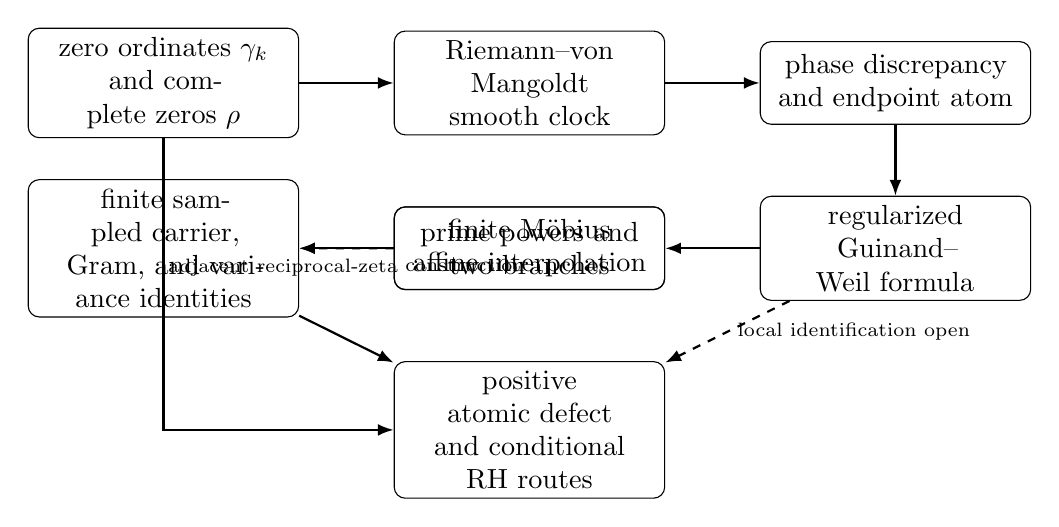
\begin{tikzpicture}[
  node distance=9mm and 12mm,
  box/.style={draw,rounded corners,align=center,text width=3.2cm,minimum height=1.05cm},
  arrow/.style={-{Latex[length=2mm]},thick},
  dashedarrow/.style={-{Latex[length=2mm]},thick,dashed}
]
\node[box] (zeros) {zero ordinates $\gamma_k$\\and complete zeros $\rho$};
\node[box,right=of zeros] (rvm) {Riemann--von Mangoldt\\smooth clock};
\node[box,right=of rvm] (disc) {phase discrepancy\\and endpoint atom};
\node[box,below=of disc] (gw) {regularized\\Guinand--Weil formula};
\node[box,left=of gw] (pp) {prime powers and\\two branches};
\node[box,left=of pp] (finite) {finite sampled carrier,\\Gram, and variance identities};
\node[box,below=of pp] (routes) {positive atomic defect\\and conditional RH routes};
\node[box,below=of rvm] (mobius) {finite Möbius\\affine interpolation};

\draw[arrow] (zeros) -- (rvm);
\draw[arrow] (rvm) -- (disc);
\draw[arrow] (disc) -- (gw);
\draw[arrow] (gw) -- (pp);
\draw[arrow] (pp) -- (finite);
\draw[arrow] (finite) -- (routes);
\draw[arrow] (zeros) |- (routes);
\draw[dashedarrow] (mobius) -- node[below,sloped,font=\scriptsize]
{adjacent reciprocal-zeta construction} (finite);
\draw[dashedarrow] (gw) -- node[right,font=\scriptsize]
{local identification open} (routes);
\end{tikzpicture}
\caption{Logical flow of the manuscript.  Solid arrows indicate proved
constructions or exact reductions.  Dashed arrows indicate an adjacent
construction or an open identification.  In particular, the use of
unweighted prime-power modes as a complete sharp-residual model is not a
proved arrow.}
\label{fig:conceptual_flow}
\end{figure}

\section{Main results and status map}
\label{sec:main_results_status_map}

The following table is a navigation device, not a list of novelty claims.
``Proved here'' means that a complete proof is supplied in this manuscript.

\begin{center}
\begin{tabular}{>{\raggedright\arraybackslash}p{0.31\textwidth}
                >{\raggedright\arraybackslash}p{0.20\textwidth}
                >{\raggedright\arraybackslash}p{0.39\textwidth}}
\toprule
Statement & Status & Precise scope \\
\midrule
Riemann--von Mangoldt counting formula and Guinand--Weil explicit formula
& Classical, unconditional
& Used with the normalization and admissible test class stated in the text. \\
Exact RVM phase-displacement decomposition
& Proved here, unconditional
& Exact for the indexed walk; the quadratic remainder is not proved small. \\
Two prime-power branches
& Classical origin plus exact specialization
& Exact with regularizing weights; completeness of the unweighted sharp model is conjectural. \\
Finite Möbius interpolation
& Proved here, unconditional
& Includes the canonical identity, endpoint value, real-axis limit, rounding, and tail extraction. \\
Positive ordinate-local defect
& Proved here, unconditional
& For one fixed \(q>1\), vanishing of the atomic defect is equivalent to RH. \\
Signed tail \(\Delta_\omega(Q)\)
& Proved here, unconditional
& \(\Delta_\omega(Q)\sim\omega/(\pi^2\log Q)\) in the nonresonant case. \\
Finite carrier and projected variance identities
& Proved here, unconditional
& Exact identities for the chosen finite model and the actual joint projection used numerically. \\
Dominance of the \(n=3\) coefficient system at \(\omega=1\)
& Proved here, unconditional
& Does not by itself imply bimodality of the full radial distribution. \\
Finite spectral alignment from equality on an interval
& Classical linear independence, proved here
& Applies to finite exponential polynomials after grouping repeated frequencies. \\
Seven RH routes
& Conditional implications
& Each implication is rigorous; the activating local or uniform estimate is open. \\
Global asymptotics for the sharp residual
& Conjectural
& No completeness, transport, shell localization, or energy-exhaustion theorem is claimed. \\
Full-data tables and frequency controls
& Numerical
& Finite support only; no asymptotic conclusion is inferred. \\
\bottomrule
\end{tabular}
\end{center}

\section{Notation and logical dependencies}
\label{sec:notation_glossary}

\begin{longtable}{>{\raggedright\arraybackslash}p{0.23\textwidth}
                   >{\raggedright\arraybackslash}p{0.69\textwidth}}
\toprule
Symbol & Meaning \\
\midrule
\endfirsthead
\toprule
Symbol & Meaning \\
\midrule
\endhead
$\gamma_k$ & Positive zero ordinates repeated with multiplicity. \\
$\tau_j,m_j$ & Distinct positive ordinate and its total multiplicity. \\
$N(T),N^{\#}(T)$ & Right-continuous zero count and midpoint count. \\
$\widetilde\gamma_k$ & Inverse RVM clock value satisfying
$N_0(\widetilde\gamma_k)=k-1/2$. \\
$\varepsilon_k$ & Ordinate-clock displacement
$\gamma_k-\widetilde\gamma_k$.  It is not a horizontal displacement and
does not vanish under RH. \\
$\alpha_\rho$ & Horizontal displacement $\beta-1/2$ of a zero
$\rho=\beta+i\gamma$. \\
$q=e^\omega$ & Phase base and angular frequency. \\
$M_H(x)$ & Finite zero kernel
$N(H)^{-1}\sum_{\gamma\leq H}x^{i\gamma}$. \\
$R_N(s)$ & Möbius Dirichlet tail
$\zeta(s)^{-1}-\sum_{n\leq N}\mu(n)n^{-s}$. \\
$\mathcal Q_N(\omega)$ & Quadratic remainder in the indexed phase
linearization; distinct from $R_N(s)$. \\
$\Delta_\omega(Q)$ & Convergent signed prime-power tail. \\
$\widehat c_{Q,H},c_{Q,H}$ & Raw carrier coefficient and jointly fitted
constant--carrier coefficient. \\
\bottomrule
\end{longtable}

\part{The exponential walk and the Riemann--von Mangoldt benchmark}

\section{The zero-counting function and its smooth inverse}
\label{sec:rvm_counting_inverse}

\begin{definition}[Midpoint zero count]
\label{def:midpoint_zero_count}
Let \(N(T)\) be the number of nontrivial zeros \(\rho=\beta+i\gamma\)
with \(0<\gamma\leq T\), counted with multiplicity.  At a zero ordinate
\(T=\tau\), let
\begin{equation}
N^{\#}(\tau)
=
\frac12\left(N(\tau^-)+N(\tau^+)\right).
\label{eq:midpoint_zero_count}
\end{equation}
For a simple ordered ordinate \(\gamma_k\), this equals \(k-1/2\).
\end{definition}

\begin{definition}[Midpoint argument function and exact smooth remainder]
\label{def:rvm_midpoint_argument_remainder}
For \(T\) that is not a zero ordinate, let
\begin{equation}
S(T)
=
\frac1\pi\arg\zeta\!\left(\frac12+iT\right),
\label{eq:rvm_S_function}
\end{equation}
with the standard path from \(2\) to \(2+iT\) and then to
\(1/2+iT\).  At a zero ordinate \(\tau\), define \(S^{\#}(\tau)\) as the
average of the two one-sided limits.  Define
\begin{equation}
R_\vartheta(T)
=
1+\frac{\vartheta(T)}{\pi}-N_0(T),
\label{eq:rvm_exact_smooth_remainder}
\end{equation}
where
\begin{equation}
\vartheta(T)
=
\Im\log\Gamma\!\left(\frac14+\frac{iT}{2}\right)
-
\frac T2\log\pi.
\label{eq:riemann_siegel_theta}
\end{equation}
\end{definition}

\statusnote{Classical result -- unconditional.}
\begin{theorem}[Riemann--von Mangoldt formula]
\label{thm:rvm_formula}
For every \(T>0\), with midpoint interpretation at zero ordinates,
\begin{equation}
\boxed{
N^{\#}(T)
=
N_0(T)+S^{\#}(T)+R_\vartheta(T).
}
\label{eq:rvm_formula}
\end{equation}
Moreover,
\begin{equation}
R_\vartheta(T)=O(T^{-1})
\qquad(T\to\infty).
\label{eq:rvm_remainder}
\end{equation}
The exact counting identity and the asymptotic expansion are standard; see
\cite[Chapter~9]{Titchmarsh1986}.
\end{theorem}

\begin{proof}
For \(T\) that is not a zero ordinate, the argument principle applied to
the completed zeta function
\begin{equation}
\xi(s)
=
\frac12s(s-1)\pi^{-s/2}\Gamma\!\left(\frac s2\right)\zeta(s)
\label{eq:rvm_xi_definition}
\end{equation}
gives the exact identity
\begin{equation}
N(T)
=
1+\frac{\vartheta(T)}{\pi}+S(T).
\label{eq:rvm_theta_exact}
\end{equation}
At a zero ordinate, the average of the two one-sided identities gives the
same formula with \(N^{\#}\) and \(S^{\#}\).  Subtracting \(N_0(T)\) and
using the definition \eqref{eq:rvm_exact_smooth_remainder} proves
\eqref{eq:rvm_formula} exactly.

It remains to estimate \(R_\vartheta\).  Stirling's formula in a fixed
sector gives
\begin{equation}
\log\Gamma(z)
=
\left(z-\frac12\right)\log z-z+\frac12\log(2\pi)
+
O(|z|^{-1}).
\label{eq:rvm_stirling}
\end{equation}
With \(z=1/4+iT/2\), taking imaginary parts yields
\begin{equation}
\vartheta(T)
=
\frac T2\log\!\left(\frac{T}{2\pi}\right)
-
\frac T2
-
\frac\pi8
+
O(T^{-1}).
\label{eq:rvm_theta_asymptotic}
\end{equation}
Consequently,
\begin{align}
1+\frac{\vartheta(T)}{\pi}
&=
\frac{T}{2\pi}\log\!\left(\frac{T}{2\pi e}\right)
+\frac78+O(T^{-1})
\label{eq:rvm_substitution_one}
\\
&=
N_0(T)+O(T^{-1}),
\label{eq:rvm_substitution_two}
\end{align}
which is exactly \eqref{eq:rvm_remainder}.
\end{proof}

\statusnote{Exact result proved in this manuscript -- unconditional.}
\begin{theorem}[Principal Lambert--\(W\) inverse of the smooth clock]
\label{thm:rvm_lambert_inverse}
Let \(x>-1/8\).  The equation \(N_0(T)=x\) has a unique solution
\(T>2\pi\), namely
\begin{equation}
\boxed{
T
=
\frac{2\pi(x-7/8)}
{W_0\!\left((x-7/8)/e\right)}.
}
\label{eq:rvm_lambert_inverse}
\end{equation}
Here \(W_0\) is the principal real branch of the Lambert function
\cite{Corless1996}, and the value at \(x=7/8\) is
understood by continuity as \(T=2\pi e\).  In particular, for every
\(k\geq1\),
\begin{equation}
\widetilde\gamma_k
=
\frac{2\pi(k-11/8)}
{W_0\!\left((k-11/8)/e\right)}.
\label{eq:rvm_gamma_tilde}
\end{equation}
\end{theorem}

\begin{proof}
Put
\begin{equation}
y=x-\frac78,
\qquad
u=\frac{T}{2\pi e}.
\label{eq:rvm_inverse_variables}
\end{equation}
The equation \(N_0(T)=x\) is
\begin{equation}
y=e\,u\log u.
\label{eq:rvm_inverse_step_one}
\end{equation}
Writing \(v=\log u\) gives
\begin{equation}
ve^v=\frac ye.
\label{eq:rvm_inverse_step_two}
\end{equation}
Since \(x>-1/8\), one has \(y/e>-1/e\), so the principal branch
\(W_0(y/e)\) is real and greater than \(-1\).  Thus
\begin{equation}
v=W_0(y/e),
\qquad
u=e^v=\frac{y/e}{W_0(y/e)},
\label{eq:rvm_inverse_step_three}
\end{equation}
and hence \eqref{eq:rvm_lambert_inverse}.  The inequality
\(W_0(y/e)>-1\) implies \(u>e^{-1}\), hence \(T>2\pi\).
Conversely, \(N_0'(T)=(2\pi)^{-1}\log(T/2\pi)>0\) on \((2\pi,\infty)\),
so this solution is unique in that interval.  At \(y=0\),
\(W_0(y/e)\sim y/e\), giving the continuous value \(T=2\pi e\).
Finally, \(x=k-1/2>-1/8\) for every \(k\geq1\), and substitution gives
\eqref{eq:rvm_gamma_tilde}.
\end{proof}

\section{Stieltjes representation and the smooth RVM walk}
\label{sec:stieltjes_rvm_walk}

\begin{definition}[Symmetric phase sum]
\label{def:symmetric_phase_sum}
Define
\begin{equation}
S_\omega^{\#}(T)
=
\sum_{0<\gamma<T}m(\gamma)e^{i\omega\gamma}
+
\frac12
\sum_{\gamma=T}m(\gamma)e^{i\omega\gamma}.
\label{eq:symmetric_phase_sum}
\end{equation}
\end{definition}

\statusnote{Exact result proved in this manuscript -- unconditional.}
\begin{proposition}[Atomic representation and integration by parts]
\label{prop:stieltjes_phase_sum}
Let
\begin{equation}
\dd N
=
\sum_{\gamma>0}m(\gamma)\delta_\gamma.
\label{eq:dN_atomic}
\end{equation}
Then
\begin{equation}
\boxed{
S_\omega^{\#}(T)
=
\int_{(0,T)}e^{i\omega t}\,\dd N(t)
+
\frac12e^{i\omega T}\Delta N(T).
}
\label{eq:stieltjes_phase_sum}
\end{equation}
If \(0<T_0<T\) and neither endpoint is a zero ordinate, then
\begin{align}
\int_{(T_0,T]}e^{i\omega t}\,\dd N(t)
={}&
e^{i\omega T}N(T)-e^{i\omega T_0}N(T_0)
\label{eq:stieltjes_integration_by_parts_one}
\\
&-
i\omega\int_{T_0}^{T}e^{i\omega t}N(t)\,\dd t.
\label{eq:stieltjes_integration_by_parts_two}
\end{align}
The midpoint formula at a zero endpoint is obtained by averaging the two
one-sided identities.
\end{proposition}

\begin{proof}
The first identity is the direct evaluation of the atomic measure
\(\dd N\): atoms strictly below \(T\) receive full weight and the atom at
\(T\) receives half weight.  Merely changing the point value of the
counting function would not change its Stieltjes measure, which is why the
explicit endpoint term is required.

For endpoints away from atoms, \(N\) is a right-continuous
bounded-variation function and \(f(t)=e^{i\omega t}\) is continuously
differentiable.  The Riemann--Stieltjes integration-by-parts formula gives
\begin{equation}
\int_{(T_0,T]} f\,\dd N
=
f(T)N(T)-f(T_0)N(T_0)-\int_{T_0}^{T}N(t)f'(t)\,\dd t.
\label{eq:stieltjes_general_ibp}
\end{equation}
Substitution of \(f'(t)=i\omega e^{i\omega t}\) proves the displayed
formula.  Averaging the limits from the two sides supplies half of any
endpoint atom.
\end{proof}

\begin{warning}[The endpoint term is an atom, not an error term]
\label{warn:endpoint_atom_not_small}
At a zero ordinate $T=\tau$, the boundary contribution in
\eqref{eq:stieltjes_phase_sum} is exactly
\begin{equation}
\frac{m(\tau)}2e^{i\omega\tau}.
\label{eq:endpoint_atom_exact_weight}
\end{equation}
Its modulus is $m(\tau)/2$; it is not naturally small as $T$ grows.  The
right-endpoint convention differs from the midpoint convention by the same
half atom.  Every sharp-window reconstruction in the prime-power part must
retain this term explicitly rather than absorb it into an asymptotic error.
\end{warning}

\statusnote{Exact result proved in this manuscript -- unconditional.}
\begin{theorem}[Smooth Riemann--von Mangoldt contribution]
\label{thm:smooth_rvm_contribution}
The Stieltjes integral of the smooth density
\begin{equation}
N_0'(t)
=
\frac1{2\pi}\log\!\left(\frac{t}{2\pi}\right)
\label{eq:N0_derivative}
\end{equation}
has the antiderivative
\begin{equation}
\boxed{
A_{\mathrm{smooth},\omega}(T)
=
\frac{
 e^{i\omega T}\log(T/2\pi)-\Ei(i\omega T)
}{2\pi i\omega}
+C_\omega.
}
\label{eq:smooth_rvm_antiderivative}
\end{equation}
Consequently, for any \(T_0>0\),
\begin{equation}
\int_{T_0}^{T}e^{i\omega t}N_0'(t)\,\dd t
=
A_{\mathrm{smooth},\omega}(T)
-
A_{\mathrm{smooth},\omega}(T_0).
\label{eq:smooth_rvm_definite}
\end{equation}
\end{theorem}

\begin{proof}
Differentiate the numerator in \eqref{eq:smooth_rvm_antiderivative}.
The derivative of the first term is
\begin{equation}
\frac{\dd}{\dd T}
\left[e^{i\omega T}\log(T/2\pi)\right]
=
i\omega e^{i\omega T}\log(T/2\pi)
+
\frac{e^{i\omega T}}{T}.
\label{eq:smooth_derivative_first}
\end{equation}
Since \(\frac{\dd}{\dd z}\Ei(z)=e^z/z\), the chain rule gives
\begin{equation}
\frac{\dd}{\dd T}\Ei(i\omega T)
=
\frac{e^{i\omega T}}{T}.
\label{eq:smooth_derivative_Ei}
\end{equation}
The two \(T^{-1}\) terms cancel.  Division by \(2\pi i\omega\)
leaves exactly \(e^{i\omega T}N_0'(T)\).  The definite identity follows
from the fundamental theorem of calculus on any interval avoiding the
chosen branch cut; a change of branch alters only the constant
\(C_\omega\).
\end{proof}

\statusnote{Exact result proved in this manuscript -- unconditional.}
\begin{corollary}[Exact RVM remainder decomposition]
\label{cor:rvm_remainder_decomposition}
Let \(0<T_0<T\) and suppose first that neither endpoint is a zero
ordinate.  Then
\begin{align}
\int_{(T_0,T]}e^{i\omega t}\,\dd N(t)
={}&
A_{\mathrm{smooth},\omega}(T)
-
A_{\mathrm{smooth},\omega}(T_0)
\label{eq:rvm_remainder_decomposition_one}
\\
&+
\int_{(T_0,T]}e^{i\omega t}\,\dd S^{\#}(t)
+
\int_{T_0}^{T}e^{i\omega t}R_\vartheta'(t)\,\dd t.
\label{eq:rvm_remainder_decomposition_two}
\end{align}
At a zero endpoint, the corresponding symmetric identity is obtained by
averaging the one-sided limits.
\end{corollary}

\begin{proof}
The exact identity \eqref{eq:rvm_formula} is an equality of locally
bounded-variation functions:
\begin{equation}
N^{\#}(t)=N_0(t)+S^{\#}(t)+R_\vartheta(t).
\label{eq:rvm_linear_decomposition_proof}
\end{equation}
Away from endpoint atoms, taking Stieltjes differentials gives
\begin{equation}
\dd N
=
N_0'(t)\,\dd t+\dd S^{\#}(t)+R_\vartheta'(t)\,\dd t.
\label{eq:rvm_differential_decomposition}
\end{equation}
Integrating against \(e^{i\omega t}\) over \((T_0,T]\) and invoking
Theorem~\ref{thm:smooth_rvm_contribution} for the \(N_0'\)-term proves
the formula.  Midpoint endpoint weights follow from the same one-sided
averaging used in Proposition~\ref{prop:stieltjes_phase_sum}.
\end{proof}

\section{Exact comparison of the indexed zero walk with the smooth clock}
\label{sec:indexed_rvm_comparison}

\begin{definition}
\label{def:index_displacement}
For each \(k\), define the ordinate--clock displacement
\begin{equation}
\varepsilon_k
=
\gamma_k-\widetilde\gamma_k.
\label{eq:index_displacement}
\end{equation}
\end{definition}

\statusnote{Exact result proved in this manuscript -- unconditional.}
\begin{lemma}[Exact phase perturbation identity]
\label{lem:phase_perturbation}
For real \(x\) and \(h\),
\begin{equation}
e^{i(x+h)}-e^{ix}
=
ih\int_0^1e^{i(x+th)}\,\dd t.
\label{eq:phase_perturbation_integral}
\end{equation}
In particular,
\begin{align}
|e^{i(x+h)}-e^{ix}|
&\leq |h|,
\label{eq:phase_lipschitz}
\\
\left|e^{i(x+h)}-e^{ix}-ihe^{ix}\right|
&\leq\frac{h^2}{2}.
\label{eq:phase_quadratic_remainder}
\end{align}
\end{lemma}

\begin{proof}
Define \(F(t)=e^{i(x+th)}\) on \([0,1]\).  Since
\(F'(t)=ihe^{i(x+th)}\), the fundamental theorem of calculus gives
\begin{equation}
e^{i(x+h)}-e^{ix}
=
F(1)-F(0)
=
ih\int_0^1e^{i(x+th)}\,\dd t.
\label{eq:phase_perturbation_ftc_detailed}
\end{equation}
The integrand has modulus one, so taking absolute values yields the
Lipschitz estimate.  For the quadratic estimate, subtract \(ihe^{ix}\):
\begin{equation}
e^{i(x+h)}-e^{ix}-ihe^{ix}
=
ihe^{ix}\int_0^1(e^{ith}-1)\,\dd t.
\label{eq:phase_quadratic_identity_detailed}
\end{equation}
Apply the already proved Lipschitz bound to \(e^{ith}-1\), obtaining
\(|e^{ith}-1|\leq t|h|\).  Integration of \(t\) from zero to one gives
\(h^2/2\).
\end{proof}

\statusnote{Exact result proved in this manuscript -- unconditional.}
\begin{theorem}[Exact and first-order decompositions of the discrepancy]
\label{thm:indexed_discrepancy_decomposition}
For every \(N\),
\begin{equation}
\mathcal E_N(\omega)
=
i\omega
\sum_{k=1}^{N}
\varepsilon_k
\int_0^1
 e^{i\omega(\widetilde\gamma_k+t\varepsilon_k)}\,\dd t.
\label{eq:exact_indexed_discrepancy}
\end{equation}
Moreover,
\begin{equation}
\mathcal E_N(\omega)
=
i\omega\sum_{k=1}^{N}
\varepsilon_ke^{i\omega\widetilde\gamma_k}
+
\mathcal Q_N(\omega),
\label{eq:first_order_indexed_discrepancy}
\end{equation}
where
\begin{equation}
|\mathcal Q_N(\omega)|
\leq
\frac{\omega^2}{2}
\sum_{k=1}^{N}\varepsilon_k^2.
\label{eq:indexed_discrepancy_remainder}
\end{equation}
\end{theorem}

\begin{proof}
For each \(k\), apply Lemma~\ref{lem:phase_perturbation} to
\begin{equation}
x=\omega\widetilde\gamma_k,
\qquad
h=\omega(\gamma_k-\widetilde\gamma_k)=\omega\varepsilon_k.
\label{eq:indexed_discrepancy_substitution}
\end{equation}
The resulting identity is
\begin{equation}
e^{i\omega\gamma_k}-e^{i\omega\widetilde\gamma_k}
=
i\omega\varepsilon_k
\int_0^1e^{i\omega(\widetilde\gamma_k+t\varepsilon_k)}\,\dd t.
\label{eq:indexed_discrepancy_termwise}
\end{equation}
Summing from \(1\) to \(N\) gives the exact formula.  For the first-order
form, the quadratic estimate in the lemma gives a remainder \(r_k\) with
\begin{equation}
|r_k|\leq\frac{\omega^2\varepsilon_k^2}{2}.
\label{eq:indexed_term_remainder_bound}
\end{equation}
The triangle inequality then gives the stated bound for the sum of all
remainders.  No restriction on the signs or dependence of the ordinate--clock displacements
is needed.
\end{proof}

\begin{definition}[Midpoint rank of a distinct ordinate]
\label{def:midpoint_rank_distinct_ordinate}
Let
\begin{equation}
0<\tau_1<\tau_2<\cdots.
\label{eq:distinct_ordinate_order}
\end{equation}
be the distinct positive zero ordinates, and let \(m_j\) be the total
multiplicity at \(\tau_j\).  Define the midpoint rank
\begin{equation}
\kappa_j
=
N(\tau_j^-)+\frac{m_j}{2}
=
N^{\#}(\tau_j),
\label{eq:midpoint_rank_distinct_ordinate}
\end{equation}
the smooth comparison ordinate
\begin{equation}
\widetilde\tau_j
=
N_0^{-1}(\kappa_j),
\label{eq:smooth_distinct_ordinate}
\end{equation}
and the displacement
\begin{equation}
\varepsilon_j^{\#}
=
\tau_j-\widetilde\tau_j.
\label{eq:distinct_ordinate_displacement}
\end{equation}
\end{definition}

\statusnote{Exact result proved in this manuscript -- unconditional.}
\begin{proposition}[Displacement in terms of the Riemann--von Mangoldt remainder]
\label{prop:displacement_rvm_remainder}
For every distinct positive zero ordinate \(\tau_j\), there is a point
\(\xi_j\) between \(\tau_j\) and \(\widetilde\tau_j\) such that
\begin{equation}
\boxed{
\varepsilon_j^{\#}
=
-
\frac{S^{\#}(\tau_j)+R_\vartheta(\tau_j)}
{N_0'(\xi_j)}.
}
\label{eq:displacement_rvm_formula}
\end{equation}
Equivalently,
\begin{equation}
\varepsilon_j^{\#}
=
-
\frac{2\pi\,[S^{\#}(\tau_j)+R_\vartheta(\tau_j)]}
{\log(\xi_j/2\pi)}.
\label{eq:displacement_rvm_explicit}
\end{equation}
If \(\tau_j\) is simple and is the \(j\)-th ordinate when ordinates are
listed with multiplicity, then
\(\kappa_j=j-\tfrac12\),
\(\widetilde\tau_j=\widetilde\gamma_j\), and
\(\varepsilon_j^{\#}=\varepsilon_j\).
\end{proposition}

\begin{proof}
By Definitions~\ref{def:midpoint_zero_count} and
\ref{def:midpoint_rank_distinct_ordinate},
\begin{equation}
N_0(\widetilde\tau_j)
=
\kappa_j
=
N^{\#}(\tau_j).
\label{eq:displacement_count_equalities}
\end{equation}
The exact Riemann--von Mangoldt identity
\eqref{eq:rvm_formula} therefore gives
\begin{equation}
N_0(\widetilde\tau_j)-N_0(\tau_j)
=
S^{\#}(\tau_j)+R_\vartheta(\tau_j).
\label{eq:displacement_count_difference}
\end{equation}
Both \(\tau_j\) and \(\widetilde\tau_j\) exceed \(2\pi\), so \(N_0\) is
differentiable on the closed interval joining them and
\(N_0'(t)=(2\pi)^{-1}\log(t/2\pi)>0\) there.  The mean-value theorem
provides \(\xi_j\) between the two ordinates such that
\begin{align}
N_0(\widetilde\tau_j)-N_0(\tau_j)
&=
N_0'(\xi_j)(\widetilde\tau_j-\tau_j)
\label{eq:displacement_mvt_first}
\\
&=
-N_0'(\xi_j)\varepsilon_j^{\#}.
\label{eq:displacement_mvt}
\end{align}
Solving for \(\varepsilon_j^{\#}\) gives
\eqref{eq:displacement_rvm_formula}; substitution of the explicit
derivative gives \eqref{eq:displacement_rvm_explicit}.  In the simple
case \(m_j=1\) and \(N(\tau_j^-)=j-1\), so
\(\kappa_j=j-\tfrac12\), proving the final assertion.
\end{proof}


\subsection{Magnitude of the quadratic displacement sum}
\label{subsec:rvm_displacement_square_size}

The indexed phase remainder in \eqref{eq:indexed_discrepancy_remainder}
contains the displacements \(\varepsilon_k\) attached to the list repeated
with multiplicity.  The exact Riemann--von Mangoldt formula at a multiple
ordinate naturally gives instead the midpoint displacement
\(\varepsilon_j^{\#}\).  The following identity keeps those two objects
separate.

\statusnote{Exact result proved in this manuscript -- unconditional.}
\begin{proposition}[Multiplicity correction between indexed and atomic clocks]
\label{prop:multiplicity_clock_correction}
Let \(\tau_j\) have multiplicity \(m_j\), let
\(a_j=N(\tau_j^-)\), and write the corresponding repeated indices as
\(k=a_j+r\), \(1\leq r\leq m_j\).  Put
\begin{equation}
\theta_{j,r}=r-\frac{m_j+1}{2}.
\label{eq:multiplicity_centered_rank}
\end{equation}
There exists a point \(\xi_{j,r}\) between
\(\widetilde\tau_j\) and \(\widetilde\gamma_{a_j+r}\) such that
\begin{equation}
\boxed{
\varepsilon_{a_j+r}
=
\varepsilon_j^{\#}
-
\frac{\theta_{j,r}}{N_0'(\xi_{j,r})}.
}
\label{eq:indexed_atomic_displacement_relation}
\end{equation}
Consequently,
\begin{equation}
\sum_{r=1}^{m_j}|\varepsilon_{a_j+r}|^2
\leq
2m_j|\varepsilon_j^{\#}|^2
+
\frac{m_j(m_j^2-1)}{6\,d_j^2},
\label{eq:multiplicity_square_correction}
\end{equation}
where
\begin{equation}
d_j=
\min_{t\text{ between }\widetilde\tau_j
\text{ and all }\widetilde\gamma_{a_j+r}}N_0'(t)>0.
\label{eq:multiplicity_min_derivative}
\end{equation}
For a simple zero, \(m_j=1\) and the correction term vanishes.
\end{proposition}

\begin{proof}
The midpoint rank is
\(\kappa_j=a_j+m_j/2\), whereas the repeated index \(a_j+r\)
uses rank \(a_j+r-1/2\).  Their difference is exactly
\begin{equation}
(a_j+r-1/2)-\kappa_j=\theta_{j,r}.
\label{eq:rank_difference_exact}
\end{equation}
Apply the mean-value theorem to the inverse relation
\(N_0(\widetilde\gamma_k)=k-1/2\):
\begin{equation}
\widetilde\gamma_{a_j+r}-\widetilde\tau_j
=
\frac{\theta_{j,r}}{N_0'(\xi_{j,r})}.
\label{eq:smooth_clock_rank_mvt}
\end{equation}
Subtract this identity from
\(\tau_j-\widetilde\tau_j=\varepsilon_j^{\#}\) to obtain
\eqref{eq:indexed_atomic_displacement_relation}.  The inequality
\(|x-y|^2\leq2|x|^2+2|y|^2\), followed by
\begin{equation}
\sum_{r=1}^{m_j}\theta_{j,r}^2
=
\frac{m_j(m_j^2-1)}{12},
\label{eq:centered_rank_square_sum}
\end{equation}
proves \eqref{eq:multiplicity_square_correction}.
\end{proof}

\begin{definition}
\label{def:rvm_square_sums}
Define the atomic-midpoint and repeated-index square sums by
\begin{align}
\mathscr E_2^{\#}(T)
&=
\sum_{0<\tau_j\leq T}m_j|\varepsilon_j^{\#}|^2,
\label{eq:rvm_E2_atomic_global}
\\
\mathscr E_2^{\mathrm{idx}}(T)
&=
\sum_{\gamma_k\leq T}|\varepsilon_k|^2,
\label{eq:rvm_E2_index_global}
\end{align}
and define their windowed analogues by restricting the ordinates to
\((T,T+L]\).
\end{definition}

\statusnote{Bounds deduced from classical estimates -- unconditional unless RH is explicitly assumed.}
\begin{proposition}[Crude global and short-window bounds]
\label{prop:rvm_displacement_square_bounds}
For \(1\leq L\leq T\),
\begin{align}
\mathscr E_2^{\#}(T),\ \mathscr E_2^{\mathrm{idx}}(T)
&=O(T\log T),
\label{eq:rvm_E2_unconditional_global}
\\
\mathscr E_2^{\#}(T;L),\ \mathscr E_2^{\mathrm{idx}}(T;L)
&=O(L\log T+\log T).
\label{eq:rvm_E2_unconditional_window}
\end{align}
Under RH,
\begin{align}
\mathscr E_2^{\#}(T),\ \mathscr E_2^{\mathrm{idx}}(T)
&=
O\!\left(\frac{T\log T}{(\log\log T)^2}\right),
\label{eq:rvm_E2_RH_global}
\\
\mathscr E_2^{\#}(T;L),\ \mathscr E_2^{\mathrm{idx}}(T;L)
&=
O\!\left(
\frac{L\log T+\log T}{(\log\log T)^2}
\right).
\label{eq:rvm_E2_RH_window}
\end{align}
The implied constants may depend on a fixed lower height.  None of these
bounds makes the unnormalized quadratic phase remainder small.
\end{proposition}

\begin{corollary}[What the available square-sum bounds actually imply]
\label{cor:rvm_square_sum_interpretation}
With \(N(T)\sim (T/2\pi)\log T\), the global bounds imply
\begin{align}
\frac{\mathscr E_2^{\#}(T)}{N(T)},\;
\frac{\mathscr E_2^{\mathrm{idx}}(T)}{N(T)}
&=O(1),
\label{eq:rvm_global_mean_square_unconditional}
\\
\frac{\mathscr E_2^{\#}(T)}{N(T)},\;
\frac{\mathscr E_2^{\mathrm{idx}}(T)}{N(T)}
&=O\!\left(\frac1{(\log\log T)^2}\right)
\quad\text{under RH}.
\label{eq:rvm_global_mean_square_RH}
\end{align}
For a fixed-length window, the unconditional estimate remains only
\begin{equation}
\mathscr E_2^{\#}(T;L),\;
\mathscr E_2^{\mathrm{idx}}(T;L)=O(\log T)
\qquad(L\asymp1),
\label{eq:rvm_fixed_window_square_sum}
\end{equation}
and does not tend to zero.  Hence the displacement is globally bounded in
mean square, and under RH globally small on average, but no presently used
bound supplies uniform local smallness on every short window.
\end{corollary}

\begin{remark}[Why the quadratic phase remainder remains decisive]
\label{rem:rvm_quadratic_remainder_decisive}
The exact estimate
\begin{equation}
|\mathcal Q_N(\omega)|
\leq
\frac{\omega^2}{2}
\sum_{k\leq N}|\varepsilon_k|^2
\label{eq:rvm_quadratic_remainder_recalled}
\end{equation}
therefore cannot be turned into \(o(1)\), or even into an error smaller
than the first-order term, from the preceding bounds alone.  Three distinct
questions remain: global average control, control after localization by a
smooth compactly supported weight, and uniform control in windows of length
comparable with \(1/\omega\).  The last two are the ones required by the
local routes to RH.
\end{remark}

\begin{proof}
Proposition~\ref{prop:displacement_rvm_remainder} and
\(N_0'(t)=(2\pi)^{-1}\log(t/2\pi)\) give, for large ordinates,
\begin{equation}
|\varepsilon_j^{\#}|
\ll
\frac{|S^{\#}(\tau_j)|+O(\tau_j^{-1})}{\log\tau_j}.
\label{eq:rvm_epsilon_bound_from_S}
\end{equation}
The classical unconditional estimate \(S(T)=O(\log T)\) therefore gives
\(|\varepsilon_j^{\#}|=O(1)\).  Under RH, Littlewood's bound gives
\(|\varepsilon_j^{\#}|=O(1/\log\log T)\).  The local zero count
\begin{equation}
N(T+L)-N(T)=O(L\log T+\log T)
\label{eq:rvm_local_zero_count}
\end{equation}
then proves the asserted atomic-midpoint bounds.

For the repeated-index sum, use
Proposition~\ref{prop:multiplicity_clock_correction}.  The multiplicity at
height \(t\) obeys
\begin{equation}
m(t)\leq N(t+1)-N(t-1)=O(\log t),
\label{eq:multiplicity_crude_bound}
\end{equation}
Under RH, the jump relation for \(S\), together with Littlewood's bound,
gives
\begin{equation}
m(t)=O\!\left(\frac{\log t}{\log\log t}\right).
\label{eq:multiplicity_RH_bound}
\end{equation}
Since every relevant derivative
\(d_j\asymp\log T\) on a fixed high window, one has
\begin{equation}
\sum_j\frac{m_j(m_j^2-1)}{d_j^2}
\ll
\frac{(\max_j m_j)^2}{(\log T)^2}\sum_jm_j.
\label{eq:multiplicity_correction_summed}
\end{equation}
Unconditionally \(\max_jm_j=O(\log T)\), while under RH
\(\max_jm_j=O(\log T/\log\log T)\).  Since \(\sum_jm_j\) is the
ordinary zero count in the relevant global interval or short window,
\eqref{eq:multiplicity_correction_summed} has precisely the orders asserted
above.  This proves the indexed bounds.  The
bounds for \(S\), multiplicities, and zero counts are standard; see
\cite[Chapters~9 and~14]{Titchmarsh1986}.
\end{proof}

\begin{warning}[What these bounds do not establish]
\label{warn:rvm_square_sum_not_RH}
The ordinate-clock displacements \(\varepsilon_k\) and
\(\varepsilon_j^{\#}\) are not horizontal displacements
\(\beta-1/2\).  RH does not force them to vanish; even on RH the ordinates
fluctuate around the RVM clock through \(S(T)\).  Consequently, a bound for
these square sums is not an equivalent form of RH.  Continuous mean-square
information for \(S(t)\) also does not automatically control its values at
zero ordinates in windows of fixed length.  A route based on
\eqref{eq:indexed_discrepancy_remainder} needs a genuinely discrete and
local estimate.
\end{warning}

\begin{remark}
\label{rem:rvm_origin_prime_formula}
Equations \eqref{eq:first_order_indexed_discrepancy} and
\eqref{eq:displacement_rvm_explicit} explain why a comparison with the RVM
clock is sensitive to the argument of zeta.  The explicit formula then
rewrites that argument contribution in terms of prime powers.  This is the
analytic route by which the prime-power branches entered the project.
\end{remark}

\part{Finite Möbius interpolation}


\section{The first affine interpolation: numerical and symbolic forms}
\label{sec:first_affine_interpolation}

\begin{definition}[Terminal affine interpolation]
\label{def:terminal_affine_interpolation}
Let \(Q_N=\{q_1,\ldots,q_{h_N}\}\) be the primes in \((N/2,N]\), and
let \(A_N,P_N,B_N\) be defined in Section~\ref{sec:mobius_definitions}.
For a prescribed terminal sum \(m\in\mathbb C\), define
\begin{equation}
\boxed{
\mathcal I_N(s;m)
=
A_N(s)+\frac{m-B_N}{h_N}P_N(s).
}
\label{eq:terminal_affine_interpolation}
\end{equation}
This is the symmetric affine interpolation in which all terminal-prime
coefficients are assigned their common mean
\begin{equation}
\lambda_N(m)=\frac{m-B_N}{h_N}.
\label{eq:terminal_mean_coefficient}
\end{equation}
\end{definition}

\statusnote{Exact result proved in this manuscript -- unconditional.}
\begin{proposition}[Recovery of the true finite Möbius polynomial]
\label{prop:true_terminal_value}
For the true Mertens value \(m=M(N)\),
\begin{equation}
\mathcal I_N(s;M(N))
=
M_s(N).
\label{eq:true_terminal_interpolation}
\end{equation}
\end{proposition}

\begin{proof}
The set \(Q_N\) contains only primes, so every terminal Möbius coefficient
is exactly \(-1\).  Therefore its total contribution at \(s=0\) is
\(-h_N\), which proves \(M(N)=B_N-h_N\).  Hence the affine mean coefficient
for the true terminal value is
\begin{equation}
\frac{M(N)-B_N}{h_N}
=
\frac{-h_N}{h_N}
=-1.
\label{eq:true_terminal_mean_proof_detailed}
\end{equation}
Substitution assigns coefficient \(-1\) to every term in \(P_N(s)\), so
\begin{equation}
\mathcal I_N(s;M(N))
=
A_N(s)-P_N(s).
\label{eq:true_terminal_interpolation_proof_detailed}
\end{equation}
The right side is exactly the decomposition of \(M_s(N)\).
\end{proof}

\begin{example}[The numerical model \(N=10\)]
\label{ex:N10_affine_interpolation}
The Möbius values up to ten are
\begin{equation}
(1,-1,-1,0,-1,1,-1,0,0,1).
\label{eq:N10_mobius_vector}
\end{equation}
The only terminal prime is \(7\), so
\begin{align}
Q_{10}&=\{7\},
&h_{10}&=1,
&P_{10}(s)&=7^{-s},
\label{eq:N10_terminal_data_detailed}
\\
A_{10}(s)
&=
1-2^{-s}-3^{-s}-5^{-s}+6^{-s}+10^{-s},
&B_{10}&=0.
\label{eq:N10_A_B_detailed}
\end{align}
Thus
\begin{equation}
\mathcal I_{10}(s;m)
=
A_{10}(s)+m7^{-s}.
\label{eq:N10_interpolation_detailed}
\end{equation}
The actual terminal value is \(M(10)=-1\), which restores the coefficient
\(-1\) of \(7^{-s}\).
\end{example}

\statusnote{Exact result proved in this manuscript -- unconditional.}
\begin{theorem}[Completion equation]
\label{thm:completion_equation}
At every point where \(P_N(s)\neq0\), the unique value of \(m\) satisfying
\begin{equation}
\mathcal I_N(s;m)=\zeta(s)^{-1}
\label{eq:completion_equation}
\end{equation}
is
\begin{equation}
\boxed{
 m=\Phi_N(s)
 =
 B_N+h_N\frac{\zeta(s)^{-1}-A_N(s)}{P_N(s)}.
}
\label{eq:completion_solution}
\end{equation}
\end{theorem}

\begin{proof}
Starting from the affine interpolation, the completion equation is
\begin{equation}
A_N(s)+\frac{m-B_N}{h_N}P_N(s)
=
\zeta(s)^{-1}.
\label{eq:completion_equation_expanded}
\end{equation}
Because \(h_N\neq0\) and \(P_N(s)\neq0\), this is a nondegenerate linear
equation in \(m\).  Subtract \(A_N(s)\), multiply by \(h_N/P_N(s)\), and
add \(B_N\) to obtain the displayed solution.  If two values \(m_1,m_2\)
solved the equation, subtracting their equations would give
\begin{equation}
\frac{m_1-m_2}{h_N}P_N(s)=0,
\label{eq:completion_uniqueness}
\end{equation}
so \(m_1=m_2\).  This proves both existence and uniqueness.
\end{proof}

\begin{remark}
\label{rem:Phi_meaning}
The function \(\Phi_N(s)\) is therefore not introduced by an arbitrary
quotient.  It is the terminal value selected by requiring the affine finite
interpolation to coincide with the completed reciprocal-zeta Dirichlet
series at the spectral parameter \(s\).
\end{remark}

\section{Terminal half-interval decomposition}
\label{sec:mobius_definitions}

\begin{definition}
\label{def:terminal_prime_set}
For an integer \(N\geq 2\), define
\begin{equation}
Q_N
=
\left\{
q\ \text{prime}:\frac{N}{2}<q\leq N
\right\},
\label{eq:terminal_prime_set}
\end{equation}
and put
\begin{equation}
h_N=|Q_N|,
\qquad
q_N=\min Q_N.
\label{eq:hN_qN}
\end{equation}
Bertrand's postulate guarantees \(h_N\geq 1\).
\end{definition}

\begin{definition}
\label{def:mobius_polynomials}
Let
\begin{align}
M_s(N)
&=
\sum_{n\leq N}\frac{\mu(n)}{n^s},
\label{eq:MsN_definition}
\\
P_N(s)
&=
\sum_{q\in Q_N}q^{-s},
\label{eq:PN_definition}
\\
A_N(s)
&=
\sum_{\substack{n\leq N\\n\notin Q_N}}
\frac{\mu(n)}{n^s},
\label{eq:AN_definition}
\\
B_N
&=
A_N(0)
=
\sum_{\substack{n\leq N\\n\notin Q_N}}\mu(n).
\label{eq:BN_definition}
\end{align}
Since every \(q\in Q_N\) is prime and \(\mu(q)=-1\),
\begin{equation}
M_s(N)=A_N(s)-P_N(s)
\label{eq:Ms_A_minus_P}
\end{equation}
and
\begin{equation}
M(N)=B_N-h_N.
\label{eq:M_B_minus_h}
\end{equation}
\end{definition}

\begin{definition}
\label{def:tail_RN}
For \(\Re s>1\), define the exact tail
\begin{equation}
R_N(s)
=
\frac{1}{\zeta(s)}-M_s(N)
=
\sum_{n>N}\frac{\mu(n)}{n^s}.
\label{eq:RN_definition}
\end{equation}
The first equality supplies a meromorphic continuation of \(R_N\).
\end{definition}

\begin{definition}
\label{def:PhiN}
Define
\begin{equation}
\Phi_N(s)
=
B_N+
h_N\frac{\zeta(s)^{-1}-A_N(s)}{P_N(s)}
\label{eq:PhiN_definition}
\end{equation}
at points at which the quotient is defined, and meromorphically elsewhere.
\end{definition}

\section{Canonical identity and endpoint values}
\label{sec:canonical_identity}

\statusnote{Exact result proved in this manuscript -- unconditional.}
\begin{theorem}[Canonical orientation]
\label{thm:canonical_orientation}
For every \(N\geq2\),
\begin{equation}
\boxed{
\Phi_N(s)
=
B_N+
h_N\frac{\zeta(s)^{-1}-A_N(s)}{P_N(s)}
=
M(N)+h_N\frac{R_N(s)}{P_N(s)}.
}
\label{eq:canonical_orientation}
\end{equation}
\end{theorem}

\begin{proof}
The functions \(A_N(s)\) and \(P_N(s)\) are finite Dirichlet polynomials
and hence entire.  In the half-plane \(\Re s>1\), absolute convergence of
the reciprocal-zeta Dirichlet series gives
\begin{equation}
\zeta(s)^{-1}
=
M_s(N)+R_N(s).
\label{eq:canonical_proof_reciprocal_split}
\end{equation}
The terminal decomposition \(M_s(N)=A_N(s)-P_N(s)\) therefore yields
\begin{align}
\zeta(s)^{-1}-A_N(s)
&=
M_s(N)+R_N(s)-A_N(s)
\label{eq:canonical_proof_step_one}
\\
&=
R_N(s)-P_N(s).
\label{eq:canonical_proof_step_two}
\end{align}
Divide by \(P_N(s)\) at a point where it is nonzero, multiply by \(h_N\),
and add \(B_N\):
\begin{align}
\Phi_N(s)
&=
B_N+h_N\left(\frac{R_N(s)}{P_N(s)}-1\right)
\label{eq:canonical_proof_step_three}
\\
&=
B_N-h_N+h_N\frac{R_N(s)}{P_N(s)}.
\label{eq:canonical_proof_step_four}
\end{align}
Because the terminal primes all have Möbius value \(-1\),
\(M(N)=B_N-h_N\).  This proves the identity on \(\Re s>1\).  Both sides
are meromorphic continuations of the same function, so the identity extends
to every connected component of their common domain and hence
meromorphically to the plane.
\end{proof}

\statusnote{Exact result proved in this manuscript -- unconditional.}
\begin{corollary}[Value at the origin]
\label{cor:Phi_origin}
The meromorphic interpolation satisfies
\begin{equation}
\boxed{\Phi_N(0)=-2.}
\label{eq:Phi_origin}
\end{equation}
\end{corollary}

\begin{proof}
The point \(s=0\) is regular for every finite Dirichlet polynomial in the
formula.  The classical special value \(\zeta(0)=-1/2\) gives
\begin{equation}
\zeta(0)^{-1}=-2.
\label{eq:origin_inverse_zeta}
\end{equation}
Moreover, by definition,
\begin{equation}
A_N(0)=B_N,
\qquad
P_N(0)=\sum_{q\in Q_N}1=h_N.
\label{eq:origin_finite_values}
\end{equation}
Since \(h_N\geq1\), the denominator does not vanish.  Direct substitution
in the completion solution gives
\begin{align}
\Phi_N(0)
&=
B_N+h_N\frac{-2-B_N}{h_N}
\label{eq:origin_substitution_detailed}
\\
&=
B_N-2-B_N
=-2.
\label{eq:origin_cancellation_detailed}
\end{align}
No limiting argument is involved.
\end{proof}

\statusnote{Exact result proved in this manuscript -- unconditional.}
\begin{corollary}[Large positive real limit]
\label{cor:Phi_infinity}
Along the positive real axis,
\begin{equation}
\boxed{
\lim_{\sigma\to+\infty}\Phi_N(\sigma)=M(N).
}
\label{eq:Phi_infinity}
\end{equation}
\end{corollary}

\begin{proof}
For \(\sigma>1\), the tail satisfies
\begin{equation}
|R_N(\sigma)|
\leq
\sum_{n>N}n^{-\sigma}
\leq
\int_N^\infty x^{-\sigma}\,\dd x
=
\frac{N^{1-\sigma}}{\sigma-1}.
\label{eq:infinity_tail_bound}
\end{equation}
The term \(q_N^{-\sigma}\) occurs in \(P_N(\sigma)\), and all terms are
positive, hence
\begin{equation}
P_N(\sigma)\geq q_N^{-\sigma}.
\label{eq:infinity_denominator_bound}
\end{equation}
Consequently,
\begin{equation}
\left|h_N\frac{R_N(\sigma)}{P_N(\sigma)}\right|
\leq
\frac{h_NN}{\sigma-1}
\left(\frac{q_N}{N}\right)^\sigma.
\label{eq:infinity_ratio_bound}
\end{equation}
For \(N\geq3\), Bertrand's theorem gives a prime in \((N/2,N)\), so
\(q_N<N\), and the exponential factor tends to zero.  For \(N=2\),
\(q_N/N=1\), but the same bound is \(2/(\sigma-1)\), which also tends to
zero.  Hence the second expression in
Theorem~\ref{thm:canonical_orientation} tends to \(M(N)\) for every
\(N\geq2\).
\end{proof}

\begin{example}[The \(N=10\) orientation check]
\label{exp:N10_orientation}
For \(N=10\),
\begin{equation}
Q_{10}=\{7\},
\qquad
h_{10}=1,
\qquad
M(10)=-1,
\qquad
B_{10}=0.
\label{eq:N10_data}
\end{equation}
The inverted quotient \(P_N/R_N\) would give \(-1/2\) at \(s=0\).
The quotient in \eqref{eq:canonical_orientation} gives
\begin{equation}
0+\frac{-2}{1}=-2.
\label{eq:N10_correct_value}
\end{equation}
This finite check confirms the orientation of the quotient in Theorem~\ref{thm:canonical_orientation}.
\end{example}

\section{Exponential approach, rounding, and recovery of the first tail term}
\label{sec:asymptotic_recovery}

\begin{definition}
\label{def:aN}
Let
\begin{equation}
a_N
=
\min\{n>N:\mu(n)\neq0\}.
\label{eq:aN_definition}
\end{equation}
\end{definition}

\statusnote{Exact result proved in this manuscript -- unconditional.}
\begin{theorem}[Leading exponential term]
\label{thm:leading_exponential}
As \(\sigma\to+\infty\),
\begin{equation}
\boxed{
\Phi_N(\sigma)-M(N)
=
h_N\mu(a_N)
\left(\frac{q_N}{a_N}\right)^\sigma
\left(1+o(1)\right).
}
\label{eq:leading_exponential}
\end{equation}
\end{theorem}

\begin{proof}
Factor the least terminal prime from the denominator:
\begin{equation}
P_N(\sigma)
=
q_N^{-\sigma}
\left[
1+
\sum_{\substack{q\in Q_N\\q>q_N}}
\left(\frac{q_N}{q}\right)^\sigma
\right].
\label{eq:leading_P_factorization}
\end{equation}
Every ratio in the bracket is strictly smaller than one, and there are only
finitely many of them.  Thus the bracket is \(1+o(1)\).

For the numerator, factor the first nonzero Möbius term after \(N\):
\begin{equation}
R_N(\sigma)
=
\mu(a_N)a_N^{-\sigma}
\left[
1+
\sum_{n>a_N}
\frac{\mu(n)}{\mu(a_N)}
\left(\frac{a_N}{n}\right)^\sigma
\right].
\label{eq:leading_R_factorization}
\end{equation}
For \(\sigma\geq2\), the absolute value of the summand is bounded by
\((a_N/n)^2\), whose sum over \(n>a_N\) is finite.  Each fixed summand
tends to zero as \(\sigma\to\infty\).  Dominated convergence therefore
shows that the bracket is \(1+o(1)\).  Division gives
\begin{equation}
\frac{R_N(\sigma)}{P_N(\sigma)}
=
\mu(a_N)
\left(\frac{q_N}{a_N}\right)^\sigma
(1+o(1)).
\label{eq:leading_ratio_detailed}
\end{equation}
Multiply by \(h_N\) and use the canonical identity.
\end{proof}

\begin{remark}[Existence of the root limit and absence of leading cancellation]
\label{rem:aN_no_cancellation}
The limit in Corollary~\ref{cor:aN_recovery} is not an additional
hypothesis.  The integer $a_N$ is the unique least index with nonzero tail
coefficient.  After factoring $\mu(a_N)a_N^{-\sigma}$, the remaining
absolute tail is dominated by $\sum_{n>a_N}(a_N/n)^2$ and tends to zero by
dominated convergence.  Hence the leading term cannot be cancelled by later
terms for all sufficiently large real $\sigma$.
\end{remark}

\begin{remark}
\label{rem:orientation_growth}
The factor is \((q_N/a_N)^\sigma\), not
\((a_N/q_N)^\sigma\).  Since \(q_N\leq N<a_N\), the correct factor
decays.  The inverted factor would contradict
Corollary~\ref{cor:Phi_infinity}.
\end{remark}

\statusnote{Exact result proved in this manuscript -- unconditional.}
\begin{theorem}[Uniform real-axis error bound]
\label{thm:rounding_bound}
For every real \(\sigma>1\),
\begin{equation}
\boxed{
|\Phi_N(\sigma)-M(N)|
\leq
\frac{h_NN}{\sigma-1}
\left(\frac{q_N}{N}\right)^\sigma.
}
\label{eq:rounding_bound}
\end{equation}
\end{theorem}

\begin{proof}
The reciprocal-zeta tail is absolutely convergent for \(\sigma>1\), so
\begin{align}
|R_N(\sigma)|
&\leq
\sum_{n>N}|\mu(n)|n^{-\sigma}
\label{eq:rounding_abs_mu}
\\
&\leq
\sum_{n>N}n^{-\sigma}
\label{eq:rounding_drop_mu}
\\
&\leq
\int_N^\infty x^{-\sigma}\,\dd x
=
\frac{N^{1-\sigma}}{\sigma-1}.
\label{eq:rounding_integral_detailed}
\end{align}
The denominator is a sum of positive real terms.  Retaining only its
largest term gives
\begin{equation}
P_N(\sigma)
=
\sum_{q\in Q_N}q^{-\sigma}
\geq
q_N^{-\sigma}.
\label{eq:rounding_P_positive}
\end{equation}
The canonical identity now gives
\begin{align}
|\Phi_N(\sigma)-M(N)|
&=
h_N\frac{|R_N(\sigma)|}{P_N(\sigma)}
\label{eq:rounding_identity_use}
\\
&\leq
\frac{h_NN^{1-\sigma}q_N^\sigma}{\sigma-1}
\label{eq:rounding_combine}
\\
&=
\frac{h_NN}{\sigma-1}
\left(\frac{q_N}{N}\right)^\sigma.
\label{eq:rounding_final_detailed}
\end{align}
\end{proof}

\statusnote{Exact result proved in this manuscript -- unconditional.}
\begin{corollary}[Finite rounding criterion]
\label{cor:rounding_criterion}
If
\begin{equation}
\boxed{
\frac{h_NN}{\sigma-1}
\left(\frac{q_N}{N}\right)^\sigma
<
\frac12,
}
\label{eq:rounding_criterion}
\end{equation}
then \(M(N)\) is the unique nearest integer to the real number
\(\Phi_N(\sigma)\).
\end{corollary}

\begin{proof}
Theorem~\ref{thm:rounding_bound} and
\eqref{eq:rounding_criterion} give
\begin{equation}
|\Phi_N(\sigma)-M(N)|<\frac12.
\label{eq:rounding_criterion_proof_ball}
\end{equation}
For any integer \(k\neq M(N)\), the reverse triangle inequality yields
\begin{align}
|\Phi_N(\sigma)-k|
&\geq
|k-M(N)|-|\Phi_N(\sigma)-M(N)|
\label{eq:rounding_reverse_triangle_one}
\\
&>
1-\frac12
=
\frac12.
\label{eq:rounding_reverse_triangle_two}
\end{align}
Thus \(M(N)\) is strictly closer to \(\Phi_N(\sigma)\) than every other
integer.
\end{proof}

\begin{definition}
\label{def:EN}
Define
\begin{equation}
E_N(s)
=
\frac{\Phi_N(s)-M(N)}{h_N}
=
\frac{R_N(s)}{P_N(s)}.
\label{eq:EN_definition}
\end{equation}
\end{definition}

\statusnote{Exact result proved in this manuscript -- unconditional.}
\begin{corollary}[Recovery of \(a_N\)]
\label{cor:aN_recovery}
The first nonzero Möbius term after \(N\) is recovered by
\begin{equation}
\boxed{
a_N
=
q_N
\lim_{\sigma\to+\infty}
|E_N(\sigma)|^{-1/\sigma}.
}
\label{eq:aN_recovery}
\end{equation}
\end{corollary}

\begin{proof}
By Theorem~\ref{thm:leading_exponential} and
Definition~\ref{def:EN},
\begin{equation}
E_N(\sigma)
=
\mu(a_N)
\left(\frac{q_N}{a_N}\right)^\sigma
(1+o(1)).
\label{eq:aN_recovery_asymptotic}
\end{equation}
Since \(|\mu(a_N)|=1\), taking absolute values and then
\(-1/\sigma\)-th powers gives
\begin{equation}
|E_N(\sigma)|^{-1/\sigma}
=
\frac{a_N}{q_N}
\,|1+o(1)|^{-1/\sigma}
\longrightarrow
\frac{a_N}{q_N}.
\label{eq:aN_recovery_root_limit}
\end{equation}
Multiplication by \(q_N\) proves \eqref{eq:aN_recovery}.
\end{proof}

\section{Feasible terminal values and non-distinction in \texorpdfstring{\(\Re s>1\)}{Re(s)>1}}
\label{sec:feasible_values}

\begin{definition}
\label{def:feasible_interpolation}
For an integer parameter \(m\), define
\begin{equation}
F_N(s;m)
=
M_s(N)
+
P_N(s)
\left(
1+\frac{m-B_N}{h_N}
\right).
\label{eq:feasible_interpolation}
\end{equation}
A value \(m\) is called terminally feasible when
\begin{equation}
-1\leq\frac{m-B_N}{h_N}\leq1.
\label{eq:feasible_interval}
\end{equation}
\end{definition}

\statusnote{Exact result proved in this manuscript -- unconditional.}
\begin{proposition}[Exact substitution identity]
\label{prop:feasible_exact_identity}
The expression \eqref{eq:feasible_interpolation} is the exact result of
substituting
\begin{equation}
A_N(s)=M_s(N)+P_N(s)
\label{eq:A_M_plus_P}
\end{equation}
into the terminal-value interpolation.
\end{proposition}

\begin{proof}
From \(M_s(N)=A_N(s)-P_N(s)\) one has
\(A_N(s)=M_s(N)+P_N(s)\).  Substitution in
\eqref{eq:terminal_affine_interpolation} gives
\begin{align}
\mathcal I_N(s;m)
&=
M_s(N)+P_N(s)
+\frac{m-B_N}{h_N}P_N(s)
\label{eq:feasible_substitution_step}
\\
&=
F_N(s;m),
\label{eq:feasible_substitution_result}
\end{align}
which is the claimed identity.
\end{proof}

\statusnote{Exact result proved in this manuscript -- unconditional.}
\begin{theorem}[The half-plane limit does not select \(M(N)\)]
\label{thm:halfplane_nondistinction}
Fix \(s\) with \(\Re s>1\).  For every sequence of feasible integers
\(m(N)\),
\begin{equation}
\boxed{
F_N(s;m(N))
\longrightarrow
\frac1{\zeta(s)}
\qquad
(N\to\infty).
}
\label{eq:halfplane_nondistinction}
\end{equation}
Thus convergence in the absolutely convergent half-plane does not
distinguish \(m(N)=M(N)\) from other feasible terminal values.
\end{theorem}

\begin{proof}
Fix \(s\) with \(\sigma=\Re s>1\).  Absolute convergence of
\(\sum\mu(n)n^{-s}\) gives
\begin{equation}
M_s(N)\longrightarrow\zeta(s)^{-1}.
\label{eq:halfplane_Ms_limit_detailed}
\end{equation}
For the terminal prime polynomial,
\begin{align}
|P_N(s)|
&\leq
\sum_{N/2<q\leq N}q^{-\sigma}
\label{eq:halfplane_P_bound_one}
\\
&\leq
\sum_{N/2<n\leq N}n^{-\sigma}
\label{eq:halfplane_P_bound_two}
\\
&\leq
\int_{N/2-1}^{N}x^{-\sigma}\,\dd x
=
O_\sigma(N^{1-\sigma}).
\label{eq:halfplane_P_bound_three}
\end{align}
Feasibility means \(|(m(N)-B_N)/h_N|\leq1\), so the multiplier
\(1+(m(N)-B_N)/h_N\) has absolute value at most two.  The entire terminal
correction is therefore \(O_\sigma(N^{1-\sigma})\), uniformly over all
feasible choices.  Adding it to \(M_s(N)\) proves the common limit.
\end{proof}

\begin{remark}
\label{rem:arithmetic_not_complex_selection}
The selection of the true value \(M(N)\) is arithmetical and
combinatorial.  It is not produced by convergence to \(1/\zeta(s)\) in
\(\Re s>1\), because the entire feasible family has the same limit.
\end{remark}

\section{Poles and finite parts at zeta zeros}
\label{sec:finite_parts}

\begin{definition}
\label{def:finite_part}
If a meromorphic function has a Laurent expansion
\begin{equation}
f(s)
=
\frac{a_{-1}}{s-\rho}+a_0+O(s-\rho),
\label{eq:finite_part_laurent}
\end{equation}
its finite part at \(\rho\) is
\begin{equation}
\FP_{s=\rho}f(s)=a_0.
\label{eq:finite_part_definition}
\end{equation}
\end{definition}

\statusnote{Exact result proved in this manuscript -- unconditional.}
\begin{proposition}[Finite part of the reciprocal zeta function]
\label{prop:finite_part_inverse_zeta}
Let \(\rho\) be a simple zero of \(\zeta\).  Then
\begin{equation}
\frac1{\zeta(s)}
=
\frac{1}{\zeta'(\rho)(s-\rho)}
-
\frac{\zeta''(\rho)}{2\zeta'(\rho)^2}
+
O(s-\rho),
\label{eq:inverse_zeta_laurent}
\end{equation}
and hence
\begin{equation}
\FP_{s=\rho}\frac1{\zeta(s)}
=
-\frac{\zeta''(\rho)}{2\zeta'(\rho)^2}.
\label{eq:inverse_zeta_finite_part}
\end{equation}
\end{proposition}

\begin{proof}
Write \(z=s-\rho\).  Since the zero is simple,
\begin{equation}
\zeta(\rho+z)
=
\zeta'(\rho)z
+
\frac12\zeta''(\rho)z^2
+
O(z^3).
\label{eq:inverse_zeta_taylor_detailed}
\end{equation}
Factor the linear term:
\begin{equation}
\zeta(\rho+z)
=
\zeta'(\rho)z
\left[
1+
\frac{\zeta''(\rho)}{2\zeta'(\rho)}z
+O(z^2)
\right].
\label{eq:inverse_zeta_factor_detailed}
\end{equation}
Using \((1+w)^{-1}=1-w+O(w^2)\),
\begin{align}
\frac1{\zeta(\rho+z)}
&=
\frac1{\zeta'(\rho)z}
\left[
1-
\frac{\zeta''(\rho)}{2\zeta'(\rho)}z
+O(z^2)
\right]
\label{eq:inverse_zeta_invert_detailed}
\\
&=
\frac1{\zeta'(\rho)z}
-
\frac{\zeta''(\rho)}{2\zeta'(\rho)^2}
+O(z).
\label{eq:inverse_zeta_laurent_detailed}
\end{align}
The constant Laurent coefficient is the finite part.
\end{proof}

\statusnote{Exact result proved in this manuscript -- unconditional.}
\begin{proposition}[Finite part of \(\Phi_N\)]
\label{prop:finite_part_Phi}
Assume that \(\rho\) is a simple zero of \(\zeta\) and
\(P_N(\rho)\neq0\).  Then
\begin{align}
\FP_{s=\rho}\Phi_N(s)
={}&
B_N
+
h_N
\frac{
-\dfrac{\zeta''(\rho)}{2\zeta'(\rho)^2}
-A_N(\rho)
}{
P_N(\rho)
}
\label{eq:Phi_finite_part_first}
\\
&-
h_N
\frac{P_N'(\rho)}
{\zeta'(\rho)P_N(\rho)^2}.
\label{eq:Phi_finite_part_second}
\end{align}
\end{proposition}

\begin{proof}
Set \(z=s-\rho\).  Proposition~\ref{prop:finite_part_inverse_zeta} and
the Taylor expansion of the entire function \(A_N\) give
\begin{equation}
\zeta(s)^{-1}-A_N(s)
=
\frac{a_{-1}}{z}+a_0+O(z),
\label{eq:Phi_fp_numerator_detailed}
\end{equation}
where
\begin{equation}
a_{-1}=\frac1{\zeta'(\rho)},
\qquad
a_0=-\frac{\zeta''(\rho)}{2\zeta'(\rho)^2}-A_N(\rho).
\label{eq:Phi_fp_a_coefficients}
\end{equation}
Likewise,
\begin{equation}
P_N(s)
=
p_0+p_1z+O(z^2),
\qquad
p_0=P_N(\rho),\quad p_1=P_N'(\rho).
\label{eq:Phi_fp_denominator_detailed}
\end{equation}
Because \(p_0\neq0\),
\begin{equation}
\frac1{P_N(s)}
=
\frac1{p_0}-\frac{p_1}{p_0^2}z+O(z^2).
\label{eq:Phi_fp_inverse_denominator}
\end{equation}
Multiplication yields
\begin{align}
\frac{\zeta(s)^{-1}-A_N(s)}{P_N(s)}
={}&
\frac{a_{-1}}{p_0z}
+
\frac{a_0}{p_0}
-
\frac{a_{-1}p_1}{p_0^2}
+O(z).
\label{eq:Phi_fp_quotient_detailed}
\end{align}
Multiplying by \(h_N\) and adding \(B_N\) gives the asserted finite part.
\end{proof}

\begin{definition}
\label{def:finite_part_scale}
For a simple zero \(\rho\), define the normalized finite-part observable
\begin{equation}
\mathcal F_N(\rho)
=
N^{-\rho}\FP_{s=\rho}\Phi_N(s).
\label{eq:finite_part_scale}
\end{equation}
\end{definition}





\section{Further analytic consequences of the finite Möbius interpolation}
\label{sec:further_mobius_consequences}

\subsection{Meromorphic structure and residues}
\label{subsec:meromorphic_structure}

\statusnote{Exact result proved in this manuscript -- unconditional.}
\begin{proposition}[Sources of poles]
\label{prop:sources_of_poles}
The meromorphic function $\Phi_N$ can have poles only at zeros of $\zeta$
and at zeros of the exponential polynomial $P_N$.  At a simple zero $\rho$
of $\zeta$ satisfying $P_N(\rho)\neq0$, the residue is
\begin{equation}
\operatorname*{Res}_{s=\rho}\Phi_N(s)
=
\frac{h_N}{\zeta'(\rho)P_N(\rho)}.
\label{eq:Phi_residue_zeta_zero}
\end{equation}
At a simple zero $s_0$ of $P_N$ that is not a zero of $\zeta$ and satisfies
$\zeta(s_0)^{-1}\neq A_N(s_0)$, the residue is
\begin{equation}
\operatorname*{Res}_{s=s_0}\Phi_N(s)
=
h_N\frac{\zeta(s_0)^{-1}-A_N(s_0)}{P_N'(s_0)}.
\label{eq:Phi_residue_P_zero}
\end{equation}
\end{proposition}

\begin{proof}
Both statements follow directly from the quotient in
\eqref{eq:PhiN_definition}.  At a simple zeta zero,
$\zeta(s)^{-1}$ has principal part
$1/(\zeta'(\rho)(s-\rho))$.  At a simple zero of $P_N$, the denominator has
principal part $P_N'(s_0)(s-s_0)$.
\end{proof}

\statusnote{Exact result proved in this manuscript -- unconditional.}
\begin{proposition}[Value at the pole of zeta]
\label{prop:Phi_at_one}
The reciprocal zeta function has a simple zero at $s=1$, and therefore
\begin{equation}
\Phi_N(1)
=
B_N-h_N\frac{A_N(1)}{P_N(1)}.
\label{eq:Phi_at_one}
\end{equation}
\end{proposition}

\begin{proof}
Use $\zeta(s)^{-1}\to0$ as $s\to1$ in
\eqref{eq:PhiN_definition}.  The denominator $P_N(1)$ is positive.
\end{proof}

\subsection{Eventually exact sign and quantitative rounding}
\label{subsec:eventual_sign_rounding}

\statusnote{Exact result proved in this manuscript -- unconditional.}
\begin{corollary}[Eventually exact sign]
\label{cor:eventual_sign}
For sufficiently large real $\sigma$,
\begin{equation}
\operatorname{sgn}\bigl(\Phi_N(\sigma)-M(N)\bigr)
=
\mu(a_N).
\label{eq:eventual_sign}
\end{equation}
\end{corollary}

\begin{proof}
The leading asymptotic has the form
\begin{equation}
\Phi_N(\sigma)-M(N)
=
A_N(\sigma)(1+o(1)),
\qquad
A_N(\sigma)
=
h_N\mu(a_N)\left(\frac{q_N}{a_N}\right)^\sigma.
\label{eq:eventual_sign_leading_term}
\end{equation}
The magnitude multiplying \(\mu(a_N)\) is strictly positive.  Choose
\(\sigma_0\) so that the relative error has modulus less than one half for
\(\sigma\geq\sigma_0\).  Then the full expression cannot change the sign
of its leading term, and its sign is \(\mu(a_N)\).
\end{proof}

\statusnote{Exact result proved in this manuscript -- unconditional.}
\begin{proposition}[Existence of a finite rounding threshold]
\label{prop:finite_rounding_threshold}
For every $N\geq2$ there exists a finite $\sigma_N>1$ such that
\begin{equation}
\operatorname{nint}\Phi_N(\sigma)=M(N)
\label{eq:eventual_rounding}
\end{equation}
for all real $\sigma\geq\sigma_N$, where $\operatorname{nint}$ denotes the
nearest integer.
\end{proposition}

\begin{proof}
Let
\begin{equation}
B_N(\sigma)
=
\frac{h_NN}{\sigma-1}
\left(\frac{q_N}{N}\right)^\sigma.
\label{eq:rounding_threshold_bound_function}
\end{equation}
If \(N\geq3\), Bertrand's theorem gives \(q_N<N\), so the exponential
factor tends to zero and therefore \(B_N(\sigma)\to0\).  The exceptional
case \(N=2\) has \(Q_2=\{2\}\), \(h_2=1\), and
\begin{equation}
B_2(\sigma)=\frac{2}{\sigma-1}\longrightarrow0.
\label{eq:rounding_threshold_N2}
\end{equation}
Thus in every case one may choose \(\sigma_N\) so that
\(B_N(\sigma)<1/2\) for all \(\sigma\geq\sigma_N\).  The rounding
criterion then gives the conclusion.
\end{proof}

\statusnote{Exact result proved in this manuscript -- unconditional.}
\begin{proposition}[A sufficient explicit threshold]
\label{prop:explicit_rounding_threshold}
Assume $N\geq3$, and let
\begin{equation}
\lambda_N=\log\frac{N}{q_N}>0.
\label{eq:lambdaN_definition}
\end{equation}
Every $\sigma>1$ satisfying
\begin{equation}
\sigma\lambda_N
>
\log(2h_NN)+\log\frac1{\sigma-1}
\label{eq:explicit_threshold_implicit}
\end{equation}
is a valid rounding point.  In particular, any $\sigma\geq2$ satisfying
\begin{equation}
\sigma
>
\frac{\log(2h_NN)}{\lambda_N}
\label{eq:explicit_threshold_simple}
\end{equation}
is sufficient.
\end{proposition}

\begin{proof}
Rewrite the rounding condition as
\begin{equation}
\frac{h_NN}{\sigma-1}e^{-\sigma\lambda_N}<\frac12.
\label{eq:explicit_threshold_exponential_form}
\end{equation}
All factors are positive.  Taking logarithms gives
\begin{equation}
\log(h_NN)-\log(\sigma-1)-\sigma\lambda_N<-
\log2,
\label{eq:explicit_threshold_log_form}
\end{equation}
which rearranges to the implicit condition in the statement.  When
\(\sigma\geq2\), one has \(\log(1/(\sigma-1))\leq0\).  The stronger but
simpler inequality
\(\sigma\lambda_N>\log(2h_NN)\) therefore implies the implicit condition
and is sufficient.  For $N=2$, the direct estimate
$2/(\sigma-1)<1/2$ shows that every $\sigma>5$ is sufficient.
\end{proof}

\subsection{Recursive recovery of the nonzero tail}
\label{subsec:recursive_tail_recovery}

\begin{definition}
\label{def:tail_support_sequence}
Let
\begin{equation}
a_{N,1}<a_{N,2}<a_{N,3}<\cdots
\label{eq:tail_support_sequence}
\end{equation}
be the increasing sequence of integers exceeding $N$ for which
$\mu(a_{N,j})\neq0$.
\end{definition}

\statusnote{Exact result proved in this manuscript -- unconditional.}
\begin{theorem}[Recursive exponential extraction]
\label{thm:recursive_extraction}
The real-axis function $E_N(\sigma)$ determines the entire signed sequence
\begin{equation}
\bigl(a_{N,j},\mu(a_{N,j})\bigr)_{j\geq1}
\label{eq:entire_tail_sequence}
\end{equation}
recursively.  More precisely, once the first $J-1$ terms are known, define
\begin{equation}
E_N^{(J)}(\sigma)
=
E_N(\sigma)-
\frac{\sum_{j<J}\mu(a_{N,j})a_{N,j}^{-\sigma}}{P_N(\sigma)}.
\label{eq:residual_tail_J}
\end{equation}
Then
\begin{align}
a_{N,J}
&=
q_N\lim_{\sigma\to\infty}
|E_N^{(J)}(\sigma)|^{-1/\sigma},
\label{eq:recursive_position}
\\
\mu(a_{N,J})
&=
\lim_{\sigma\to\infty}
\operatorname{sgn}E_N^{(J)}(\sigma).
\label{eq:recursive_sign}
\end{align}
\end{theorem}

\begin{proof}
By definition,
\begin{equation}
E_N(\sigma)
=
\frac{1}{P_N(\sigma)}
\sum_{j\geq1}\mu(a_{N,j})a_{N,j}^{-\sigma}.
\label{eq:recursive_full_expansion}
\end{equation}
Subtracting the first \(J-1\) known terms leaves
\begin{equation}
E_N^{(J)}(\sigma)
=
\frac{1}{P_N(\sigma)}
\sum_{j\geq J}\mu(a_{N,j})a_{N,j}^{-\sigma}.
\label{eq:recursive_residual_exact}
\end{equation}
Factor the first remaining term and the least denominator term exactly as
in Theorem~\ref{thm:leading_exponential}.  Dominated convergence gives
\begin{equation}
E_N^{(J)}(\sigma)
=
\mu(a_{N,J})
\left(\frac{q_N}{a_{N,J}}\right)^\sigma
(1+o(1)).
\label{eq:recursive_leading_asymptotic}
\end{equation}
Taking the negative \(\sigma\)-th root recovers the ratio
\(a_{N,J}/q_N\), and eventual sign recovers \(\mu(a_{N,J})\).  Induction
on \(J\) determines the entire signed support sequence uniquely.
\end{proof}

\begin{remark}
\label{rem:recursive_not_algorithmic_gain}
Theorem~\ref{thm:recursive_extraction} is an exact uniqueness statement.
It does not by itself yield a computational advantage, because evaluating
$E_N$ already requires the reciprocal zeta function with sufficient
precision and control of exponentially small differences.
\end{remark}


\part{Prime-power phase walks over zeta ordinates}

\section{Phase walks, endpoint conventions, and a universal half}
\label{sec:phase_walks}

\begin{definition}
\label{def:phase_walk_q}
Fix \(q>1\) and write
\begin{equation}
\omega=\log q.
\label{eq:omega_definition}
\end{equation}
For the distinct positive ordinates \(\tau\), with total
multiplicity \(m(\tau)\), define
\begin{equation}
S_q(T)
=
\sum_{0<\tau\leq T}m(\tau)e^{i\omega\tau}.
\label{eq:Sq_definition}
\end{equation}
Equivalently, if \(\gamma_k\) denotes the ordered list repeated with
multiplicity, then
\begin{equation}
S_q(T)=\sum_{0<\gamma_k\leq T}e^{i\omega\gamma_k}.
\label{eq:Sq_indexed_equivalent}
\end{equation}
At an ordinate \(\gamma_k\), the right, left, and midpoint values are
\begin{align}
S_k^{\mathrm{right}}
&=
\sum_{j\leq k}b_j,
\label{eq:right_sum}
\\
S_k^{\mathrm{left}}
&=
\sum_{j<k}b_j,
\label{eq:left_sum}
\\
S_k^{\mathrm{mid}}
&=
\sum_{j<k}b_j+\frac12b_k,
\qquad
b_k=e^{i\omega\gamma_k}.
\label{eq:mid_sum}
\end{align}
\end{definition}

\begin{remark}
\label{rem:indexwise_vs_atomic_midpoint}
The quantities \(S_k^{\mathrm{right}},S_k^{\mathrm{left}}\), and
\(S_k^{\mathrm{mid}}\) are indexwise: an ordinate of multiplicity \(m\)
appears \(m\) times in the ordered list.  The symmetric midpoint of the
whole atom at a distinct ordinate \(\tau\) instead contains
\(\frac12m(\tau)e^{i\omega\tau}\).
\end{remark}

\statusnote{Exact result proved in this manuscript -- unconditional.}
\begin{proposition}[Endpoint conversion]
\label{prop:endpoint_conversion}
At every index \(k\),
\begin{align}
\overline{b_k}S_k^{\mathrm{right}}
&=
\overline{b_k}S_k^{\mathrm{mid}}+\frac12,
\label{eq:right_mid_conversion}
\\
\overline{b_k}S_k^{\mathrm{left}}
&=
\overline{b_k}S_k^{\mathrm{mid}}-\frac12.
\label{eq:left_mid_conversion}
\end{align}
Thus changing the endpoint convention translates the carrier coefficient
by \(\pm1/2\) and does not change a centered variance.
\end{proposition}

\begin{proof}
The right sum differs from the indexwise midpoint sum by
\(\frac12b_k\), while the left sum differs by \(-\frac12b_k\).
Multiplication by \(\overline b_k\) and \(|b_k|=1\) gives the two
identities.  Translating all sampled values by a fixed constant does not
alter their centered variance.
\end{proof}

\statusnote{Exact result proved in this manuscript -- unconditional.}
\begin{theorem}[Exact triangular half identity]
\label{thm:triangular_half}
Let \(|b_k|=1\) and
\begin{equation}
S_k=\sum_{j\leq k}b_j.
\label{eq:triangular_partial_sums}
\end{equation}
Then
\begin{equation}
\boxed{
\Re\left(
\frac1N\sum_{k=1}^N\overline{b_k}S_k
\right)
=
\frac12+\frac{|S_N|^2}{2N}.
}
\label{eq:triangular_half_identity}
\end{equation}
\end{theorem}

\begin{proof}
Let \(b=(b_1,\ldots,b_N)^{\mathsf T}\), and let \(L\) be the lower
triangular matrix with \(L_{kj}=1\) for \(j\leq k\).  Then the vector of
partial sums is \(Lb\), and
\begin{equation}
\sum_{k=1}^{N}\overline{b_k}S_k
=
b^\ast Lb.
\label{eq:triangular_form_detailed}
\end{equation}
Let \(J\) denote the all-ones matrix.  Entrywise, \(L+L^\ast\) equals
\(J+I\): off the diagonal exactly one of \(L_{jk},L_{kj}\) equals one,
while on the diagonal both do.  Hence
\begin{align}
2\Re(b^\ast Lb)
&=
b^\ast(L+L^\ast)b
\label{eq:triangular_real_part_one}
\\
&=
b^\ast Jb+b^\ast b
\label{eq:triangular_real_part_two}
\\
&=
\left|\sum_{k=1}^{N}b_k\right|^2+N,
\label{eq:triangular_real_part_three}
\end{align}
because \(|b_k|=1\).  Division by \(2N\) proves the identity.
\end{proof}

\statusnote{Exact result proved in this manuscript -- unconditional.}
\begin{corollary}
\label{cor:midpoint_triangular}
For midpoint evaluation,
\begin{equation}
\Re\left(
\frac1N\sum_{k=1}^N
\overline{b_k}S_k^{\mathrm{mid}}
\right)
=
\frac{|S_N|^2}{2N}.
\label{eq:midpoint_triangular}
\end{equation}
\end{corollary}

\begin{proof}
By Proposition~\ref{prop:endpoint_conversion},
\begin{equation}
\overline b_kS_k^{\mathrm{mid}}
=
\overline b_kS_k^{\mathrm{right}}-\frac12.
\label{eq:midpoint_corollary_step}
\end{equation}
Average over \(k\), take real parts, and apply
Theorem~\ref{thm:triangular_half}.
\end{proof}

\begin{warning}
\label{warn:triangular_scope}
Theorem~\ref{thm:triangular_half} is universal for unit phases.  It does
not identify prime-power structure and does not imply the Riemann
Hypothesis.  It applies exactly to the raw full-sample cumulative walk,
not automatically to a residual after smooth and prime-power subtraction.
\end{warning}

\section{Complete-zero weights and the positive horizontal defect}
\label{sec:positive_defect}

\begin{definition}
\label{def:complete_zero_weight}
For a positive ordinate \(\tau\), define
\begin{equation}
W_q(\tau)
=
\sum_{\rho:\Im\rho=\tau}
q^{\beta-\frac12},
\label{eq:Wq_definition}
\end{equation}
where zeros are counted with multiplicity.
\end{definition}

\begin{definition}
\label{def:Dq}
Define
\begin{equation}
D_q(\tau)
=
\sum_{\substack{\rho=\beta+i\tau\\\beta>1/2}}
\left[
\cosh\left((\beta-\tfrac12)\log q\right)-1
\right].
\label{eq:Dq_definition}
\end{equation}
\end{definition}


The use of functional-equation pairing and a nonnegative expression is
closely related to the global positivity mechanisms in Weil's criterion and
the generalized Li criterion of Bombieri--Lagarias
\cite{Weil1952,BombieriLagarias1999}.  The formulation below is instead
localized at each ordinate and then assembled as an atomic measure.  The
manuscript makes no exhaustive novelty claim for that localization.

\statusnote{Exact local criterion proved here; unconditional.  The positivity mechanism has classical global antecedents.}
\begin{theorem}[Positive defect at each ordinate]
\label{thm:positive_defect}
For every \(q>1\) and every positive ordinate \(\tau\),
\begin{equation}
\boxed{
W_q(\tau)=m(\tau)+2D_q(\tau),
\qquad
D_q(\tau)\geq0.
}
\label{eq:W_m_D}
\end{equation}
Moreover,
\begin{equation}
D_q(\tau)=0
\label{eq:Dq_zero_condition}
\end{equation}
if and only if every zero at ordinate \(\tau\) lies on the critical line.
\end{theorem}

\begin{proof}
The functional equation and conjugation symmetry imply that, at a fixed
positive ordinate \(\tau\), every zero \(\beta+i\tau\) off the critical
line is accompanied with equal multiplicity by
\(1-\beta+i\tau\); see \cite[Chapter~2]{Titchmarsh1986}.  Put
\(\delta=\beta-1/2>0\).  The pair contributes to \(W_q(\tau)\)
\begin{align}
q^{\beta-1/2}+q^{1/2-\beta}
&=
q^\delta+q^{-\delta}
\label{eq:defect_pair_one}
\\
&=
2\cosh(\delta\log q)
\label{eq:defect_pair_two}
\\
&=
2+2\left[\cosh(\delta\log q)-1\right].
\label{eq:defect_pair_three}
\end{align}
The first term \(2\) is exactly the contribution of two unit weights to
the multiplicity \(m(\tau)\); the second is the excess.  A zero on the
critical line has \(\delta=0\) and contributes one to both quantities.
Summing all pairs proves \(W_q=m+2D_q\).  Since \(q>1\),
\(\log q\neq0\), and \(\cosh x-1\geq0\) with equality only at \(x=0\),
the defect vanishes precisely when no positive \(\delta\) occurs.
\end{proof}

\begin{definition}
\label{def:atomic_measures}
Define the locally finite complex measures
\begin{align}
\mu_q
&=
\sum_{\tau>0}
m(\tau)e^{i\tau\log q}\delta_\tau,
\label{eq:muq_measure}
\\
\nu_q
&=
\sum_{\tau>0}
W_q(\tau)e^{i\tau\log q}\delta_\tau.
\label{eq:nuq_measure}
\end{align}
\end{definition}

\statusnote{Exact result proved in this manuscript -- unconditional.}
\begin{corollary}[Atomic positive criterion]
\label{cor:atomic_positive_criterion}
The exact measure identity
\begin{equation}
\boxed{
\frac12e^{-iT\log q}(\nu_q-\mu_q)
=
\sum_{\tau>0}D_q(\tau)\delta_\tau
}
\label{eq:positive_measure_identity}
\end{equation}
holds.  For any one fixed \(q>1\),
\begin{equation}
\nu_q=\mu_q
\quad\Longleftrightarrow\quad
\RH.
\label{eq:measure_RH_equivalence}
\end{equation}
\end{corollary}

\begin{proof}
At the atom \(T=\tau\), the coefficient of \(\nu_q-\mu_q\) is
\begin{equation}
\left[W_q(\tau)-m(\tau)\right]e^{i\tau\log q}
=
2D_q(\tau)e^{i\tau\log q}.
\label{eq:atomic_difference_coefficient}
\end{equation}
Multiplication by \(\frac12e^{-iT\log q}\) cancels the phase at each
atom and gives the positive measure in
\eqref{eq:positive_measure_identity}.  If \(\nu_q=\mu_q\), this measure
is zero, so every nonnegative mass \(D_q(\tau)\) is zero.  Theorem
\ref{thm:positive_defect} then places every zero on the critical line.
Conversely, under \(\RH\), every weight \(q^{\beta-1/2}\) equals one, so
\(W_q(\tau)=m(\tau)\) and the two measures coincide.
\end{proof}

\begin{remark}
\label{rem:q_sensitivity}
No value of \(q>1\) is logically privileged.  For a small displacement
\(\delta=\beta-1/2\),
\begin{equation}
\cosh(\delta\log q)-1
=
\frac12\delta^2(\log q)^2
+
O\left(\delta^4(\log q)^4\right).
\label{eq:q_sensitivity}
\end{equation}
Larger \(q\) amplifies small horizontal displacements but also enlarges
the analytic weights.
\end{remark}

\section{The explicit-formula origin of the two prime-power branches}
\label{sec:explicit_formula_branches}

The classical Fourier-explicit-formula line begins with Guinand's prime-number transforms and Fourier reciprocities and reaches Weil's general formulation \cite{Guinand1947,Guinand1949,Guinand1948,Weil1952}.  For admissible test functions, the arithmetic side is supported by the von Mangoldt function \(\Lambda(n)\), hence by prime powers.
Landau's formula and Gonek's uniform refinements isolate the same
prime-power resonances in exponential sums over zeros
\cite{Gonek1985,FordZaharescu2005,FordSoundararajanZaharescu2009}.

\begin{definition}
\label{def:prime_power_coefficients}
Let \(n=p^r\) be a prime power, put
\begin{equation}
\ell_n=\log n,
\label{eq:elln_definition}
\end{equation}
and suppose \(\ell_n\neq\omega\).  Define
\begin{align}
c_n^-
&=
\frac{i\Lambda(n)}
{2\pi\sqrt n(\omega-\ell_n)},
\label{eq:cminus_definition}
\\
c_n^+
&=
\frac{i\Lambda(n)}
{2\pi\sqrt n(\omega+\ell_n)}.
\label{eq:cplus_definition}
\end{align}
The associated oscillators are
\begin{align}
P_n^-(T)
&=
c_n^-e^{i(\omega-\ell_n)T},
\label{eq:Pminus_definition}
\\
P_n^+(T)
&=
c_n^+e^{i(\omega+\ell_n)T}.
\label{eq:Pplus_definition}
\end{align}
\end{definition}

\begin{warning}[Resonant carrier]
\label{warn:prime_power_resonance}
The coefficient model
\eqref{eq:cminus_definition}--\eqref{eq:cplus_definition} is
nonresonant.  All infinite sums built from these coefficients, including
\(D_\infty\) and \(\Delta_\omega(Q)\), are understood under the standing
assumption
\begin{equation}
e^\omega\neq p^r
\qquad
\text{for every prime power }p^r.
\label{eq:nonresonant_carrier_assumption}
\end{equation}
If \(e^\omega=p^r\), the quotient
\((1-e^{-i(\ell_n-\omega)T})/(\ell_n-\omega)\) must be replaced by its
limit \(iT\); the corresponding branch is polynomial in \(T\), and the
nonresonant formulas below do not apply without a separate subtraction.
The numerical case \(\omega=1\) is nonresonant.
\end{warning}

\begin{conjecture}[Complete sharp-window prime-power representation]
\label{conj:sharp_window_prime_power_representation}
Fix a nonresonant carrier \(\omega>0\).  There exists a specified limiting
procedure for the sharp counting window---including the endpoint convention,
the archimedean and pole terms, the additive constant, and a summation method
for the prime-power series---such that
\begin{equation}
S_q(T)
=
C_q+
A_{\mathrm{smooth},q}(T)
+
\frac12e^{i\omega T}
+
\mathop{\mathrm{Lim}}_{Q\to\infty}
\sum_{\substack{n=p^r\\ n\leq Q}}
\left(P_n^-(T)+P_n^+(T)\right)
\label{eq:conjectural_sharp_decomposition}
\end{equation}
in a topology strong enough to identify the sharp residual locally and,
ultimately, its atomic derivative.  Equivalently, after all nonoscillatory
terms are retained, the unweighted branches with frequencies
\(\omega\pm\log n\) form a complete representation of the sharp residual.
\end{conjecture}

\begin{remark}
\label{rem:sharp_conjecture_status}
The conjecture is not a consequence of the regularized Guinand--Weil formula.
That formula proves the two weighted prime-power branches for every admissible
test function.  The unproved content is the simultaneous removal of the
regularizing weights, passage to the discontinuous counting window, and
completeness of the resulting unweighted family.  Every later use of the
unweighted family as a complete model is conditional on
Conjecture~\ref{conj:sharp_window_prime_power_representation}.
\end{remark}

\begin{definition}[Smooth term used in the computation]
\label{def:Asmooth}
The MATLAB program uses
\begin{equation}
A_{\mathrm{smooth}}(T)
=
\frac{
e^{i\omega T}\log(T/2\pi)-\Ei(i\omega T)
}{
2\pi i\omega
},
\label{eq:Asmooth_definition}
\end{equation}
up to a branch-dependent additive constant.  The constant is treated by
a joint constant--carrier fit.
\end{definition}

\begin{warning}
\label{warn:Asmooth_status}
Equation \eqref{eq:Asmooth_definition} is the antiderivative of the
smooth Riemann--von Mangoldt density multiplied by \(e^{i\omega T}\).
It is not, by itself, a complete sharp-window explicit formula.
Gamma-factor, pole, endpoint, branch, and regularization conventions must
be retained when an exact global identity is claimed.
\end{warning}

\section{Exact algebra of each prime-power mode}
\label{sec:mode_algebra}

\statusnote{Exact result proved in this manuscript -- unconditional.}
\begin{proposition}[Sum, difference, and ratio identities]
\label{prop:coefficient_identities}
For every nonresonant prime power \(n\),
\begin{align}
c_n^-+c_n^+
&=
\frac{i\Lambda(n)\omega}
{\pi\sqrt n(\omega^2-\ell_n^2)},
\label{eq:coefficient_sum}
\\
c_n^--c_n^+
&=
\frac{i\Lambda(n)\ell_n}
{\pi\sqrt n(\omega^2-\ell_n^2)},
\label{eq:coefficient_difference}
\\
\frac{c_n^-}{c_n^+}
&=
\frac{\omega+\ell_n}{\omega-\ell_n}.
\label{eq:coefficient_ratio}
\end{align}
\end{proposition}

\begin{proof}
Starting from the definitions, combine denominators:
\begin{align}
c_n^-+c_n^+
&=
\frac{i\Lambda(n)}{2\pi\sqrt n}
\left[
\frac1{\omega-\ell_n}+\frac1{\omega+\ell_n}
\right]
\label{eq:coefficient_sum_proof_one}
\\
&=
\frac{i\Lambda(n)}{2\pi\sqrt n}
\frac{2\omega}{\omega^2-\ell_n^2},
\label{eq:coefficient_sum_proof_two}
\end{align}
which is \eqref{eq:coefficient_sum}.  Replacing the plus by a minus in
the bracket gives \(2\ell_n/(\omega^2-\ell_n^2)\), proving
\eqref{eq:coefficient_difference}.  Finally the common factor cancels in
the quotient:
\begin{equation}
\frac{c_n^-}{c_n^+}
=
\frac{\omega+\ell_n}{\omega-\ell_n}.
\label{eq:coefficient_ratio_proof}
\end{equation}
All identities are exact whenever \(\ell_n\neq\omega\).
\end{proof}

\begin{definition}
\label{def:u_v_d}
Write
\begin{equation}
c_n^-=ia_n^-,
\qquad
c_n^+=ia_n^+,
\qquad
a_n^\pm\in\mathbb R,
\label{eq:a_pm_definition}
\end{equation}
and define
\begin{align}
u_n
&=
a_n^-+a_n^+,
\label{eq:un_definition}
\\
v_n
&=
a_n^--a_n^+,
\label{eq:vn_definition}
\\
d_n
&=
|c_n^-|^2-|c_n^+|^2.
\label{eq:dn_definition}
\end{align}
\end{definition}

\statusnote{Exact result proved in this manuscript -- unconditional.}
\begin{proposition}[Signed mode invariant]
\label{prop:signed_mode_invariant}
The quantities in Definition~\ref{def:u_v_d} satisfy
\begin{align}
u_n
&=
-\frac{\omega\Lambda(n)}
{\pi\sqrt n(\ell_n^2-\omega^2)},
\label{eq:un_formula}
\\
v_n
&=
-\frac{\Lambda(n)\ell_n}
{\pi\sqrt n(\ell_n^2-\omega^2)},
\label{eq:vn_formula}
\\
\boxed{
d_n=u_nv_n
=
\frac{\omega\Lambda(n)^2\ell_n}
{\pi^2n(\ell_n^2-\omega^2)^2}.
}
\label{eq:dn_formula}
\end{align}
\end{proposition}

\begin{proof}
Because the denominators in \(c_n^\pm\) are real, the coefficients are
purely imaginary.  Taking their real scalar factors and using the sum and
difference identities gives
\begin{align}
u_n
&=
\frac{\Lambda(n)}{2\pi\sqrt n}
\left[
\frac1{\omega-\ell_n}+\frac1{\omega+\ell_n}
\right]
\label{eq:un_proof_one}
\\
&=
-\frac{\omega\Lambda(n)}
{\pi\sqrt n(\ell_n^2-\omega^2)},
\label{eq:un_proof_two}
\\
v_n
&=
\frac{\Lambda(n)}{2\pi\sqrt n}
\left[
\frac1{\omega-\ell_n}-\frac1{\omega+\ell_n}
\right]
\label{eq:vn_proof_one}
\\
&=
-\frac{\ell_n\Lambda(n)}
{\pi\sqrt n(\ell_n^2-\omega^2)}.
\label{eq:vn_proof_two}
\end{align}
The algebraic factorization
\begin{equation}
(a_n^-)^2-(a_n^+)^2
=
(a_n^-+a_n^+)(a_n^--a_n^+)
=u_nv_n
\label{eq:dn_difference_squares}
\end{equation}
then gives the displayed formula for \(d_n\).  Its positivity follows
from \(\omega>0\), \(\Lambda(n)^2\geq0\), \(\ell_n>0\), and the squared
denominator.
\end{proof}

\statusnote{Exact result proved in this manuscript -- unconditional.}
\begin{proposition}[Elliptic form and anisotropy]
\label{prop:ellipse_anisotropy}
After demodulation by \(e^{-i\omega T}\), the mode is
\begin{equation}
g_n(T)
=
c_n^-e^{-i\ell_nT}
+
c_n^+e^{i\ell_nT}
=
\frac{\Lambda(n)}
{\pi\sqrt n(\omega^2-\ell_n^2)}
\left[
\ell_n\sin(\ell_nT)
+
i\omega\cos(\ell_nT)
\right].
\label{eq:gn_ellipse}
\end{equation}
Its unsigned elliptic area is
\begin{equation}
\pi d_n.
\label{eq:ellipse_area}
\end{equation}
For uniform phase, its anisotropy is
\begin{equation}
\mathcal A_n
=
\frac{|\ell_n^2-\omega^2|}{\ell_n^2+\omega^2}
\longrightarrow1
\qquad(n\to\infty).
\label{eq:single_mode_anisotropy}
\end{equation}
\end{proposition}

\begin{proof}
Using \(e^{ix}=\cos x+i\sin x\), expand
\(c_n^-e^{-i\ell_nT}+c_n^+e^{i\ell_nT}\) and collect its real and
imaginary parts.  This gives
\begin{equation}
g_n(T)=A_n\sin(\ell_nT)+iB_n\cos(\ell_nT),
\label{eq:ellipse_parametric_proof}
\end{equation}
with
\begin{equation}
A_n=
\frac{\Lambda(n)\ell_n}{\pi\sqrt n(\omega^2-\ell_n^2)},
\qquad
B_n=
\frac{\Lambda(n)\omega}{\pi\sqrt n(\omega^2-\ell_n^2)}.
\label{eq:ellipse_axes_proof}
\end{equation}
This is an ellipse with semiaxes \(|A_n|\) and \(|B_n|\).  Their product
is \(|d_n|=d_n\), so its unsigned area is \(\pi d_n\).  Under uniform
phase, the coordinate variances are \(A_n^2/2\) and \(B_n^2/2\).  The
normalized difference of principal variances is therefore
\begin{equation}
\frac{|A_n^2-B_n^2|}{A_n^2+B_n^2}
=
\frac{|\ell_n^2-\omega^2|}{\ell_n^2+\omega^2},
\label{eq:anisotropy_proof_ratio}
\end{equation}
which tends to one as \(\ell_n\to\infty\).
\end{proof}

\statusnote{Exact coefficient-level result proved here; unconditional for $\omega=1$.}
\begin{theorem}[Unique analytic dominance of the \(n=3\) mode]
\label{thm:n3_analytic_dominance}
Assume $\omega=1$.  Among all prime powers $n\geq2$:
\begin{enumerate}[label=\textup{(\roman*)}]
\item $n=3$ uniquely minimizes the detuning $|1-\log n|$;
\item $n=3$ uniquely maximizes $|c_n^-|$;
\item $n=3$ uniquely maximizes the two-branch envelope
\begin{equation}
\mathscr E_n^{\mathrm{env}}=|c_n^-|+|c_n^+|;
\label{eq:n3_total_envelope}
\end{equation}
\item $n=3$ uniquely maximizes the individual-mode Bohr energy
\begin{equation}
\mathcal B_n=|c_n^-|^2+|c_n^+|^2;
\label{eq:n3_mode_bohr_energy_definition}
\end{equation}
\item its complete two-branch contribution satisfies, for every real $T$,
\begin{equation}
|c_3^-|-|c_3^+|
\leq
|P_3^-(T)+P_3^+(T)|
\leq
|c_3^-|+|c_3^+|,
\label{eq:n3_pointwise_annulus}
\end{equation}
and
\begin{equation}
\lim_{X\to\infty}\frac1X\int_0^X
|P_3^-(T)+P_3^+(T)|^2\,\dd T
=
\mathcal B_3.
\label{eq:n3_bohr_energy}
\end{equation}
\end{enumerate}
Numerically,
\begin{align}
0.97559755
&\leq
|P_3^-(T)+P_3^+(T)|
\leq
1.07180346,
\label{eq:n3_numerical_envelope}
\\
\frac{\mathscr E_3^{\mathrm{env}}}{\mathscr E_2^{\mathrm{env}}}
&\approx3.569,
\qquad
\frac{\mathcal B_3}{\mathcal B_2}
\approx15.735.
\label{eq:n3_ratios_to_n2}
\end{align}
\end{theorem}

\begin{proof}
Because prime powers are integers at least two and $2<e<3$, the nearest
prime power to $e$ in logarithmic distance is $3$:
\begin{equation}
\log3-1<1-\log2,
\qquad
\log n-1\geq\log4-1>\log3-1
\quad(n\geq4).
\label{eq:n3_unique_detuning_proof}
\end{equation}
This proves (i).

For $n=p^r\geq3$, $\Lambda(n)=\log p\leq\log n$.  Hence
\begin{equation}
|c_n^-|
\leq
f(n)
:=
\frac{\log n}{2\pi\sqrt n(\log n-1)}.
\label{eq:n3_f_bound}
\end{equation}
Writing $L=\log x>1$ and differentiating logarithmically gives
\begin{equation}
x\frac{f'(x)}{f(x)}
=
\frac1L-\frac12-\frac1{L-1}
=
-\frac1{L(L-1)}-\frac12<0.
\label{eq:n3_f_monotone}
\end{equation}
Thus $f$ decreases strictly for $x>e$.  Equality in
\eqref{eq:n3_f_bound} holds at the prime $3$, so $3$ dominates every
prime power $n\geq4$.  Direct evaluation gives
\(|c_3^-|=1.0237005\ldots>|c_2^-|=0.2542146\ldots\), proving (ii).

For the total envelope and $n\geq3$,
\begin{align}
\mathscr E_n^{\mathrm{env}}
&\leq
\frac{\log n}{2\pi\sqrt n}
\left(\frac1{\log n-1}+\frac1{\log n+1}\right)
\label{eq:n3_envelope_bound_one}
\\
&=
\frac{(\log n)^2}{\pi\sqrt n((\log n)^2-1)}
=:g(n).
\label{eq:n3_envelope_bound_two}
\end{align}
For $L>1$,
\begin{equation}
\frac{\dd}{\dd L}\log\!\left(
\frac{L^2e^{-L/2}}{L^2-1}
\right)
=
-\frac2{L(L^2-1)}-\frac12<0.
\label{eq:n3_g_monotone}
\end{equation}
Hence $g$ decreases, equality holds at $n=3$, and
\(\mathscr E_3^{\mathrm{env}}=1.0718034\ldots>\mathscr E_2^{\mathrm{env}}=0.3002865\ldots\).
This proves (iii).

For the Bohr energy and $n\geq3$,
\begin{align}
\mathcal B_n
&=
\frac{\Lambda(n)^2}{4\pi^2n}
\left[\frac1{(\log n-1)^2}+\frac1{(\log n+1)^2}\right]
\label{eq:n3_energy_exact_general}
\\
&\leq
h(n)
:=
\frac{(\log n)^2((\log n)^2+1)}
{2\pi^2n((\log n)^2-1)^2}.
\label{eq:n3_energy_upper_function}
\end{align}
With $L=\log x>1$,
\begin{equation}
\frac{\dd}{\dd L}\log h(e^L)
=
-\frac{L^5+6L^2-L+2}
{L(L-1)(L+1)(L^2+1)}<0.
\label{eq:n3_energy_monotone}
\end{equation}
Equality in \eqref{eq:n3_energy_upper_function} holds at the prime $3$,
and direct evaluation gives
\(\mathcal B_3=1.0502766\ldots>\mathcal B_2=0.0667477\ldots\).
This proves (iv).

Finally, the carrier factor has modulus one, so the reverse and ordinary
triangle inequalities give \eqref{eq:n3_pointwise_annulus}.  The two
frequencies $1-\log3$ and $1+\log3$ are distinct; their cross term has zero
Bohr mean, proving \eqref{eq:n3_bohr_energy}.  The displayed numerical
bounds and ratios are direct evaluations of the exact coefficients.
\end{proof}

\begin{corollary}[What is analytically established about \(\log 3\)]
\label{cor:n3_influence_scope}
At $\omega=1$, the explicit coefficient system itself singles out
$\log3$: it gives the unique nearest prime-power resonance, the largest
minus-branch amplitude, the largest two-branch pointwise envelope, and the
largest individual-mode continuous mean-square.  Thus a coefficient-level
influence of $\log3$ is proved independently of the radial histogram.
\end{corollary}

\statusnote{Exact geometric model theorem -- unconditional; application to the full zeta background is conditional.}
\begin{theorem}[Two-edge radial law for a circular mode against a fixed background]
\label{thm:fixed_background_radial_law}
Let \(a,b>0\), \(a\neq b\), let \(\Theta\) be uniform on
\([0,2\pi]\), and put
\begin{equation}
Z(\Theta)=b+ae^{i\Theta},
\qquad
R=|Z(\Theta)|.
\label{eq:fixed_background_circular_model}
\end{equation}
Then \(R\) is supported on \((|a-b|,a+b)\) and has density
\begin{equation}
\boxed{
f_{a,b}(r)
=
\frac{2r}
{\pi\sqrt{((a+b)^2-r^2)(r^2-(a-b)^2)}}.
}
\label{eq:fixed_background_radial_density}
\end{equation}
The density has integrable square-root singularities at both endpoints.
Thus a single large circular oscillator added to a nonzero fixed background
produces an exact two-edge radial law.
\end{theorem}

\begin{proof}
The squared radius satisfies
\begin{equation}
R^2=a^2+b^2+2ab\cos\Theta.
\label{eq:fixed_background_radius_square}
\end{equation}
The random variable \(X=\cos\Theta\) has the arcsine density
\begin{equation}
f_X(x)=\frac1{\pi\sqrt{1-x^2}},
\qquad -1<x<1.
\label{eq:arcsine_cosine_density}
\end{equation}
Solving \eqref{eq:fixed_background_radius_square} for \(X\) gives
\begin{equation}
x(r)=\frac{r^2-a^2-b^2}{2ab},
\qquad
\frac{\dd x}{\dd r}=\frac{r}{ab}.
\label{eq:radial_change_variables}
\end{equation}
The change-of-variables formula therefore yields
\begin{align}
f_R(r)
&=
\frac{r}{\pi ab\sqrt{1-x(r)^2}}
\label{eq:radial_density_first_form}
\\
&=
\frac{2r}
{\pi\sqrt{4a^2b^2-(r^2-a^2-b^2)^2}}
\label{eq:radial_density_second_form}
\\
&=
\frac{2r}
{\pi\sqrt{((a+b)^2-r^2)(r^2-(a-b)^2)}}.
\label{eq:radial_density_factorized}
\end{align}
The factorization also gives the support and the endpoint asymptotics.
\end{proof}

\begin{remark}[What this explains and what it does not]
\label{rem:n3_fixed_background_mechanism}
The demodulated \(n=3\) mode is an ellipse whose semiaxis ratio is
\(\log3\), so it is close to, but not exactly, the circular model in
Theorem~\ref{thm:fixed_background_radial_law}.  The theorem supplies a
rigorous mechanism by which a large near-circular slow mode can create two
radial edges.  Applying it to the actual zeta walk would require quantitative
control showing that the remaining background is sufficiently concentrated
and sufficiently decorrelated over the \(n=3\) phase.  That premise is not
proved.
\end{remark}

\begin{warning}[What the theorem does not prove]
\label{warn:n3_bimodality_not_analytic}
Theorem~\ref{thm:n3_analytic_dominance} does not force the radial histogram
of the full sum to be bimodal.  Modality depends on the joint distribution
and correlation of the remaining background with the $n=3$ term.  The
observed bimodal-to-unimodal transition after subtracting $n=3$ is therefore
a finite numerical statement.  A deterministic matched-amplitude non-arithmetic frequency scan is
reported in the numerical chapter and implemented in Annex~\ref{app:matlab}.
It supplies strong finite evidence for frequency specificity, but it remains
a numerical control rather than an analytic theorem about the complete
background.
\end{warning}

\section{The convergent signed tail}
\label{sec:signed_tail}

\begin{definition}
\label{def:Delta}
Define
\begin{align}
D_\infty
&=
\sum_{n=p^r}d_n,
\label{eq:D_infinity}
\\
\Delta_\omega(Q)
&=
\sum_{\substack{n=p^r\\n>Q}}d_n
=
D_\infty-\sum_{\substack{n=p^r\\n\leq Q}}d_n.
\label{eq:Delta_definition}
\end{align}
\end{definition}

\statusnote{Exact result proved in this manuscript -- unconditional.}
\begin{theorem}[Asymptotic signed tail]
\label{thm:Delta_asymptotic}
For fixed \(\omega>0\) satisfying
\eqref{eq:nonresonant_carrier_assumption},
\begin{equation}
\boxed{
\Delta_\omega(Q)
\sim
\frac{\omega}{\pi^2\log Q}
\qquad(Q\to\infty).
}
\label{eq:Delta_asymptotic}
\end{equation}
\end{theorem}

\begin{proof}
Separate primes from proper prime powers.  For a prime \(p\),
\(\Lambda(p)=\ell_p=\log p\), and the exact formula becomes
\begin{equation}
d_p
=
\frac{\omega}{\pi^2p\log p}
\left(1-\frac{\omega^2}{(\log p)^2}\right)^{-2}.
\label{eq:Delta_dp_exact_proof}
\end{equation}
For \(p>e^{2\omega}\), expand \((1-z)^{-2}=1+O(z)\) with
\(z=\omega^2/(\log p)^2\).  Uniformly in that range,
\begin{equation}
d_p
=
\frac{\omega}{\pi^2p\log p}
+
O_\omega\left(\frac1{p(\log p)^3}\right).
\label{eq:Delta_dp_error_proof}
\end{equation}
The error tail is \(O_\omega((\log Q)^{-3})\) by the prime number theorem
and partial summation.

For the main term, write the prime sum as a Stieltjes integral:
\begin{equation}
\sum_{p>Q}\frac1{p\log p}
=
\int_Q^\infty\frac1{x\log x}\,\dd\pi(x).
\label{eq:Delta_stieltjes_prime}
\end{equation}
The prime number theorem \(\pi(x)=x/\log x+o(x/\log x)\), followed by
partial summation, gives
\begin{equation}
\int_Q^\infty\frac1{x\log x}\,\dd\pi(x)
=
\int_Q^\infty\frac{\dd x}{x(\log x)^2}
+
o\left(\frac1{\log Q}\right)
=
\frac1{\log Q}+o\left(\frac1{\log Q}\right).
\label{eq:Delta_prime_main_proof}
\end{equation}

It remains to bound \(n=p^r\) with \(r\geq2\).  Outside a fixed finite
set depending on \(\omega\), the denominator satisfies
\((r^2(\log p)^2-\omega^2)^2\gg_\omega r^4(\log p)^4\).  Hence
\begin{equation}
d_{p^r}
\ll_\omega
\frac1{r^3p^r\log p}.
\label{eq:Delta_proper_power_bound}
\end{equation}
Summing over \(p^r>Q\), \(r\geq2\), gives
\(O_\omega(Q^{-1/2})\), after separating the finitely many small primes.
This is \(o(1/\log Q)\).  Combining the prime and proper-power parts
proves the theorem.
\end{proof}

\begin{remark}
\label{rem:Delta_scale}
For \(\omega=1\),
\begin{align}
\pi\Delta_1(Q)
&\sim
\frac1{\pi\log Q},
\label{eq:pi_Delta_scale}
\\
\frac34\Delta_1(Q)
&\sim
\frac3{4\pi^2\log Q}.
\label{eq:three_quarter_Delta_scale}
\end{align}
These constants match two finite numerical quantities, but the matching
relations themselves remain conjectural.
\end{remark}

\section{Finite zero-sampled carrier identities}
\label{sec:exact_area_defect}

\begin{definition}
\label{def:abstract_sampled_model}
Fix a finite multiset of positive ordinates
\begin{equation}
\Gamma_H=\{\gamma_k:0<\gamma_k\leq H\},
\qquad N(H)=|\Gamma_H|,
\label{eq:abstract_GammaH}
\end{equation}
and let $Y$ be any complex-valued function on $\Gamma_H$.  For a cutoff
$Q$, define
\begin{equation}
R_Q(\gamma)
=
Y(\gamma)-
\sum_{\substack{n=p^r\\n\leq Q}}
\left(P_n^-(\gamma)+P_n^+(\gamma)\right).
\label{eq:abstract_RQ}
\end{equation}
The raw carrier coefficient and zero kernel are
\begin{align}
\widehat c_{Q,H}
&=
\frac1{N(H)}\sum_{\gamma\in\Gamma_H}
e^{-i\omega\gamma}R_Q(\gamma),
\label{eq:abstract_raw_carrier}
\\
M_H(x)
&=
\frac1{N(H)}\sum_{\gamma\in\Gamma_H}x^{i\gamma},
\qquad x>0.
\label{eq:abstract_MH}
\end{align}
Also put
\begin{equation}
\widehat c_{Y,H}
=
\frac1{N(H)}\sum_{\gamma\in\Gamma_H}
e^{-i\omega\gamma}Y(\gamma).
\label{eq:abstract_cYH}
\end{equation}
\end{definition}

\statusnote{Exact result proved in this manuscript -- unconditional.}
\begin{theorem}[Exact finite-sample carrier formula]
\label{thm:abstract_carrier_formula}
For the objects in Definition~\ref{def:abstract_sampled_model},
\begin{equation}
\boxed{
\widehat c_{Q,H}
=
\widehat c_{Y,H}
-
\sum_{\substack{n=p^r\\n\leq Q}}
\left(c_n^-\overline{M_H(n)}+c_n^+M_H(n)\right).
}
\label{eq:abstract_carrier_formula}
\end{equation}
\end{theorem}

\begin{proof}
For each sampled ordinate, demodulation gives
\begin{align}
e^{-i\omega\gamma_k}P_n^-(\gamma_k)
&=
c_n^-e^{-i\ell_n\gamma_k}
=
c_n^-n^{-i\gamma_k},
\label{eq:abstract_carrier_minus_proof}
\\
e^{-i\omega\gamma_k}P_n^+(\gamma_k)
&=
c_n^+e^{i\ell_n\gamma_k}
=
c_n^+n^{i\gamma_k}.
\label{eq:abstract_carrier_plus_proof}
\end{align}
Insert the definition of the residual into the sample average defining
\(\widehat c_{Q,H}\).  Finite sums may be interchanged without any
convergence issue.  The average of \(n^{i\gamma_k}\) is \(M_H(n)\), and
the average of \(n^{-i\gamma_k}\) is its complex conjugate because
\(n>0\).  Collecting the terms yields the formula exactly.
\end{proof}


\statusnote{Exact result proved in this manuscript -- unconditional.}
\begin{theorem}[Exact imaginary-part formula]
\label{thm:imaginary_part_identity}
Write
\begin{equation}
M_H(n)=x_n+iy_n.
\label{eq:abstract_MH_xy}
\end{equation}
Then
\begin{equation}
\Im\left(c_n^-\overline{M_H(n)}+c_n^+M_H(n)\right)
=u_nx_n,
\label{eq:abstract_mode_imaginary_projection}
\end{equation}
and consequently
\begin{equation}
\boxed{
\Im\widehat c_{Q,H}
=
\Im\widehat c_{Y,H}
-
\sum_{\substack{n=p^r\\n\leq Q}}
u_n\Re M_H(n).
}
\label{eq:abstract_imaginary_part_identity}
\end{equation}
\end{theorem}

\begin{proof}
Write \(M_H(n)=x_n+iy_n\) and \(c_n^\pm=ia_n^\pm\) with real
\(a_n^\pm\).  Then
\begin{align}
c_n^-\overline{M_H(n)}+c_n^+M_H(n)
&=
ia_n^-(x_n-iy_n)+ia_n^+(x_n+iy_n)
\label{eq:imaginary_identity_expand_one}
\\
&=
(a_n^--a_n^+)y_n
+i(a_n^-+a_n^+)x_n
\label{eq:imaginary_identity_expand_two}
\\
&=
v_ny_n+iu_nx_n.
\label{eq:imaginary_identity_expand_three}
\end{align}
Its imaginary part is therefore \(u_nx_n=u_n\Re M_H(n)\).  Taking
imaginary parts in the exact carrier formula and summing proves the result.
\end{proof}

\begin{definition}
\label{def:CH}
Define the \(Q\)-independent quantity
\begin{equation}
C_H
=
\Im\widehat c_{Y,H}-\pi D_\infty.
\label{eq:CH_definition}
\end{equation}
\end{definition}

\statusnote{Exact result proved in this manuscript -- unconditional.}
\begin{theorem}[Exact global defect identity]
\label{thm:global_defect_identity}
For the finite-sample raw coefficient,
\begin{equation}
\boxed{
\Im\widehat c_{Q,H}-\pi\Delta_\omega(Q)
=
C_H
-
\sum_{\substack{n=p^r\\n\leq Q}}
u_n\left[
\Re M_H(n)-\pi v_n
\right].
}
\label{eq:global_defect_identity}
\end{equation}
\end{theorem}

\begin{proof}
The exact carrier identity gives
\begin{equation}
\Im\widehat c_{Q,H}
=
\Im\widehat c_{Y,H}
-
\sum_{n\leq Q}u_n\Re M_H(n).
\label{eq:global_defect_proof_carrier}
\end{equation}
On the other hand, \(d_n=u_nv_n\) and
\(\Delta_\omega(Q)=D_\infty-\sum_{n\leq Q}d_n\), so
\begin{equation}
\pi\Delta_\omega(Q)
=
\pi D_\infty
-
\pi\sum_{n\leq Q}u_nv_n.
\label{eq:global_defect_proof_Delta}
\end{equation}
Subtract the second equation from the first and group the cutoff-independent
terms:
\begin{align}
\Im\widehat c_{Q,H}-\pi\Delta_\omega(Q)
={}&
\left(\Im\widehat c_{Y,H}-\pi D_\infty\right)
\label{eq:global_defect_proof_group_one}
\\
&-
\sum_{n\leq Q}u_n
\left[\Re M_H(n)-\pi v_n\right].
\label{eq:global_defect_proof_group_two}
\end{align}
The parenthesis is exactly \(C_H\).  Every manipulation is finite except
for \(D_\infty\), whose convergence follows from
Theorem~\ref{thm:Delta_asymptotic}.
\end{proof}

\statusnote{Exact result proved in this manuscript -- unconditional.}
\begin{corollary}[Equivalent raw transport target]
\label{cor:transport_target}
Along any specified joint sequence \(H=H(Q)\) with \(Q\to\infty\), the
conjectural raw relation
\begin{equation}
\Im\widehat c_{Q,H}
=
\pi\Delta_\omega(Q)
+
o\left(\frac1{\log Q}\right)
\label{eq:transport_relation}
\end{equation}
is exactly equivalent to
\begin{equation}
\boxed{
C_H
-
\sum_{n\leq Q}
u_n\left[
\Re M_H(n)-\pi v_n
\right]
=
o\left(\frac1{\log Q}\right).
}
\label{eq:equivalent_transport_target}
\end{equation}
\end{corollary}

\begin{proof}
Subtract \(\pi\Delta_\omega(Q)\) from
\(\Im\widehat c_{Q,H}\) and apply
Theorem~\ref{thm:global_defect_identity}.  The dependence
\(H=H(Q)\) must be specified because \(C_H\) and every kernel value
\(M_H(n)\) depend on the sample height.  No limit interchange is involved:
the equivalence holds pointwise along the chosen sequence.
\end{proof}

\statusnote{Exact result proved in this manuscript -- unconditional.}
\begin{theorem}[Exact increment identity]
\label{thm:increment_identity}
When \(Q\) crosses a prime power \(n\),
\begin{align}
\Delta\Im\widehat c_{Q,H}
&=
-u_n\Re M_H(n),
\label{eq:increment_c}
\\
\Delta\left(\pi\Delta_\omega(Q)\right)
&=
-\pi u_nv_n.
\label{eq:increment_Delta}
\end{align}
If \(u_nv_n\neq0\), then
\begin{equation}
\boxed{
\frac{
\Delta\Im\widehat c_{Q,H}
}{
\Delta(\pi\Delta_\omega(Q))
}
=
\frac{\Re M_H(n)}{\pi v_n}.
}
\label{eq:increment_ratio}
\end{equation}
\end{theorem}

\begin{proof}
Let \(Q_-\) and \(Q_+\) be cutoffs immediately before and immediately
after the prime power \(n\), so that no other prime power lies between
them.  The exact raw coefficient formula
\eqref{eq:abstract_carrier_formula} gives
\begin{align}
\widehat c_{Q_+,H}-\widehat c_{Q_-,H}
&=
-\left(
c_n^-\overline{M_H(n)}+c_n^+M_H(n)
\right).
\label{eq:increment_raw_complex}
\end{align}
Taking imaginary parts and using
\eqref{eq:abstract_mode_imaginary_projection} yields
\eqref{eq:increment_c}.  By definition,
\(\Delta_\omega(Q)\) loses exactly the single summand
\(d_n=u_nv_n\) when the cutoff crosses \(n\), which proves
\eqref{eq:increment_Delta}.  Division of the two nonzero increments gives
\eqref{eq:increment_ratio}.
\end{proof}


\section{Exact joint constant--carrier identities}
\label{sec:exact_joint_carrier_identities}

The coefficient reported by the corrected numerical program is not the
raw coefficient \(\widehat c_{Q,H}\).  It is the coefficient obtained by
jointly projecting onto the constant vector and the carrier.  The
projection correction can be written exactly in the same zero kernels.

\begin{definition}[Joint carrier data]
\label{def:joint_carrier_data}
Put
\begin{equation}
q=e^\omega,
\qquad
\mu_H=M_H(q),
\qquad
\mathfrak d_H=1-|\mu_H|^2.
\label{eq:joint_carrier_data}
\end{equation}
Assume \(\mathfrak d_H>0\).  For a sampled function \(Z\), define its joint
carrier coefficient by
\begin{equation}
\mathfrak c_H[Z]
=
\frac{
\langle e^{i\omega\gamma},Z\rangle_H
-
\overline{\mu_H}\langle1,Z\rangle_H
}{
\mathfrak d_H
}.
\label{eq:joint_carrier_functional}
\end{equation}
Thus the coefficient reported at cutoff \(Q\) is
\begin{equation}
c_{Q,H}=\mathfrak c_H[R_Q],
\qquad
c_{Y,H}=\mathfrak c_H[Y].
\label{eq:joint_carrier_reported_definition}
\end{equation}
\end{definition}

\begin{definition}[Joint contribution of one prime power]
\label{def:joint_prime_increment}
For a prime power \(n\), define
\begin{align}
A_H(n)
&=
c_n^-\overline{M_H(n)}+c_n^+M_H(n),
\label{eq:joint_AH_definition}
\\
B_H(n)
&=
c_n^-M_H(q/n)+c_n^+M_H(qn),
\label{eq:joint_BH_definition}
\\
K_H(n)
&=
\frac{A_H(n)-\overline{\mu_H}B_H(n)}
{\mathfrak d_H}.
\label{eq:joint_KH_definition}
\end{align}
Also define the real quantity
\begin{equation}
J_H(n)
=
\Im K_H(n).
\label{eq:joint_JH_definition}
\end{equation}
\end{definition}

\statusnote{Exact result proved in this manuscript -- unconditional.}
\begin{theorem}[Exact reported-carrier formula]
\label{thm:exact_joint_carrier_formula}
For every finite cutoff \(Q\),
\begin{equation}
\boxed{
c_{Q,H}
=
c_{Y,H}
-
\sum_{\substack{n=p^r\\n\leq Q}}K_H(n).
}
\label{eq:exact_joint_carrier_formula}
\end{equation}
Moreover,
\begin{equation}
\boxed{
J_H(n)
=
\frac{
u_n\Re M_H(n)
-
\Re\!\left[
\overline{\mu_H}
\left(
a_n^-M_H(q/n)+a_n^+M_H(qn)
\right)
\right]
}{
\mathfrak d_H
}.
}
\label{eq:joint_JH_explicit}
\end{equation}
Consequently,
\begin{equation}
\boxed{
\Im c_{Q,H}
=
\Im c_{Y,H}
-
\sum_{\substack{n=p^r\\n\leq Q}}J_H(n).
}
\label{eq:exact_joint_imaginary_formula}
\end{equation}
\end{theorem}

\begin{proof}
The joint carrier functional \(\mathfrak c_H\) is complex linear in its
argument.  The residual decomposition
\begin{equation}
R_Q
=
Y-
\sum_{\substack{n=p^r\\n\leq Q}}
\left(P_n^-+P_n^+\right)
\label{eq:joint_residual_linear_decomposition}
\end{equation}
therefore gives
\begin{equation}
c_{Q,H}
=
c_{Y,H}
-
\sum_{n\leq Q}
\mathfrak c_H[P_n^-+P_n^+].
\label{eq:joint_linearity_step}
\end{equation}
For a single prime power,
\begin{align}
\left\langle e^{i\omega\gamma},
P_n^-+P_n^+\right\rangle_H
&=
c_n^-\overline{M_H(n)}+c_n^+M_H(n)
\label{eq:joint_prime_carrier_projection}
\\
&=
A_H(n),
\notag
\end{align}
whereas
\begin{align}
\left\langle1,P_n^-+P_n^+\right\rangle_H
&=
c_n^-M_H(q/n)+c_n^+M_H(qn)
\label{eq:joint_prime_constant_projection}
\\
&=
B_H(n).
\notag
\end{align}
Substitution in \eqref{eq:joint_carrier_functional} proves
\(\mathfrak c_H[P_n^-+P_n^+]=K_H(n)\), and hence
\eqref{eq:exact_joint_carrier_formula}.

To compute the imaginary part, write \(c_n^\pm=ia_n^\pm\).  The first
projection satisfies
\begin{equation}
\Im A_H(n)=u_n\Re M_H(n)
\label{eq:joint_AH_imaginary}
\end{equation}
by Theorem~\ref{thm:imaginary_part_identity}.  Furthermore,
\begin{equation}
B_H(n)
=
i\left[
a_n^-M_H(q/n)+a_n^+M_H(qn)
\right],
\label{eq:joint_BH_real_coefficients}
\end{equation}
and for any complex number \(Z\),
\(\Im(iZ)=\Re Z\).  Therefore
\begin{equation}
\Im\!\left(\overline{\mu_H}B_H(n)\right)
=
\Re\!\left[
\overline{\mu_H}
\left(
a_n^-M_H(q/n)+a_n^+M_H(qn)
\right)
\right].
\label{eq:joint_projection_imaginary_correction}
\end{equation}
Since \(\mathfrak d_H\) is real and positive, taking imaginary parts in
\eqref{eq:joint_KH_definition} gives
\eqref{eq:joint_JH_explicit}.  Finally, taking imaginary parts in
\eqref{eq:exact_joint_carrier_formula} proves
\eqref{eq:exact_joint_imaginary_formula}.
\end{proof}

\begin{definition}[Joint global constant]
\label{def:joint_global_constant}
Define
\begin{equation}
C_H^{\mathrm{joint}}
=
\Im c_{Y,H}-\pi D_\infty.
\label{eq:joint_global_constant}
\end{equation}
\end{definition}

\statusnote{Exact result proved in this manuscript -- unconditional.}
\begin{theorem}[Exact joint defect and increment identities]
\label{thm:exact_joint_defect_increment}
For every finite cutoff \(Q\),
\begin{equation}
\boxed{
\Im c_{Q,H}-\pi\Delta_\omega(Q)
=
C_H^{\mathrm{joint}}
-
\sum_{\substack{n=p^r\\n\leq Q}}
\left[J_H(n)-\pi u_nv_n\right].
}
\label{eq:exact_joint_defect}
\end{equation}
When the cutoff crosses a single prime power \(n\),
\begin{align}
\Delta\Im c_{Q,H}
&=
-J_H(n),
\label{eq:joint_increment_carrier}
\\
\Delta\!\left(\pi\Delta_\omega(Q)\right)
&=
-\pi u_nv_n.
\label{eq:joint_increment_signed_tail}
\end{align}
If \(u_nv_n\neq0\), then
\begin{equation}
\boxed{
\frac{
\Delta\Im c_{Q,H}
}{
\Delta(\pi\Delta_\omega(Q))
}
=
\frac{J_H(n)}{\pi u_nv_n}.
}
\label{eq:joint_increment_ratio}
\end{equation}
\end{theorem}

\begin{proof}
Equation \eqref{eq:exact_joint_imaginary_formula} gives
\begin{equation}
\Im c_{Q,H}
=
\Im c_{Y,H}-\sum_{n\leq Q}J_H(n).
\label{eq:joint_defect_first_identity}
\end{equation}
The signed tail identity remains
\begin{equation}
\pi\Delta_\omega(Q)
=
\pi D_\infty-\pi\sum_{n\leq Q}u_nv_n.
\label{eq:joint_defect_second_identity}
\end{equation}
Subtracting these two equations proves
\eqref{eq:exact_joint_defect}.  Crossing a single prime power adds exactly
one term to each finite cutoff sum, yielding
\eqref{eq:joint_increment_carrier} and
\eqref{eq:joint_increment_signed_tail}.  Their quotient is
\eqref{eq:joint_increment_ratio}.
\end{proof}

\statusnote{Exact result proved in this manuscript -- unconditional.}
\begin{corollary}[Correct transport target for the reported coefficient]
\label{cor:joint_transport_target}
Along any specified joint sequence \(H=H(Q)\) with \(Q\to\infty\), the
assertion
\begin{equation}
\Im c_{Q,H}
=
\pi\Delta_\omega(Q)
+
o\!\left(\frac1{\log Q}\right)
\label{eq:joint_transport_relation}
\end{equation}
is equivalent to
\begin{equation}
\boxed{
C_H^{\mathrm{joint}}
-
\sum_{n\leq Q}
\left[J_H(n)-\pi u_nv_n\right]
=
o\!\left(\frac1{\log Q}\right).
}
\label{eq:joint_transport_equivalent_target}
\end{equation}
\end{corollary}

\begin{proof}
This is an immediate reformulation of
\eqref{eq:exact_joint_defect}.  The specification of a joint sequence is
necessary because \(C_H^{\mathrm{joint}}\), \(J_H(n)\), and the sample
kernel all depend on \(H\).
\end{proof}

\begin{warning}[Raw and reported increments are different]
\label{warn:raw_joint_increment_difference}
The raw ratio \eqref{eq:increment_ratio} is not the increment statistic of
the coefficient printed by the corrected program.  The reported statistic
is \eqref{eq:joint_increment_ratio}.  They coincide only when the exact
constant-projection correction in \eqref{eq:joint_JH_explicit} is
negligible and \(\mathfrak d_H=1+o(1)\).
\end{warning}

\section{Landau scaling and the conditional obstruction to termwise area transport}
\label{sec:landau_scaling}

Landau's formula concerns sums of \(x^\rho\), not sums of \(x^{i\gamma}\)
without horizontal weights.  Passing from the former to the latter requires
\(\RH\), or a separate control of the real parts.  Uniformity when \(x\)
grows with \(H\) requires a uniform Landau--Gonek formula
\cite{Gonek1985,FordZaharescu2005}.

\begin{heuristic}[Conditional Landau estimate for the ordinate kernel]
\label{heur:landau_kernel}
Assume \(\RH\) and a uniform Landau--Gonek estimate in the range under
consideration.  With
\begin{equation}
L_H=\log(H/2\pi),
\label{eq:LH_definition}
\end{equation}
one expects at a prime power \(n\)
\begin{equation}
\Re M_H(n)
\approx
-\frac{\Lambda(n)}{\sqrt n\,L_H}.
\label{eq:MH_landau_heuristic}
\end{equation}
\end{heuristic}

\statusnote{Exact result proved in this manuscript -- unconditional.}
\begin{proposition}[Required termwise target]
\label{prop:termwise_target}
Individual transport of the signed area of mode \(n\) would require
\begin{equation}
\Re M_H(n)\sim\pi v_n.
\label{eq:termwise_target}
\end{equation}
For a prime \(p\),
\begin{equation}
\pi v_p
=
-\frac{(\log p)^2}
{\sqrt p((\log p)^2-\omega^2)}
\sim
-\frac1{\sqrt p}.
\label{eq:pi_vp_asymptotic}
\end{equation}
\end{proposition}

\begin{proof}
The increment identity \eqref{eq:increment_ratio} shows that exact
mode-by-mode transport is equivalent to
\(\Re M_H(n)/(\pi v_n)\to1\), which is
\eqref{eq:termwise_target}.  For a prime \(p\), substitute
\(\Lambda(p)=\log p\) and \(\ell_p=\log p\) into
\eqref{eq:vn_formula}; division of numerator and denominator by
\((\log p)^2\) gives \eqref{eq:pi_vp_asymptotic}.
\end{proof}

\begin{heuristic}[Termwise ratio]
\label{heur:termwise_ratio}
Combining \eqref{eq:MH_landau_heuristic} and
\eqref{eq:pi_vp_asymptotic} gives
\begin{equation}
\frac{\Re M_H(p)}{\pi v_p}
\approx
\frac{\log p}{L_H}.
\label{eq:termwise_ratio}
\end{equation}
If \(p\asymp H^\theta\), this predicts
\begin{equation}
\frac{\Re M_H(p)}{\pi v_p}
\approx\theta.
\label{eq:theta_ratio}
\end{equation}
Thus termwise transport cannot be asymptotically exact at a fixed
\(\theta<1\); it becomes plausible only for
\(p=H^{1-o(1)}\).
\end{heuristic}

\begin{warning}
\label{warn:uniform_landau}
The fixed-\(p\) Landau formula alone does not prove
\eqref{eq:theta_ratio}.  The latter is a falsifiable scaling prediction
that requires uniformity in the joint range \(p=p(H)\).
\end{warning}

\begin{conjecture}[Local transport near the height scale]
\label{conj:local_transport}
Let
\begin{equation}
Q_1,Q_2=H^{1-o(1)}.
\label{eq:local_Q_range}
\end{equation}
In a suitable uniform regime,
\begin{equation}
\Im\widehat c_{Q_2,H}-\Im\widehat c_{Q_1,H}
\sim
\pi\left[
\Delta_\omega(Q_2)-\Delta_\omega(Q_1)
\right].
\label{eq:local_transport_conjecture}
\end{equation}
\end{conjecture}

\statusnote{Exact result proved in this manuscript -- unconditional.}
\begin{proposition}[Exact local defect]
\label{prop:local_defect}
The defect in Conjecture~\ref{conj:local_transport} is exactly
\begin{align}
&
\left[
\Im\widehat c_{Q_2,H}-\Im\widehat c_{Q_1,H}
\right]
-
\pi\left[
\Delta_\omega(Q_2)-\Delta_\omega(Q_1)
\right]
\notag
\\
&\qquad
=
-\sum_{Q_1<n\leq Q_2}
u_n\left[
\Re M_H(n)-\pi v_n
\right].
\label{eq:local_defect_identity}
\end{align}
\end{proposition}

\begin{proof}
Subtract \eqref{eq:global_defect_identity} at \(Q_1\) and \(Q_2\).
The constant \(C_H\) cancels.
\end{proof}

\section{Mixed carrier area versus prime self-area}
\label{sec:mixed_vs_self_area}

\statusnote{Exact result proved in this manuscript -- unconditional.}
\begin{proposition}[Mixed form measured by the centroid coefficient]
\label{prop:mixed_area}
The imaginary part of the raw carrier coefficient is
\begin{align}
\Im\widehat c_{Q,H}
&=
\frac1{N(H)}
\sum_{\gamma_k\leq H}
\Im\left[
e^{-i\omega\gamma_k}R_Q(\gamma_k)
\right]
\label{eq:mixed_area_first}
\\
&=
-\frac1{N(H)}
\sum_{\gamma_k\leq H}
\Im\left[
\overline{R_Q(\gamma_k)}
e^{i\omega\gamma_k}
\right].
\label{eq:mixed_area_second}
\end{align}
It is a mixed bilinear pairing between the residual position and the
actual phase increment.
\end{proposition}

\begin{proof}
Take the imaginary part of the defining average
\eqref{eq:abstract_raw_carrier}.  For the second equality, use
\begin{equation}
\Im(e^{-i\omega\gamma}R)
=
-\Im(\overline R\,e^{i\omega\gamma}),
\label{eq:mixed_area_conjugation}
\end{equation}
which follows by complex conjugation.
\end{proof}

\begin{definition}
\label{def:prime_self_area}
For a finite prime-power model \(G\), define the formal self-area
\begin{equation}
\mathfrak A_H(G)
=
-\frac{\pi}{H}
\int
\Im\left(
\overline{G(t)}\,\cJ G(t)
\right)\dd t,
\label{eq:prime_self_area}
\end{equation}
where \(\cJ\) is a specified frequency-sign or Hilbert-type operator.
\end{definition}

\begin{warning}
\label{warn:mixed_not_self}
The mixed pairing \eqref{eq:mixed_area_second} is not identical to the
self-pairing \eqref{eq:prime_self_area}.  Such an identification would
require a justified replacement
\begin{equation}
e^{i\omega\gamma_k}
\longleftrightarrow
\cJ G_Q(\gamma_k).
\label{eq:unproved_operator_replacement}
\end{equation}
The exact termwise defect of this replacement is encoded by
\(\Re M_H(n)-\pi v_n\).
\end{warning}

\section{Exact quadratic form for the sampled residual variance}
\label{sec:exact_variance_form}

The numerical variance is the squared norm of the \emph{full residual}
after jointly removing the constant and carrier.  It is therefore not the
projected norm of the prime-power model alone.  The background vector, the
mixed background--prime term, and the projected prime Gram form all enter
exactly.

\begin{definition}[Sampled inner product]
\label{def:sample_inner_product}
For sampled vectors on $\Gamma_H$, define
\begin{equation}
\langle \mathbf f,\mathbf g\rangle_H
=
\frac1{N(H)}\mathbf f^\ast\mathbf g
=
\frac1{N(H)}\sum_{\gamma_k\leq H}
\overline{f(\gamma_k)}g(\gamma_k).
\label{eq:sample_inner_product}
\end{equation}
\end{definition}

\begin{definition}[Sampled vectors and prime-mode matrix]
\label{def:sampled_variance_vectors}
Let
\begin{align}
\mathbf 1_H
&=
(1)_{\gamma_k\in\Gamma_H},
\label{eq:sampled_one_vector}
\\
\mathbf a_H
&=
(e^{i\omega\gamma_k})_{\gamma_k\in\Gamma_H},
\label{eq:sampled_carrier_vector}
\\
\mathbf y_H
&=
(Y(\gamma_k))_{\gamma_k\in\Gamma_H}.
\label{eq:sampled_background_vector}
\end{align}
For a prime power $n$ and $\sigma\in\{-1,+1\}$, define the original,
non-demodulated branch vector
\begin{equation}
\mathbf w_{n,\sigma}
=
\left(e^{i(\omega+\sigma\log n)\gamma_k}\right)_{\gamma_k\in\Gamma_H}.
\label{eq:original_branch_vector}
\end{equation}
For a cutoff $Q$, let
\begin{equation}
\mathcal I_Q
=
\{(n,\sigma):n=p^r\leq Q,\ \sigma\in\{-1,+1\}\},
\label{eq:branch_index_set}
\end{equation}
let $V_Q$ be the matrix whose columns are the vectors
$\mathbf w_{n,\sigma}$ in any fixed order, and let $\mathbf c_Q$ be the
coefficient vector with entries $c_n^\sigma$.  Then
\begin{equation}
\mathbf p_Q=V_Q\mathbf c_Q
\label{eq:sampled_prime_model_vector}
\end{equation}
is the sampled prime-power model, and
\begin{equation}
\mathbf r_Q=\mathbf y_H-V_Q\mathbf c_Q
\label{eq:sampled_full_residual_vector}
\end{equation}
is the sampled residual used by the joint fit.
\end{definition}

\begin{definition}[Joint projection and numerical variance]
\label{def:joint_projection_variance}
Put
\begin{equation}
B_H=
\begin{pmatrix}
\mathbf 1_H&\mathbf a_H
\end{pmatrix}.
\label{eq:BH_definition}
\end{equation}
Assume $|M_H(e^\omega)|<1$, equivalently that the two columns of $B_H$
are linearly independent, and define
\begin{equation}
\Pi_H
=
I-B_H(B_H^\ast B_H)^{-1}B_H^\ast.
\label{eq:PiH_exact_definition}
\end{equation}
The variance reported after the joint constant--carrier fit is
\begin{equation}
\boxed{
V(Q,H)
=
\frac1{N(H)}\,\mathbf r_Q^\ast\Pi_H\mathbf r_Q.
}
\label{eq:numerical_variance_exact_definition}
\end{equation}
\end{definition}

\begin{remark}
\label{rem:degenerate_joint_projection}
If $|M_H(e^\omega)|=1$, the same definition is made with the orthogonal
projection onto the complement of
$\operatorname{span}\{\mathbf 1_H,\mathbf a_H\}$, or equivalently with
the Moore--Penrose inverse.  The data used in the numerical chapter are in
the nondegenerate case.
\end{remark}

\statusnote{Exact result proved in this manuscript -- unconditional.}
\begin{proposition}[Exact unprojected branch Gram kernel]
\label{prop:unprojected_gram}
For $j=(n,\sigma)$ and $k=(m,\tau)$ in $\mathcal I_Q$,
\begin{equation}
K^{(0)}_{Q,H}(j,k)
:=
\frac1{N(H)}\mathbf w_{n,\sigma}^\ast\mathbf w_{m,\tau}
=
M_H(m^\tau n^{-\sigma}).
\label{eq:unprojected_gram}
\end{equation}
Thus the four branch interactions between $p^r$ and $q^s$ involve
\begin{equation}
M_H(q^s/p^r),
\quad
M_H(q^sp^r),
\quad
M_H((q^sp^r)^{-1}),
\quad
M_H(p^r/q^s).
\label{eq:four_gram_arguments}
\end{equation}
\end{proposition}

\begin{proof}
The common carrier cancels in the inner product.  More explicitly,
\begin{align}
\frac1{N(H)}\mathbf w_{n,\sigma}^\ast\mathbf w_{m,\tau}
&=
\frac1{N(H)}
\sum_{\gamma_k\leq H}
 e^{-i(\omega+\sigma\log n)\gamma_k}
 e^{ i(\omega+\tau\log m)\gamma_k}
\label{eq:branch_gram_expansion}
\\
&=
\frac1{N(H)}
\sum_{\gamma_k\leq H}
(m^\tau n^{-\sigma})^{i\gamma_k}
\label{eq:branch_gram_kernel_step}
\\
&=
M_H(m^\tau n^{-\sigma}).
\label{eq:branch_gram_kernel_result}
\end{align}
The four sign choices give \eqref{eq:four_gram_arguments}.
\end{proof}

\statusnote{Exact result proved in this manuscript -- unconditional.}
\begin{proposition}[Exact projected branch Gram kernel]
\label{prop:schur_kernel}
Put $q=e^\omega$ and
\begin{equation}
G_H
=
\frac1{N(H)}B_H^\ast B_H
=
\begin{pmatrix}
1&M_H(q)\\
\overline{M_H(q)}&1
\end{pmatrix}.
\label{eq:joint_gram}
\end{equation}
For $j=(n,\sigma)$ define
\begin{equation}
\mathbf b_j
=
\frac1{N(H)}B_H^\ast\mathbf w_{n,\sigma}
=
\begin{pmatrix}
M_H(qn^\sigma)\\
M_H(n^\sigma)
\end{pmatrix}.
\label{eq:branch_projection_vector}
\end{equation}
Then
\begin{equation}
\boxed{
\widetilde K_{Q,H}(j,k)
:=
\frac1{N(H)}\mathbf w_j^\ast\Pi_H\mathbf w_k
=
K^{(0)}_{Q,H}(j,k)
-
\mathbf b_j^\ast G_H^{-1}\mathbf b_k.
}
\label{eq:schur_kernel_formula}
\end{equation}
\end{proposition}

\begin{proof}
From \eqref{eq:PiH_exact_definition},
\begin{align}
\frac1{N(H)}V_Q^\ast\Pi_HV_Q
&=
\frac1{N(H)}V_Q^\ast V_Q
-
\frac1{N(H)}V_Q^\ast B_H
(B_H^\ast B_H)^{-1}B_H^\ast V_Q.
\label{eq:projected_gram_matrix_expansion}
\end{align}
Since $B_H^\ast B_H=N(H)G_H$, the $(j,k)$ entry of the second term is
$\mathbf b_j^\ast G_H^{-1}\mathbf b_k$.  The two components of
$\mathbf b_j$ follow from
\begin{align}
\frac1{N(H)}\mathbf 1_H^\ast\mathbf w_{n,\sigma}
&=
M_H(qn^\sigma),
\label{eq:branch_projection_constant_component}
\\
\frac1{N(H)}\mathbf a_H^\ast\mathbf w_{n,\sigma}
&=
M_H(n^\sigma).
\label{eq:branch_projection_carrier_component}
\end{align}
\end{proof}

\begin{definition}[Projected background and mixed vector]
\label{def:background_mixed_vector}
Define
\begin{align}
V_Y(H)
&=
\frac1{N(H)}\mathbf y_H^\ast\Pi_H\mathbf y_H,
\label{eq:projected_background_energy}
\\
\mathbf d_{Q,H}
&=
\frac1{N(H)}V_Q^\ast\Pi_H\mathbf y_H,
\label{eq:mixed_background_prime_vector}
\\
\widetilde K_{Q,H}
&=
\frac1{N(H)}V_Q^\ast\Pi_HV_Q.
\label{eq:projected_prime_gram_matrix}
\end{align}
\end{definition}

\statusnote{Exact result proved in this manuscript -- unconditional.}
\begin{proposition}[Entrywise formula for the mixed vector]
\label{prop:mixed_vector_entrywise}
Let
\begin{equation}
\mathbf s_{Y,H}
=
\frac1{N(H)}B_H^\ast\mathbf y_H.
\label{eq:background_removed_coordinates}
\end{equation}
For $j=(n,\sigma)$,
\begin{equation}
\boxed{
 d_{Q,H}(j)
=
\frac1{N(H)}\mathbf w_j^\ast\mathbf y_H
-
\mathbf b_j^\ast G_H^{-1}\mathbf s_{Y,H}.
}
\label{eq:mixed_vector_entrywise}
\end{equation}
\end{proposition}

\begin{proof}
Insert \eqref{eq:PiH_exact_definition} in
\eqref{eq:mixed_background_prime_vector}.  The normalization
$B_H^\ast B_H=N(H)G_H$ gives the second term in
\eqref{eq:mixed_vector_entrywise}.
\end{proof}

\statusnote{Exact result proved in this manuscript -- unconditional.}
\begin{theorem}[Exact decomposition of the numerical residual variance]
\label{thm:exact_system_variance}
For every finite cutoff $Q$,
\begin{equation}
\boxed{
V(Q,H)
=
V_Y(H)
-
2\Re\left(\mathbf c_Q^\ast\mathbf d_{Q,H}\right)
+
\mathbf c_Q^\ast\widetilde K_{Q,H}\mathbf c_Q.
}
\label{eq:exact_residual_variance}
\end{equation}
Grouping the coefficient vector, mixed vector, and Gram matrix by prime
base gives the exact identity
\begin{align}
V(Q,H)
={}&
V_Y(H)
-
2\Re\sum_p\mathbf c_p^\ast\mathbf d_{p,H}
\label{eq:tower_variance_background_mixed}
\\
&+
\sum_p
\mathbf c_p^\ast\widetilde K_{p,p;H}\mathbf c_p
+
\sum_{p\neq r}
\mathbf c_p^\ast\widetilde K_{p,r;H}\mathbf c_r.
\label{eq:tower_variance_decomposition}
\end{align}
\end{theorem}

\begin{proof}
By \eqref{eq:sampled_full_residual_vector} and
\eqref{eq:numerical_variance_exact_definition},
\begin{align}
V(Q,H)
&=
\frac1{N(H)}
(\mathbf y_H-V_Q\mathbf c_Q)^\ast
\Pi_H
(\mathbf y_H-V_Q\mathbf c_Q)
\label{eq:variance_expansion_start}
\\
&=
\frac1{N(H)}\mathbf y_H^\ast\Pi_H\mathbf y_H
-
\frac1{N(H)}\mathbf y_H^\ast\Pi_HV_Q\mathbf c_Q
\notag
\\
&\qquad
-
\frac1{N(H)}\mathbf c_Q^\ast V_Q^\ast\Pi_H\mathbf y_H
+
\frac1{N(H)}\mathbf c_Q^\ast V_Q^\ast\Pi_HV_Q\mathbf c_Q.
\label{eq:variance_expansion_four_terms}
\end{align}
The projection is Hermitian, so the two middle terms are complex
conjugates.  Definitions~\ref{def:background_mixed_vector} therefore turn
\eqref{eq:variance_expansion_four_terms} into
\eqref{eq:exact_residual_variance}.  Partitioning the finite index set by
prime base yields \eqref{eq:tower_variance_background_mixed}--
\eqref{eq:tower_variance_decomposition}.
\end{proof}

\statusnote{Exact result proved in this manuscript -- unconditional.}
\begin{corollary}[Prime model alone]
\label{cor:prime_model_variance_only}
The identity
\begin{equation}
\frac1{N(H)}
(V_Q\mathbf c_Q)^\ast\Pi_H(V_Q\mathbf c_Q)
=
\mathbf c_Q^\ast\widetilde K_{Q,H}\mathbf c_Q
\label{eq:prime_model_projected_norm}
\end{equation}
holds for the projected prime model alone.  It equals the numerical
residual variance only when
\begin{equation}
V_Y(H)-2\Re(\mathbf c_Q^\ast\mathbf d_{Q,H})=0.
\label{eq:prime_only_equality_condition}
\end{equation}
\end{corollary}

\begin{proof}
Equation \eqref{eq:prime_model_projected_norm} follows directly from
\eqref{eq:projected_prime_gram_matrix}.  Comparison with
\eqref{eq:exact_residual_variance} gives the necessary and sufficient
condition \eqref{eq:prime_only_equality_condition}.
\end{proof}

\begin{warning}[What the diagonal question actually contains]
\label{warn:diagonal_issue}
The scalar Parseval sum
\begin{equation}
\sum_{p,r}
\left(|c_{p^r}^-|^2+|c_{p^r}^+|^2\right)
\label{eq:ordinary_parseval_diagonal}
\end{equation}
is neither the full numerical variance nor the diagonal of the complete
residual problem.  Before any asymptotic assertion about a ``diagonal'' is
made, one must control all four exact contributions in
\eqref{eq:tower_variance_background_mixed}--
\eqref{eq:tower_variance_decomposition}: the projected background energy,
the background--prime mixed term, the within-tower prime blocks, and the
cross-tower prime blocks.  The fact that the arguments inside a fixed
prime tower remain powers of that prime is exact; a Landau--Gonek
interpretation of the ordinate-only kernel is an additional analytic step.
\end{warning}

\begin{question}[Exact variance components]
\label{question:tower_block_energy}
Determine, uniformly for a growing cutoff, the separate sizes of
\begin{equation}
V_Y(H),
\qquad
-2\Re\sum_p\mathbf c_p^\ast\mathbf d_{p,H},
\qquad
\sum_p\mathbf c_p^\ast\widetilde K_{p,p;H}\mathbf c_p,
\qquad
\sum_{p\neq r}\mathbf c_p^\ast\widetilde K_{p,r;H}\mathbf c_r.
\label{eq:four_variance_components}
\end{equation}
Only their complete sum is the variance reported by the program.
\end{question}

\section{Finite logarithmic shells in Bohr mean}
\label{sec:shell_calculation}

\begin{definition}
\label{def:short_shell}
For fixed \(a>0\), define the finite multiplicative shell
\begin{equation}
\mathcal S_a(Q)
=
\{n=p^r:Q<n\leq e^aQ\}
\label{eq:short_shell}
\end{equation}
and its demodulated sum
\begin{equation}
G_{Q,a}(T)
=
\sum_{n\in\mathcal S_a(Q)}g_n(T).
\label{eq:shell_sum}
\end{equation}
\end{definition}

\statusnote{Exact result proved in this manuscript -- unconditional.}
\begin{proposition}[Bohr energy of a fixed logarithmic shell]
\label{prop:shell_energy}
For fixed \(a>0\),
\begin{equation}
\lim_{X\to\infty}
\frac1X\int_0^X|G_{Q,a}(T)|^2\dd T
=
\frac{a}{2\pi^2\log Q}
+
o\left(\frac1{\log Q}\right)
\label{eq:shell_energy}
\end{equation}
as \(Q\to\infty\).
\end{proposition}

\begin{proof}
Distinct frequencies \(\pm\log n\) are orthogonal in Bohr mean.  For
primes,
\begin{equation}
|c_p^-|^2+|c_p^+|^2
=
\frac1{2\pi^2p}
+
O_\omega\left(\frac1{p(\log p)^2}\right).
\label{eq:ordinary_prime_energy}
\end{equation}
The prime number theorem and partial summation give \cite{Davenport2000,IwaniecKowalski2004}
\begin{equation}
\sum_{Q<p\leq e^aQ}\frac1p
=
\frac{a}{\log Q}
+
o\left(\frac1{\log Q}\right).
\label{eq:prime_shell_reciprocals}
\end{equation}
Proper prime powers contribute a lower-order term.
\end{proof}

\statusnote{Exact result proved in this manuscript -- unconditional.}
\begin{corollary}
\label{cor:three_half_shell}
The choice \(a=3/2\) gives
\begin{equation}
\frac{3}{4\pi^2\log Q}
+
o\left(\frac1{\log Q}\right).
\label{eq:three_half_shell}
\end{equation}
\end{corollary}

\begin{proof}
Substitute \(a=3/2\) in Proposition~\ref{prop:shell_energy}.
\end{proof}

\begin{warning}
\label{warn:no_shell_localization}
Corollary~\ref{cor:three_half_shell} proves only the Bohr energy of a
deliberately selected hard shell.  It does not prove that the actual
residual is supported in \((Q,e^{3/2}Q]\).  Many transfer profiles have
the same quadratic mass, and the projected zero-sampled variance is not
the Bohr norm in Proposition~\ref{prop:shell_energy}.
\end{warning}

\section{Regularization and the remaining explicit-formula bridge}
\label{sec:regularization_bridge}

\begin{definition}
\label{def:regularized_window}
A regularized counting window is a family
\(H_{T,\eta}(u)\) tending to the midpoint indicator of \([0,T]\) as
\(\eta\to\infty\).  A formal Gaussian example is
\begin{equation}
H_{T,\eta}(u)
=
\int_0^T
\frac{\eta}{\sqrt\pi}
e^{-\eta^2(u-v)^2}\dd v.
\label{eq:gaussian_window}
\end{equation}
\end{definition}

\begin{heuristic}[Fourier displacement]
\label{heur:gaussian_fourier}
For
\begin{equation}
h_{T,\eta,\omega}(u)
=
e^{i\omega u}H_{T,\eta}(u),
\label{eq:gaussian_test}
\end{equation}
formal Fourier transformation gives
\begin{equation}
\widehat h_{T,\eta,\omega}(v)
=
e^{-(v-\omega)^2/(4\eta^2)}
\frac{1-e^{-i(v-\omega)T}}{i(v-\omega)}.
\label{eq:gaussian_fourier}
\end{equation}
Insertion into the explicit formula generates the two branches in
Definition~\ref{def:prime_power_coefficients}, multiplied by explicit
regularizing weights.
\end{heuristic}

\begin{warning}
\label{warn:regularization_requirements}
To turn Section~\ref{sec:regularization_bridge} into a theorem one must
specify a test class for which the explicit formula is valid, retain every
archimedean and boundary term, and control jointly:
\begin{equation}
H,\qquad Q,\qquad\eta.
\label{eq:joint_parameters}
\end{equation}
A formal Gaussian manipulation is not a proof of a sharp-window formula.
\end{warning}

\begin{conjecture}[Uniform explicit formula for the ordinate walk]
\label{conj:uniform_explicit_formula}
There exist choices \(Q=Q(H)\to\infty\) and
\(\eta=\eta(H)\to\infty\) for which the regularized prime-power formula,
including its complete archimedean and endpoint terms, converges locally
to the midpoint ordinate walk, with an error tending to zero in a
topology strong enough to identify the atomic measure
\eqref{eq:positive_measure_identity}.
\end{conjecture}

\begin{remark}
\label{rem:uniform_bridge_is_RH_interface}
The ordinary explicit formula reconstructs complete-zero weights, which
retain \(q^{\beta-1/2}\).  Replacing that object by the unweighted
ordinate walk is precisely where the positive defect
\(D_q(\tau)\) enters.  Truncation control alone does not remove the
horizontal zero information.
\end{remark}

\section{Energy exhaustion and distributional convergence}
\label{sec:two_main_lemmas}

\begin{conjecture}[Energy exhaustion]
\label{conj:energy_exhaustion}
For a suitable joint regime \(Q=Q(H)\to\infty\),
\begin{equation}
\Var_{\gamma\leq H}(F_{Q,H})
\leq
\varepsilon(Q,H),
\qquad
\varepsilon(Q(H),H)\to0.
\label{eq:energy_exhaustion}
\end{equation}
The variance is the full projected residual form
\eqref{eq:exact_residual_variance}, not the prime Gram term alone and not
an unprojected Lebesgue \(L^2\)-norm.
\end{conjecture}

\statusnote{Exact result proved in this manuscript -- unconditional.}
\begin{theorem}[Abstract local distributional implication]
\label{thm:distributional_implication}
Suppose a sequence \(F_j\) satisfies
\begin{equation}
F_j-\frac12\longrightarrow0
\quad\text{in }L^2_{\mathrm{loc}}(\mathbb R),
\label{eq:local_L2_convergence}
\end{equation}
and
\begin{equation}
\frac{\dd}{\dd T}
\left[
e^{i\omega T}
\left(F_j(T)-\frac12\right)
\right]
\longrightarrow
\nu_q-\mu_q
\quad\text{in }\mathcal D'(\mathbb R).
\label{eq:derivative_distributional_identification}
\end{equation}
Then \(\RH\) holds.
\end{theorem}

\begin{proof}
Define
\begin{equation}
G_j(T)
=
e^{i\omega T}\left(F_j(T)-\frac12\right).
\label{eq:distributional_Gj_detailed}
\end{equation}
Multiplication by the bounded smooth phase preserves local \(L^2\)
convergence, so \(G_j\to0\) in \(L^2_{\mathrm{loc}}\).  On every compact
set, Cauchy--Schwarz then gives \(G_j\to0\) in \(L^1\).  For
\(\varphi\in C_c^\infty(\mathbb R)\),
\begin{equation}
\langle G_j',\varphi\rangle
=
-\int_{\mathbb R}G_j(T)\varphi'(T)\,\dd T
\longrightarrow0.
\label{eq:distributional_derivative_limit_detailed}
\end{equation}
The assumed identification of the derivatives therefore implies
\(\nu_q-\mu_q=0\) in \(\mathcal D'\).  A locally finite measure that is
zero as a distribution is the zero measure.  Multiplying by
\(\frac12e^{-iT\log q}\) and applying
Corollary~\ref{cor:atomic_positive_criterion} gives
\(D_q(\tau)=0\) at every ordinate, hence \(\RH\).
\end{proof}

\begin{warning}
\label{warn:global_mean_not_local}
A normalized mean-square limit on intervals \([0,H]\) does not imply
Theorem~\ref{thm:distributional_implication}.  A fixed compact defect, or
even a sparse family of atomic defects, is diluted by division by \(H\).
Local or distributional convergence is indispensable.
\end{warning}


\section{Additional structure of the positive horizontal defect}
\label{sec:additional_positive_defect}

\subsection{Even-moment expansion}
\label{subsec:even_moment_expansion}

\statusnote{Exact result proved in this manuscript -- unconditional.}
\begin{proposition}[Power-series expansion in \(\log q\)]
\label{prop:Dq_power_series}
At a fixed ordinate $\tau$, put
\begin{equation}
\alpha_\rho=\beta-\frac12
\label{eq:alpha_rho_local_definition}
\end{equation}
for zeros with $\beta>1/2$.  Then
\begin{equation}
D_q(\tau)
=
\sum_{m=1}^{\infty}
\frac{(\log q)^{2m}}{(2m)!}
\sum_{\substack{\rho=\beta+i\tau\\\beta>1/2}}
\alpha_\rho^{2m}.
\label{eq:Dq_even_moments}
\end{equation}
\end{proposition}

\begin{proof}
At a fixed ordinate there are finitely many zeros, counted with finite
multiplicity.  Put \(y=\log q\) and
\(\alpha_\rho=\beta-1/2>0\).  The entire expansion
\begin{equation}
\cosh(\alpha_\rho y)-1
=
\sum_{m=1}^{\infty}
\frac{\alpha_\rho^{2m}y^{2m}}{(2m)!}
\label{eq:Dq_cosh_series_proof}
\end{equation}
converges absolutely for every complex \(y\).  Because the outer zero sum
is finite at the fixed ordinate, it may be interchanged with the power
series.  Summing the coefficients gives the asserted even-moment
expansion, with no uniform-convergence subtlety.
\end{proof}

\statusnote{Exact result proved in this manuscript -- unconditional.}
\begin{corollary}[Quadratic lower bound]
\label{cor:Dq_quadratic_lower}
For every $q>1$,
\begin{equation}
D_q(\tau)
\geq
\frac{(\log q)^2}{2}
\sum_{\substack{\rho=\beta+i\tau\\\beta>1/2}}
\left(\beta-\frac12\right)^2.
\label{eq:Dq_quadratic_lower}
\end{equation}
\end{corollary}

\begin{proof}
The Taylor series
\begin{equation}
\cosh x-1
=
\frac{x^2}{2!}+\frac{x^4}{4!}+\cdots
\label{eq:cosh_nonnegative_series}
\end{equation}
has nonnegative terms for real \(x\).  Dropping every term except the first
gives \(\cosh x-1\geq x^2/2\).  Apply this with
\(x=(\beta-1/2)\log q\) to every off-line pair at the fixed ordinate.
Since all summands remain nonnegative, summing preserves the inequality and
produces the stated quadratic moment.
\end{proof}

\statusnote{Exact result proved in this manuscript -- unconditional.}
\begin{proposition}[Monotonicity and convexity]
\label{prop:Dq_monotonicity}
For fixed $\tau$, the function
\begin{equation}
t\longmapsto D_{e^t}(\tau),
\qquad t\geq0,
\label{eq:D_exp_t}
\end{equation}
is nonnegative, increasing, and convex.  It is identically zero if and only
if every zero at ordinate $\tau$ lies on the critical line.
\end{proposition}

\begin{proof}
Set \(t=\log q\geq0\).  For a horizontal displacement \(\delta>0\),
define \(f_\delta(t)=\cosh(\delta t)-1\).  Then
\begin{equation}
f_\delta'(t)=\delta\sinh(\delta t)\geq0,
\qquad
f_\delta''(t)=\delta^2\cosh(\delta t)>0.
\label{eq:Dq_monotonicity_derivatives_detailed}
\end{equation}
Thus every summand is increasing and strictly convex.  Their finite sum has
the same properties whenever at least one summand is present.  If no
off-line pair is present, the sum is identically zero.  Conversely, an
identically zero sum of nonnegative summands cannot contain a positive
summand, so no off-line pair exists.
\end{proof}

\statusnote{Exact result proved in this manuscript -- unconditional.}
\begin{corollary}[One parameter and many parameters]
\label{cor:one_many_q}
One fixed $q>1$ suffices for the logical criterion
\eqref{eq:measure_RH_equivalence}.  A continuum of values of $q$ additionally
encodes all even power sums of the horizontal displacements at each
ordinate through \eqref{eq:Dq_even_moments}.
\end{corollary}

\begin{proof}
The fixed-parameter assertion is Corollary~\ref{cor:atomic_positive_criterion}.
For the family assertion, Proposition~\ref{prop:Dq_power_series} writes the
analytic function of \(y=\log q\) as
\begin{equation}
D_{e^y}(\tau)
=
\sum_{m\geq1}\frac{y^{2m}}{(2m)!}P_{2m}(\tau),
\label{eq:one_many_q_generating_function}
\end{equation}
where \(P_{2m}(\tau)\) is the \(2m\)-th power sum of the positive
horizontal displacements.  Differentiating \(2m\) times at zero gives
\(P_{2m}(\tau)\).  Thus a neighborhood of one in the \(q\)-parameter
encodes all even moments, whereas positivity makes a single nontrivial
parameter enough merely to test whether they all vanish.
\end{proof}

\subsection{Jump formulation}
\label{subsec:jump_formulation}

\begin{definition}
\label{def:cumulative_complete_walks}
Define the right-continuous cumulative functions
\begin{align}
U_q(T)
&=
\sum_{0<\tau\leq T}m(\tau)e^{i\tau\log q},
\label{eq:Uq_cumulative}
\\
V_q(T)
&=
\sum_{0<\tau\leq T}W_q(\tau)e^{i\tau\log q}.
\label{eq:Vq_cumulative}
\end{align}
\end{definition}

\statusnote{Exact result proved in this manuscript -- unconditional.}
\begin{proposition}[Exact jump defect]
\label{prop:jump_defect}
At every ordinate $\tau$,
\begin{equation}
\boxed{
\frac12e^{-i\tau\log q}
\Delta(V_q-U_q)(\tau)
=
D_q(\tau).
}
\label{eq:jump_defect}
\end{equation}
\end{proposition}

\begin{proof}
The jump of the complete-zero walk at \(\tau\) is
\begin{equation}
\Delta V_q(\tau)
=
W_q(\tau)e^{i\tau\log q},
\label{eq:jump_complete_walk}
\end{equation}
whereas the jump of the ordinate-only walk is
\begin{equation}
\Delta U_q(\tau)
=
m(\tau)e^{i\tau\log q}.
\label{eq:jump_ordinate_walk}
\end{equation}
Subtracting and using \(W_q-m=2D_q\) gives
\begin{equation}
\Delta(V_q-U_q)(\tau)
=
2D_q(\tau)e^{i\tau\log q}.
\label{eq:jump_difference_detailed}
\end{equation}
Demodulation by \(\frac12e^{-i\tau\log q}\) leaves the nonnegative scalar
\(D_q(\tau)\).
\end{proof}

\section{Regularized explicit formula with explicit prime-power weights}
\label{sec:regularized_explicit_formula_detailed}

\subsection{The explicit formula in the Fourier normalization used here}
\label{subsec:guinand_weil_normalization}

\statusnote{Classical result -- unconditional.}
\begin{theorem}[Guinand--Weil explicit formula]
\label{thm:guinand_weil_normalized}
Let \(h\) be holomorphic in a strip
\(|\Im z|\leq1/2+\epsilon\), real-valued on \(\mathbb R\), and suppose
that, uniformly in the strip,
\(h(z)\ll(1+|\Re z|)^{-1-\delta}\) for some \(\delta>0\).  Define
\begin{equation}
\widehat h(v)
=
\int_{\mathbb R}h(t)e^{-ivt}\,\dd t.
\label{eq:guinand_fourier_convention}
\end{equation}
Then, with zeros counted with multiplicity,
\begin{align}
\sum_\rho
h\!\left(\frac{\rho-1/2}{i}\right)
={}&
h\!\left(\frac1{2i}\right)
+
h\!\left(-\frac1{2i}\right)
-
\frac{\widehat h(0)}{2\pi}\log\pi
\label{eq:guinand_archimedean_first}
\\
&+
\frac1{2\pi}
\int_{-\infty}^{\infty}
 h(u)
 \Re\frac{\Gamma'}{\Gamma}
 \!\left(\frac14+\frac{iu}{2}\right)
\,\dd u
\label{eq:guinand_archimedean_second}
\\
&-
\frac1{2\pi}
\sum_{n=2}^{\infty}
\frac{\Lambda(n)}{\sqrt n}
\left[
\widehat h(\log n)+\widehat h(-\log n)
\right].
\label{eq:guinand_prime_side}
\end{align}
The formula is understood by the usual limiting procedure whenever the
chosen test lies at the boundary of the stated class
\cite{Guinand1948,Weil1952}.
\end{theorem}

\begin{proof}
Consider the completed function \(\xi(s)\) from
\eqref{eq:rvm_xi_definition} and the contour integral
\begin{equation}
\frac1{2\pi i}
\int_{\partial\mathcal R}
\frac{\xi'}{\xi}(s)
 h\!\left(\frac{s-1/2}{i}\right)\,\dd s
\label{eq:guinand_contour_integral}
\end{equation}
over a rectangle whose vertical sides are \(\Re s=1/2\pm a\), with
\(a>1/2\), and whose horizontal sides tend to infinite height through
values avoiding zeros.  The decay assumptions on \(h\) make the horizontal
integrals vanish.  By the residue theorem, the enclosed zeros of \(\xi\)
contribute the spectral sum on the left, while the factors \(s(s-1)\)
produce the two evaluations at \(\pm1/(2i)\).

On the right vertical side, decompose the logarithmic derivative as
\begin{equation}
\frac{\xi'}{\xi}(s)
=
\frac1s+\frac1{s-1}
-
\frac12\log\pi
+
\frac12\frac{\Gamma'}{\Gamma}\!\left(\frac s2\right)
+
\frac{\zeta'}{\zeta}(s).
\label{eq:guinand_log_derivative_decomposition}
\end{equation}
The functional equation \(\xi(s)=\xi(1-s)\) transforms the left vertical
side into the conjugate contribution of the right side.  After the two
sides are combined and parametrized by \(s=1/2+iu\), the constant
\(-\frac12\log\pi\) gives
\(-\widehat h(0)\log\pi/(2\pi)\), and the gamma logarithmic derivative
gives the integral in \eqref{eq:guinand_archimedean_second}.

For \(\Re s>1\), the absolutely convergent Dirichlet series
\begin{equation}
-\frac{\zeta'}{\zeta}(s)
=
\sum_{n=2}^{\infty}\frac{\Lambda(n)}{n^s}
\label{eq:guinand_log_zeta_series}
\end{equation}
permits termwise integration.  The contribution of \(n^{-s}\) on the two
paired vertical sides is
\begin{equation}
\frac{\Lambda(n)}{\sqrt n}
\left[
\widehat h(\log n)+\widehat h(-\log n)
\right],
\label{eq:guinand_fourier_prime_pair}
\end{equation}
with the prefactor \(-1/(2\pi)\) arising from the contour normalization and
the parametrization \(\dd s=i\,\dd u\).  Summing the contributions gives
\eqref{eq:guinand_prime_side}.  Absolute convergence in the initial test
class justifies all interchanges; the standard limiting argument extends
the identity to the stated boundary cases.
\end{proof}

\statusnote{Exact result proved in this manuscript -- unconditional.}
\begin{corollary}[Complex-linear extension]
\label{cor:guinand_complex_extension}
The formula in Theorem~\ref{thm:guinand_weil_normalized} remains valid
for complex-valued \(h\) satisfying the same analytic and decay
conditions.
\end{corollary}

\begin{proof}
Define
\begin{align}
h_1(z)
&=
\frac12\left(h(z)+\overline{h(\overline z)}\right),
\label{eq:complex_extension_h1}
\\
h_2(z)
&=
\frac1{2i}\left(h(z)-\overline{h(\overline z)}\right).
\label{eq:complex_extension_h2}
\end{align}
Both functions are holomorphic in the strip, real-valued on the real
axis, satisfy the same decay, and obey \(h=h_1+ih_2\).  Apply the real
formula separately to \(h_1\) and \(h_2\), then combine by complex
linearity.
\end{proof}

\statusnote{Exact result proved in this manuscript -- unconditional.}
\begin{corollary}[Why only prime powers occur]
\label{cor:explicit_formula_prime_power_support}
The arithmetic side of the formula is supported exactly on prime powers,
because
\begin{equation}
\Lambda(n)\neq0
\quad\Longleftrightarrow\quad
n=p^r
\label{eq:von_mangoldt_support}
\end{equation}
for a prime \(p\) and integer \(r\geq1\).
\end{corollary}

\begin{proof}
This is the defining support property of the von Mangoldt function:
\(\Lambda(p^r)=\log p\) and \(\Lambda(n)=0\) otherwise.  Applying it to
the prime sum \eqref{eq:guinand_prime_side} removes every non-prime-power
integer.
\end{proof}

\subsection{Gaussian convolution of a finite interval}
\label{subsec:gaussian_convolution}

\begin{definition}
\label{def:gaussian_kernel_detailed}
For $\eta>0$, define
\begin{equation}
g_\eta(t)
=
\frac{\eta}{\sqrt\pi}e^{-\eta^2t^2},
\label{eq:gaussian_kernel_detailed}
\end{equation}
and
\begin{equation}
H_{T,\eta}(z)
=
\int_0^Tg_\eta(z-u)\dd u.
\label{eq:H_T_eta_detailed}
\end{equation}
The oscillatory test is
\begin{equation}
h_{T,\eta,\omega}(z)
=
e^{i\omega z}H_{T,\eta}(z).
\label{eq:h_T_eta_omega_detailed}
\end{equation}
\end{definition}

\statusnote{Exact result proved in this manuscript -- unconditional.}
\begin{proposition}[Fourier transform]
\label{prop:gaussian_fourier_transform}
With the convention
\begin{equation}
\widehat f(v)=\int_{\mathbb R}f(t)e^{-ivt}\dd t,
\label{eq:fourier_convention}
\end{equation}
one has
\begin{equation}
\boxed{
\widehat h_{T,\eta,\omega}(v)
=
e^{-(v-\omega)^2/(4\eta^2)}
\frac{1-e^{-i(v-\omega)T}}{i(v-\omega)},
}
\label{eq:exact_gaussian_fourier_transform}
\end{equation}
where the quotient is interpreted continuously as $T$ at $v=\omega$.
\end{proposition}

\begin{proof}
With the Fourier convention
\(\widehat f(v)=\int_{\mathbb R}f(t)e^{-ivt}\,\dd t\), the normalized
Gaussian has transform
\begin{equation}
\widehat g_\eta(v)=e^{-v^2/(4\eta^2)}.
\label{eq:gaussian_transform_proof}
\end{equation}
The regularized interval is the convolution
\(H_{T,\eta}=\1_{[0,T]}*g_\eta\), so the convolution theorem gives
\begin{equation}
\widehat H_{T,\eta}(v)
=
e^{-v^2/(4\eta^2)}
\frac{1-e^{-ivT}}{iv},
\label{eq:interval_gaussian_transform_proof}
\end{equation}
with the quotient interpreted continuously at \(v=0\).  Multiplication by
\(e^{i\omega t}\) translates the Fourier transform:
\(\widehat{e^{i\omega t}H}(v)=\widehat H(v-\omega)\).  Substitution proves
the formula.
\end{proof}

\statusnote{Exact result proved in this manuscript -- unconditional.}
\begin{proposition}[Regularized two-branch prime contribution]
\label{prop:regularized_two_branches}
In the prime-power side of the Guinand--Weil explicit formula, the test
\eqref{eq:h_T_eta_omega_detailed} produces, apart from terms independent of
$T$, the oscillatory sum
\begin{align}
\cP_{\eta,\omega}^{\mathrm{osc}}(T)
={}&
\sum_{n=p^r}
c_n^-e^{-(\ell_n-\omega)^2/(4\eta^2)}
e^{i(\omega-\ell_n)T}
\label{eq:regularized_minus_branch}
\\
&+
\sum_{n=p^r}
c_n^+e^{-(\ell_n+\omega)^2/(4\eta^2)}
e^{i(\omega+\ell_n)T}.
\label{eq:regularized_plus_branch}
\end{align}
\end{proposition}

\begin{proof}
By Corollary~\ref{cor:guinand_complex_extension}, the explicit formula
applies to the complex oscillatory test.  Insert \(v=\ell_n\) and
\(v=-\ell_n\) into the exact Fourier transform.
For the first argument,
\begin{equation}
\widehat h(\ell_n)
=
w_{n,-}
\frac{1-e^{-i(\ell_n-\omega)T}}
{i(\ell_n-\omega)},
\label{eq:branch_minus_fourier_insert}
\end{equation}
where \(w_{n,-}=e^{-(\ell_n-\omega)^2/(4\eta^2)}\).  Multiplication by the
prime-side factor \(-\Lambda(n)/(2\pi\sqrt n)\) separates a constant and
the oscillatory term
\begin{equation}
w_{n,-}c_n^-e^{i(\omega-\ell_n)T}.
\label{eq:branch_minus_oscillatory_proof}
\end{equation}
The argument \(-\ell_n\) similarly gives
\begin{equation}
w_{n,+}c_n^+e^{i(\omega+\ell_n)T},
\qquad
w_{n,+}=e^{-(\ell_n+\omega)^2/(4\eta^2)}.
\label{eq:branch_plus_oscillatory_proof}
\end{equation}
The remaining terms are independent of \(T\) and belong to the additive
constant that must be retained or fitted before demodulation.
\end{proof}

\statusnote{Conjecture -- not known unconditionally.}
\begin{conjecture}[Completeness of the unweighted sharp-residual modes]
\label{conj:regularized_to_sharp_completeness}
After the complete nonoscillatory contribution has been retained, the
regularized prime-power representation in
Proposition~\ref{prop:regularized_two_branches} admits a joint limit in which
\begin{enumerate}[label=\textup{(\roman*)}]
\item the Gaussian weights are removed;
\item the regularized interval tends to the midpoint sharp counting window;
\item the truncated sums over the unweighted branches converge locally to the
sharp residual;
\item the convergence is strong enough to pass to the associated atomic or
distributional derivative.
\end{enumerate}
In that limit, the frequencies \(\omega\pm\log n\), with coefficients
\(c_n^\pm\), constitute a complete spectral representation of the sharp
residual.
\end{conjecture}

\begin{remark}
\label{rem:regularized_exact_sharp_conjecture}
Only the weighted branches for admissible tests are proved by
Guinand--Weil.  The finite identities obtained after selecting finitely many
unweighted modes remain exact identities of that finite model, but they do
not establish Conjecture~\ref{conj:regularized_to_sharp_completeness}.
Conjectures~\ref{conj:sharp_window_prime_power_representation} and
\ref{conj:regularized_to_sharp_completeness} express the same missing bridge
at two levels of detail.
\end{remark}

\subsection{A uniform bound for the regularized prime tail}
\label{subsec:regularized_tail_bound}

\statusnote{Exact result proved in this manuscript -- unconditional.}
\begin{theorem}[Uniform Gaussian tail]
\label{thm:uniform_gaussian_tail}
Assume \(Q>e^{2\omega}\), put \(L=\log Q\), and suppose
\(L>\omega+\eta^2\).  Then
\begin{align}
&\sup_{T\in\mathbb R}
\left|
\sum_{\substack{n=p^r\\n>Q}}
\left[
 c_n^-e^{-(\ell_n-\omega)^2/(4\eta^2)}e^{i(\omega-\ell_n)T}
+c_n^+e^{-(\ell_n+\omega)^2/(4\eta^2)}e^{i(\omega+\ell_n)T}
\right]
\right|
\notag
\\
&\quad\ll_\omega
Q^{-1/2}
\exp\left[-\frac{(L-\omega)^2}{4\eta^2}\right]
\label{eq:uniform_gaussian_tail_endpoint}
\\
&\qquad+
\frac{\eta^2}{L-\omega-\eta^2}
\exp\left(
\frac{\eta^2}{4}
-
\frac{(L-\omega-\eta^2)^2}{4\eta^2}
\right).
\label{eq:uniform_gaussian_tail}
\end{align}
\end{theorem}

\begin{proof}
For \(n>Q>e^{2\omega}\),
\begin{equation}
|\ell_n-\omega|\geq\frac12\ell_n,
\qquad
\ell_n+\omega\geq\ell_n.
\label{eq:tail_denominator_bounds_detailed}
\end{equation}
Since \(\Lambda(n)\leq\log n\), the absolute value of the two oscillatory
branches is bounded, up to a constant depending on \(\omega\), by
\begin{equation}
\sum_{n>Q}f(n),
\qquad
f(x)
=
x^{-1/2}
\exp\left[-\frac{(\log x-\omega)^2}{4\eta^2}\right].
\label{eq:tail_integer_sum_detailed}
\end{equation}
The function \(f\) is decreasing for
\(\log x>\omega-\eta^2\), hence in particular on \([Q,\infty)\).
The integral test therefore gives the endpoint-sensitive estimate
\begin{equation}
\sum_{n>Q}f(n)
\leq
f(Q)+\int_Q^\infty f(x)\,\dd x.
\label{eq:tail_sum_endpoint_integral}
\end{equation}
The first term is exactly the expression in
\eqref{eq:uniform_gaussian_tail_endpoint}.

For the integral \(I=\int_Q^\infty f(x)\,\dd x\), put \(u=\log x\).
Completing the square gives
\begin{align}
I
&=
\int_L^\infty
\exp\left[
\frac u2-
\frac{(u-\omega)^2}{4\eta^2}
\right]\,\dd u
\label{eq:tail_square_one}
\\
&=
\exp\left(\frac\omega2+\frac{\eta^2}{4}\right)
\int_L^\infty
\exp\left[-
\frac{(u-\omega-\eta^2)^2}{4\eta^2}
\right]\,\dd u.
\label{eq:tail_square_two}
\end{align}
For \(r=L-\omega-\eta^2>0\),
\begin{equation}
\int_r^\infty e^{-v^2/(4\eta^2)}\,\dd v
\leq
\frac{2\eta^2}{r}e^{-r^2/(4\eta^2)}.
\label{eq:gaussian_tail_elementary}
\end{equation}
The factor \(e^{\omega/2}\) is absorbed in the
\(\omega\)-dependent implied constant.  This gives
\eqref{eq:uniform_gaussian_tail}.  No estimate depends on \(T\), because
all oscillatory exponentials have modulus one.
\end{proof}

\statusnote{Exact result proved in this manuscript -- unconditional.}
\begin{corollary}[One explicit joint choice]
\label{cor:joint_Q_eta_choice}
Assume \(\eta^2>\omega/3\) and
\begin{equation}
\log Q=\omega+3\eta^2.
\label{eq:joint_Q_eta_choice}
\end{equation}
Then the complete right-hand side of
\eqref{eq:uniform_gaussian_tail_endpoint}--
\eqref{eq:uniform_gaussian_tail} is
\begin{equation}
O_\omega(e^{-3\eta^2/4}).
\label{eq:joint_Q_eta_decay}
\end{equation}
\end{corollary}

\begin{proof}
The condition \(\eta^2>\omega/3\) ensures \(Q>e^{2\omega}\).  Moreover,
\begin{equation}
L-\omega-\eta^2=2\eta^2.
\label{eq:joint_choice_r}
\end{equation}
The integral term has exponent
\(\eta^2/4-\eta^2=-3\eta^2/4\).  The endpoint term has exponent
\begin{align}
-\frac L2-\frac{(L-\omega)^2}{4\eta^2}
&=
-\frac\omega2-\frac{15}{4}\eta^2,
\label{eq:joint_choice_endpoint_exponent}
\end{align}
and is therefore smaller.  This proves the stated bound.
\end{proof}

\begin{warning}
\label{warn:regularized_tail_not_ordinate_formula}
Theorem~\ref{thm:uniform_gaussian_tail} controls the prime side of a
regularized explicit formula.  It does not identify the complete-zero
spectral side with the unweighted ordinate walk.  That identification is
exactly where the positive measure \eqref{eq:positive_measure_identity}
appears.
\end{warning}

\section{Mean-square statements and their exact logical strength}
\label{sec:mean_square_logic}

\subsection{Finite Dirichlet-polynomial tails in Lebesgue mean}
\label{subsec:finite_dirichlet_mean}

\statusnote{Classical result -- unconditional.}
\begin{proposition}[Finite-tail mean-value estimate]
\label{prop:finite_tail_mean_value}
Let
\begin{equation}
E_{Q,R}(T)
=
\sum_{\substack{Q<n\leq R\\n=p^r}}
\left(c_n^-n^{-iT}+c_n^+n^{iT}\right).
\label{eq:finite_tail_ER}
\end{equation}
Then
\begin{align}
\frac1X\int_0^X|E_{Q,R}(T)|^2\dd T
\ll_\omega
\left(1+\frac RX\right)
\left[
\log\frac{\log R}{\log Q}
+
\frac1{\log Q}
+
Q^{-1/2}
\right]
\label{eq:finite_tail_mean_value}
\end{align}
for $e^{2\omega}<Q<R$.
\end{proposition}

\begin{proof}
Apply the Montgomery--Vaughan mean-value theorem for Dirichlet polynomials
\cite[Chapter~7]{MontgomeryVaughan2007} separately to
\begin{equation}
\sum_{Q<n\leq R}c_n^-n^{-iT}
\quad\text{and}\quad
\sum_{Q<n\leq R}c_n^+n^{iT}.
\label{eq:MV_two_polynomials}
\end{equation}
It gives an upper bound of the form
\begin{equation}
\int_0^X\left|\sum_{n\leq R}a_nn^{-iT}\right|^2\,\dd T
\ll
(X+R)\sum_{n\leq R}|a_n|^2.
\label{eq:MV_mean_value_used}
\end{equation}
The inequality \(|u+v|^2\leq2|u|^2+2|v|^2\) combines the branches.  For
\(n=p^r>e^{2\omega}\),
\begin{equation}
|c_n^-|^2+|c_n^+|^2
\ll_\omega
\frac{\Lambda(n)^2}{n(\log n)^2}
=
\frac1{r^2p^r}.
\label{eq:finite_tail_coeff_square}
\end{equation}
The prime terms sum to
\(\log(\log R/\log Q)+O(1/\log Q)\) by Mertens' theorem for primes, while
proper powers contribute \(O(Q^{-1/2})\).  Division by \(X\) yields the
stated estimate.
\end{proof}

\statusnote{Exact result proved in this manuscript -- unconditional.}
\begin{corollary}[A finite logarithmic tail can be exhausted]
\label{cor:finite_log_tail_exhaustion}
Let
\begin{equation}
R(X)=X^{1/2},
\qquad
Q(X)=R(X)^{1-1/\sqrt{\log\log X}}.
\label{eq:finite_tail_choice}
\end{equation}
Then
\begin{equation}
\frac1X\int_0^X|E_{Q(X),R(X)}(T)|^2\dd T
\longrightarrow0.
\label{eq:finite_tail_exhaustion}
\end{equation}
\end{corollary}

\begin{proof}
For the choice \eqref{eq:finite_tail_choice},
\begin{equation}
\frac{R(X)}{X}=X^{-1/2}\longrightarrow0.
\label{eq:finite_tail_RX}
\end{equation}
If \(\delta_X=1/\sqrt{\log\log X}\), then
\(\log Q=(1-\delta_X)\log R\), so
\begin{equation}
\log\frac{\log R}{\log Q}
=
-\log(1-\delta_X)
=
O(\delta_X)\longrightarrow0.
\label{eq:finite_tail_log_ratio}
\end{equation}
Also \(1/\log Q\to0\) and \(Q^{-1/2}\to0\).  Apply
Proposition~\ref{prop:finite_tail_mean_value}.
\end{proof}

\begin{warning}
\label{warn:finite_tail_not_full_residual}
Corollary~\ref{cor:finite_log_tail_exhaustion} concerns a finite tail in
Lebesgue measure.  The numerical variance is sampled on zeta ordinates and
contains the projected prime kernel \eqref{eq:projected_prime_gram_matrix}; the two norms are
not interchangeable.
\end{warning}

\subsection{Normalized global convergence does not detect fixed atoms}
\label{subsec:global_not_local}

\statusnote{Exact result proved in this manuscript -- unconditional.}
\begin{proposition}[Counterexample to global normalized sufficiency]
\label{prop:global_normalized_counterexample}
There exist functions $F_X$ such that
\begin{equation}
\frac1X\int_0^X
\left|F_X(T)-\frac12\right|^2\dd T
\longrightarrow0,
\label{eq:global_normalized_convergence}
\end{equation}
but whose distributional derivatives retain a nonzero fixed atomic part.
\end{proposition}

\begin{proof}
Take \(F_X(T)=1/2+\1_{[0,1]}(T)\).  Then for every \(X\geq1\),
\begin{equation}
\frac1X\int_0^X\left|F_X(T)-\frac12\right|^2\,\dd T
=
\frac1X\longrightarrow0.
\label{eq:global_counterexample_mean}
\end{equation}
However, on the fixed compact interval \([0,1]\), the defect remains
identically one.  In the sense of distributions,
\begin{equation}
\frac{\dd}{\dd T}\1_{[0,1]}
=
\delta_0-\delta_1,
\label{eq:global_counterexample_derivative}
\end{equation}
which does not tend to zero.  Thus normalization by the length of an
expanding interval can erase a fixed local or atomic obstruction.
\end{proof}

\statusnote{Exact result proved in this manuscript -- unconditional.}
\begin{corollary}
\label{cor:local_topology_required}
Any route from energy exhaustion to the vanishing of the positive atomic
measure \eqref{eq:positive_measure_identity} must use a local topology,
atomwise convergence, or distributional convergence against compactly
supported test functions.
\end{corollary}

\begin{proof}
Proposition~\ref{prop:global_normalized_counterexample} shows that global
normalized convergence alone permits a persistent compact atomic defect.
Therefore any sufficient argument must contain additional local
information of one of the stated forms.
\end{proof}

\section{Weighted prime-power profiles}
\label{sec:weighted_profiles}

\begin{definition}
\label{def:weighted_profile}
Let \(W\in C_c(\mathbb R)\) satisfy
\(\operatorname{supp}W\subset[0,\infty)\).  Define
\begin{equation}
G_{Q,W}(T)
=
\sum_{n=p^r}
W\left(\log\frac nQ\right)g_n(T).
\label{eq:weighted_profile_sum}
\end{equation}
Because \(W(u)=0\) for \(u<0\) and has compact support, the sum is finite
and contains only prime powers in a fixed multiplicative interval above
\(Q\).
\end{definition}

\statusnote{Exact result proved in this manuscript -- unconditional.}
\begin{theorem}[Weighted Bohr energy]
\label{thm:weighted_bohr_energy}
As $Q\to\infty$,
\begin{equation}
\lim_{X\to\infty}\frac1X\int_0^X|G_{Q,W}(T)|^2\dd T
=
\frac1{2\pi^2\log Q}
\int_0^\infty|W(u)|^2\dd u
+
o\left(\frac1{\log Q}\right).
\label{eq:weighted_bohr_energy}
\end{equation}
\end{theorem}

\begin{proof}
Expand the squared modulus of the finite weighted sum.  Every diagonal term
contributes
\begin{equation}
|W(\log(n/Q))|^2
\left(|c_n^-|^2+|c_n^+|^2\right).
\label{eq:weighted_bohr_diagonal}
\end{equation}
Every unequal pair has a nonzero frequency difference and therefore zero
Bohr mean.  For primes, use
\begin{equation}
|c_p^-|^2+|c_p^+|^2
=
\frac1{2\pi^2p}
+
O_\omega\left(\frac1{p(\log p)^2}\right).
\label{eq:weighted_bohr_prime_coeff}
\end{equation}
Write \(p=Qe^u\) and apply the prime number theorem by partial summation.
For compactly supported continuous \(W\),
\begin{equation}
\sum_p\frac1p
\left|W\!\left(\log\frac pQ\right)\right|^2
=
\frac1{\log Q}
\int_0^\infty|W(u)|^2\,\dd u
+
o\left(\frac1{\log Q}\right).
\label{eq:weighted_bohr_pnt}
\end{equation}
The coefficient error and all proper prime powers are lower order.  This
proves the formula.
\end{proof}

\statusnote{Exact result proved in this manuscript -- unconditional.}
\begin{corollary}[Interpretation of the constant \(3/4\)]
\label{cor:three_quarter_profile_mass}
A weighted Bohr model has leading energy
$3/(4\pi^2\log Q)$ precisely when
\begin{equation}
\int_0^\infty|W(u)|^2\dd u
=
\frac32.
\label{eq:profile_mass_three_half}
\end{equation}
The constant determines a quadratic profile mass, not a unique hard support.
\end{corollary}

\begin{proof}
Compare the leading term in
Theorem~\ref{thm:weighted_bohr_energy} with
\(3/(4\pi^2\log Q)\).  Equality of the coefficients is equivalent to
\(\int_0^\infty|W(u)|^2\,\dd u=3/2\).
\end{proof}

\section{Detailed projected Gram algebra}
\label{sec:detailed_gram_algebra}

\subsection{Four branch expansion}
\label{subsec:four_branch_expansion}

\statusnote{Exact result proved in this manuscript -- unconditional.}
\begin{proposition}[Full unprojected quadratic expansion]
\label{prop:full_four_branch_expansion}
For a finite set $\mathcal N$ of prime powers, put
\begin{equation}
G_{\mathcal N}(\gamma)
=
\sum_{n\in\mathcal N}
\left(c_n^-n^{-i\gamma}+c_n^+n^{i\gamma}\right).
\label{eq:G_N_set}
\end{equation}
Then
\begin{align}
\|G_{\mathcal N}\|_H^2
={}&
\sum_{m,n\in\mathcal N}
\overline{c_m^-}c_n^-M_H(m/n)
\label{eq:four_branch_mm}
\\
&+
\sum_{m,n\in\mathcal N}
\overline{c_m^-}c_n^+M_H(mn)
\label{eq:four_branch_mp}
\\
&+
\sum_{m,n\in\mathcal N}
\overline{c_m^+}c_n^-\overline{M_H(mn)}
\label{eq:four_branch_pm}
\\
&+
\sum_{m,n\in\mathcal N}
\overline{c_m^+}c_n^+M_H(n/m).
\label{eq:four_branch_pp}
\end{align}
\end{proposition}

\begin{proof}
Write the finite model as
\begin{equation}
G(\gamma)
=
\sum_n\left(c_n^-n^{-i\gamma}+c_n^+n^{i\gamma}\right).
\label{eq:four_branch_G_definition}
\end{equation}
Multiplying by its conjugate produces four sign choices.  For example,
\begin{equation}
\overline{c_m^-m^{-i\gamma}}\,c_n^-n^{-i\gamma}
=
\overline{c_m^-}c_n^-
\left(\frac mn\right)^{i\gamma},
\label{eq:four_branch_minus_minus}
\end{equation}
whose sample average is
\(\overline{c_m^-}c_n^-M_H(m/n)\).  The other three products give the
arguments \(mn\), \((mn)^{-1}\), and \(n/m\).  Summing all pairs yields
the displayed expansion exactly.
\end{proof}

\subsection{Prime-tower blocks}
\label{subsec:prime_tower_blocks}

\statusnote{Exact result proved in this manuscript -- unconditional.}
\begin{proposition}[Same-tower multiplicative closure]
\label{prop:same_tower_resonance}
For $m=p^r$ and $n=p^s$, every argument of $M_H$ in
\eqref{eq:four_branch_mm}--\eqref{eq:four_branch_pp} is one of
\begin{equation}
p^{s-r},
\qquad
p^{r-s},
\qquad
p^{r+s},
\qquad
p^{-(r+s)}.
\label{eq:same_tower_arguments}
\end{equation}
Thus the exact Gram arguments of a two-branch prime tower remain inside
the multiplicative set generated by \(p\); the block is not reduced to the
scalar diagonal \(r=s\).
\end{proposition}

\begin{proof}
Substitute \(m=p^r\) and \(n=p^s\) into the four multiplicative arguments.
They become
\begin{equation}
p^{r-s},
\qquad
p^{r+s},
\qquad
p^{-(r+s)},
\qquad
p^{s-r}.
\label{eq:same_tower_arguments_proof}
\end{equation}
Each is one, a prime power, or the reciprocal of a prime power.  This is
an exact algebraic closure statement.  Interpreting these entries by the
main term of a Landau--Gonek formula for the ordinate-only kernel
\(M_H\) additionally requires the Riemann Hypothesis, or an independent
replacement of \(x^{i\gamma}\) by \(x^{\rho-1/2}\).
\end{proof}

\statusnote{Exact result proved in this manuscript -- unconditional.}
\begin{proposition}[Projection correction]
\label{prop:projection_correction_detailed}
Let $V$ be the matrix whose columns are the sampled prime-power modes, and
let $B$ be the two-column matrix with columns $1$ and $e^{i\omega\gamma}$.
Then the residual Gram matrix is
\begin{equation}
\widetilde K_H
=
\frac1{N(H)}V^\ast V
-
\frac1{N(H)^2}
V^\ast B
\left(\frac1{N(H)}B^\ast B\right)^{-1}
B^\ast V.
\label{eq:matrix_schur_projection}
\end{equation}
In particular, even the norm of a single frequency is altered by the
constant--carrier projection.
\end{proposition}

\begin{proof}
Let \(B\) be the matrix whose columns are the sampled constant and carrier
vectors.  Since these columns are linearly independent when
\(|M_H(e^\omega)|<1\), the orthogonal projection onto their span is
\begin{equation}
P_B=B(B^\ast B)^{-1}B^\ast.
\label{eq:projection_PB_detailed}
\end{equation}
The complementary projection is \(I-P_B\).  If \(V\) contains the sampled
prime frequency vectors, the projected Gram matrix is
\begin{align}
\frac1{N(H)}V^\ast(I-P_B)V
={}&
\frac1{N(H)}V^\ast V
\label{eq:projection_gram_one}
\\
&-
\frac1{N(H)}V^\ast B(B^\ast B)^{-1}B^\ast V.
\label{eq:projection_gram_two}
\end{align}
Writing \(B^\ast B=N(H)G_H\) gives the normalized Schur-complement form in
the proposition.  In particular, projection changes both diagonal and
off-diagonal entries.
\end{proof}

\section{Analytic targets isolated by the exact identities}
\label{sec:analytic_targets}

\begin{conjecture}[Collective law for the reported carrier]
\label{conj:collective_carrier_law}
In a specified joint range \(Q=Q(H)\to\infty\),
\begin{equation}
\Im c_{Q,H}
=
\pi\Delta_\omega(Q)
+
o\left(\Delta_\omega(Q)\right).
\label{eq:collective_carrier_law}
\end{equation}
By Corollary~\ref{cor:joint_transport_target}, this is equivalent to a
collective cancellation involving the three exact kernel families
\begin{equation}
M_H(n),\qquad M_H(q/n),\qquad M_H(qn).
\label{eq:three_joint_kernel_families}
\end{equation}
together with the nonorthogonality factor
\(1-|M_H(q)|^2\).  The raw law for \(\widehat c_{Q,H}\) is a different
conjecture.
\end{conjecture}

\begin{conjecture}[Projected variance law]
\label{conj:projected_variance_law}
For a suitable joint range,
\begin{equation}
V(Q,H)
=
\frac34\Delta_\omega(Q)
+
o\left(\Delta_\omega(Q)\right).
\label{eq:projected_variance_law}
\end{equation}
The left-hand side is the full projected residual expression
\eqref{eq:exact_residual_variance}.  Its prime Gram term is only one of
three cutoff-dependent contributions in addition to the projected
background energy.
\end{conjecture}

\begin{question}[Background, mixed, tower, and cross-tower separation]
\label{question:tower_cross_tower_separation}
Can one prove, uniformly in a growing cutoff, asymptotic formulas for
\begin{align}
-2\Re\sum_p\mathbf c_p^\ast\mathbf d_{p,H},
\label{eq:mixed_sum_target}
\\
\sum_p\mathbf c_p^\ast\widetilde K_{p,p;H}\mathbf c_p,
\label{eq:tower_sum_target}
\\
\sum_{p\neq r}\mathbf c_p^\ast\widetilde K_{p,r;H}\mathbf c_r
\label{eq:cross_tower_sum_target}
\end{align}
relative to the projected background energy $V_Y(H)$?  These are the exact
components that must be separated before any assertion about a
``diagonal'' can be made.
\end{question}




\section{Conditional routes from the exponential zero walk to the Riemann Hypothesis}
\label{sec:routes_to_RH}

\begin{proposition}[Precisely established components of the architecture]
\label{prop:established_architecture_components}
The following statements are proved in the preceding sections.
\begin{enumerate}[label=\textup{(\roman*)}]
\item For every fixed \(q>1\), the complete-zero and ordinate-only measures
differ by a nonnegative atomic defect, and equality of those measures is
equivalent to RH.
\item For admissible regularized test functions, the two prime-power branches
are exact terms of the Guinand--Weil explicit formula.
\item Equality on a nontrivial interval of two finite exponential
polynomials forces equality of their grouped frequencies and coefficients.
Thus the spectral-alignment implication is unconditional, although its
interval-equality premise is open in the present application.
\item Each demodulated prime-power mode has an exact elliptic parametrization,
a positive signed invariant \(d_n\), and the tail law
\(\Delta_\omega(Q)\sim\omega/(\pi^2\log Q)\).
\item The seven statements below are proved as conditional implications:
whenever the explicitly stated local reconstruction or convergence hypothesis
holds, RH follows.
\end{enumerate}
None of these assertions proves completeness of the unweighted sharp
prime-power ansatz or verifies any of the open hypotheses below.
\end{proposition}

Each route below has two layers.  The logical implication is proved.  The
analytic estimate needed to activate it is stated separately and is not
claimed.  The ordinate-clock displacement $\varepsilon_k$ and the horizontal
displacement $\alpha_\rho=\beta-1/2$ are never identified.

\subsection{Route I: equality of complete and ordinate-only atomic measures}
\label{subsec:route_atomic_equality}

\statusnote{Conditional route.  The fixed-$q$ equivalence is exact; prime-side identification of the two measures is open.}
\begin{theorem}[Fixed-\(q\) atomic criterion]
\label{thm:route_fixed_q_atomic}
For any fixed $q>1$,
\begin{equation}
\nu_q=\mu_q
\quad\Longleftrightarrow\quad
\RH.
\label{eq:route_fixed_q_atomic}
\end{equation}
Equivalently, equality of the jumps at every positive ordinate is enough.
\end{theorem}

\begin{proof}
By Corollary~\ref{cor:atomic_positive_criterion},
\begin{equation}
\frac12e^{-iT\log q}(\nu_q-\mu_q)
=
\sum_{\tau>0}D_q(\tau)\delta_\tau,
\label{eq:route_atomic_positive_measure}
\end{equation}
with nonnegative masses.  Equality of the measures forces every mass to
vanish and therefore every horizontal displacement to be zero.  Conversely,
RH makes every complete-zero weight equal to its multiplicity.  A locally
finite atomic measure is determined by its jumps.
\end{proof}

\missingnote{One must reconstruct the complete-zero measure from the prime side
and then identify it with the ordinate-only measure.  A direct implementation
through the RVM clock would require control on windows fine enough to resolve
individual jumps of $S^{\#}(T)+R_\vartheta(T)$.  Global bounds for $S(T)$ do
not provide that atomic control.}

\subsection{Route II: local distributional convergence}
\label{subsec:route_distributional}

\statusnote{Conditional route.  The distributional implication is exact; the local convergence theorem is open.}
\begin{theorem}[Test-function criterion]
\label{thm:test_function_criterion}
Let $\eta_j$ be locally finite complex measures such that
\begin{equation}
\eta_j\longrightarrow\nu_q-\mu_q
\quad\text{in }\mathcal D'(\mathbb R).
\label{eq:test_measure_identification}
\end{equation}
If $\langle\eta_j,\varphi\rangle\to0$ for every
$\varphi\in C_c^\infty(\mathbb R)$, then RH holds.
\end{theorem}

\begin{proof}
Both hypotheses determine the limit of
$\langle\eta_j,\varphi\rangle$.  Uniqueness of the complex limit gives
$\langle\nu_q-\mu_q,\varphi\rangle=0$ for every test function.  Thus the
measure difference vanishes, and Route~I applies.
\end{proof}

\missingnote{For the phase-displacement expansion, local convergence requires
control of weighted sums such as
$\sum\varepsilon_k e^{i\omega\widetilde\gamma_k}$ in compact windows,
whose natural oscillation scale is $O(1/\omega)$.  Such estimates interact
with Guinand--Weil and zero correlations, but no equivalence with
Montgomery's pair-correlation conjecture \cite{Montgomery1973} is asserted
or proved here.}

\subsection{Route III: small-\texorpdfstring{\(q\)}{q} curvature at each ordinate}
\label{subsec:route_small_q}

\statusnote{Conditional route.  The local curvature criterion is exact; differentiating a prime-side reconstruction twice at $q=1$ is open.}
\begin{theorem}[Quadratic curvature criterion]
\label{thm:small_q_curvature}
Put $q=e^y$ and $\alpha_\rho=\beta-1/2$.  For every fixed ordinate $\tau$,
\begin{equation}
D_{e^y}(\tau)
=
\frac{y^2}{2}
\sum_{\substack{\rho=\beta+i\tau\\\beta>1/2}}
\alpha_\rho^2
+O_\tau(y^4)
\qquad(y\to0).
\label{eq:small_q_curvature_expansion}
\end{equation}
Consequently,
\begin{equation}
\RH
\quad\Longleftrightarrow\quad
D_{e^y}(\tau)=o(y^2)
\text{ for every }\tau.
\label{eq:small_q_curvature_criterion}
\end{equation}
\end{theorem}

\begin{proof}
At a fixed ordinate only finitely many zeros occur.  Taylor expansion of
$\cosh(\alpha_\rho y)-1$ may therefore be summed term by term.  Division by
$y^2$ and positivity show that $o(y^2)$ is equivalent to the vanishing of
every $\alpha_\rho^2$.
\end{proof}

\missingnote{A prime-side proof would need a regularized explicit formula
uniform for $y$ near zero, two justified differentiations in $y$, and
interchange of the $y$-limit with the prime-power sum, the regularization
limit, and local atom extraction.  The endpoint half atom from
Warning~\ref{warn:endpoint_atom_not_small} must remain present.}

\subsection{Route IV: large-\texorpdfstring{\(q\)}{q} amplification}
\label{subsec:route_large_q}

\statusnote{Conditional route.  The growth exponent is exact at each ordinate; a prime-side bound uniform in $q$ is open.}
\begin{definition}
\label{def:max_horizontal_displacement}
Define
\begin{equation}
\alpha_{\max}(\tau)
=
\max_{\rho=\beta+i\tau}|\beta-1/2|.
\label{eq:max_horizontal_displacement}
\end{equation}
\end{definition}

\statusnote{Conditional route: the implication is proved; the analytic premise is open.}
\begin{theorem}[Recovery of the maximal horizontal displacement]
\label{thm:large_q_growth_exponent}
For every positive ordinate $\tau$,
\begin{equation}
\lim_{q\to\infty}
\frac{\log(1+D_q(\tau))}{\log q}
=
\alpha_{\max}(\tau).
\label{eq:large_q_growth_exponent}
\end{equation}
\end{theorem}

\begin{proof}
If $\alpha_{\max}=0$, the defect is identically zero.  Otherwise, terms
with maximal displacement contribute a positive constant multiple of
$q^{\alpha_{\max}}$, while every other term is bounded by the same power.
Taking logarithms and applying the squeeze theorem proves the limit.
\end{proof}

\missingnote{One needs a prime-side estimate for $D_q(\tau)$ that is uniform
as $q\to\infty$ and local in $\tau$.  A bound for
$\sum|\varepsilon_k|^2$ does not supply it and is not equivalent to RH,
because $\varepsilon_k$ measures ordinate fluctuations around RVM rather
than horizontal displacement from the critical line.  Even a sparse global
bound for $\sum|\alpha_\rho|^2$ would not eliminate isolated off-line zeros
without local positivity.}

\subsection{Route V: reconstruction from a family of frequencies}
\label{subsec:route_family_q}

\statusnote{Conditional route.  Finite exponential-polynomial uniqueness is proved; reconstruction of the local data from the prime side is open.}
\begin{theorem}[Finite exponential-polynomial reconstruction]
\label{thm:q_family_reconstruction}
At a fixed ordinate $\tau$,
\begin{equation}
\mathcal W_\tau(y)
=
\sum_{\rho:\Im\rho=\tau}e^{(\beta-1/2)y}
\label{eq:q_family_exponential_polynomial}
\end{equation}
is an entire exponential polynomial.  Its values on any real set with an
accumulation point determine the multiset of horizontal displacements.
Moreover, $\mathcal W_\tau(y)\equiv m(\tau)$ if and only if all zeros at
$\tau$ lie on the critical line.
\end{theorem}

\begin{proof}
The sum is finite.  The identity theorem gives uniqueness from an
accumulation set.  Derivatives at zero are the power sums of the finite
multiset of exponents, which determine that multiset through Newton
identities.  Constancy forces the nonnegative second moment to vanish.
\end{proof}

\statusnote{Classical linear-independence principle, proved here in the normalization used by the manuscript.}
\begin{theorem}[Uniqueness and alignment of finite exponential sums]
\label{thm:finite_exponential_alignment}
Let \(I\subset\mathbb R\) be a nontrivial interval and suppose
\begin{equation}
\sum_{j=1}^{J}a_je^{i\lambda_jt}
=
\sum_{k=1}^{K}b_ke^{i\mu_kt}
\qquad(t\in I),
\label{eq:finite_exponential_equality_interval}
\end{equation}
where the frequencies are real and the sums are finite.  After grouping
repeated frequencies and deleting zero grouped coefficients, the two
frequency sets coincide and the corresponding grouped coefficients are
equal.
\end{theorem}

\begin{proof}
Move the right side of
\eqref{eq:finite_exponential_equality_interval} to the left and group equal
frequencies.  The result is
\begin{equation}
F(t)=\sum_{r=1}^{R}c_re^{i\nu_rt}=0
\qquad(t\in I),
\label{eq:finite_exponential_difference}
\end{equation}
with distinct real numbers \(\nu_r\).  The function \(F\) is entire, so the
identity theorem gives \(F\equiv0\) on \(\mathbb C\).  Fix
\(t_0\in I\).  For \(m=0,\ldots,R-1\),
\begin{equation}
0=F^{(m)}(t_0)
=
\sum_{r=1}^{R}c_r(i\nu_r)^me^{i\nu_rt_0}.
\label{eq:finite_exponential_derivatives}
\end{equation}
This is a homogeneous linear system whose determinant is a nonzero product
of \(e^{i\nu_rt_0}\) and the Vandermonde determinant
\begin{equation}
\prod_{1\leq r<s\leq R}i(\nu_s-\nu_r).
\label{eq:finite_exponential_vandermonde}
\end{equation}
Hence every \(c_r=0\), proving equality of the grouped supports and masses.
\end{proof}

\begin{corollary}[Finite prime--zero spectral alignment]
\label{cor:finite_prime_zero_alignment}
Let
\begin{align}
P_{q,Q}(t)
&=
\sum_{n\in\mathcal P_Q}A_{q,Q}(n)e^{i(\log n)t},
\label{eq:finite_prime_polynomial}
\\
Z_{q,H}(t)
&=
\sum_{\tau\in\Gamma_H^{\mathrm{dist}}}B_{q,H}(\tau)e^{i\tau t},
\label{eq:finite_zero_polynomial}
\end{align}
where both index sets are finite.  If \(P_{q,Q}=Z_{q,H}\) on a nontrivial
interval, then the nonzero frequencies \(\log n\) and \(\tau\) coincide as
multisets after grouping, and their grouped coefficients coincide.  The same
statement applies to the shifted frequencies \(\omega\pm\log n\) after a
common carrier modulation or demodulation.
\end{corollary}

\begin{proof}
Apply Theorem~\ref{thm:finite_exponential_alignment}.  Multiplication by a
nonvanishing common exponential merely translates every frequency by the
same amount and does not affect uniqueness.
\end{proof}

\begin{warning}[The interval premise is the unresolved step]
\label{warn:alignment_interval_premise}
Theorem~\ref{thm:finite_exponential_alignment} proves the alignment
implication, not the existence of an interval on which a prime-side and a
zero-side polynomial coincide.  In the actual explicit formula, the sums are
regularized and the complete-zero coefficients retain the horizontal weights
\(q^{\beta-1/2}\).  To infer RH one must additionally identify those grouped
coefficients with the ordinate-only multiplicities, for one fixed \(q>1\) or
for a family of \(q\)-values with an accumulation point.
\end{warning}

\missingnote{The missing issue is not spectral uniqueness; that is already
proved.  It is the local reconstruction of $\mathcal W_\tau(y)$ from
prime-side quantities for enough values of $y$, uniformly through the
regularization and sharp-window limits.}

\subsection{Route VI: local energy exhaustion plus derivative identification}
\label{subsec:route_energy_local}

\statusnote{Conditional route.  The sufficient implication is exact; the required local estimates are open and stronger than a global variance decay.}
\begin{theorem}[A sufficient two-part energy route]
\label{thm:energy_local_route}
Let $F_j$ be regularized residuals.  Suppose that for every compact interval
$I$,
\begin{equation}
\int_I|F_j(T)-1/2|^2\,\dd T\longrightarrow0,
\label{eq:energy_route_local_L2}
\end{equation}
and that
\begin{equation}
\frac{\dd}{\dd T}
\left[e^{i\omega T}(F_j(T)-1/2)\right]
\longrightarrow
\nu_q-\mu_q
\quad\text{in }\mathcal D'.
\label{eq:energy_route_derivative}
\end{equation}
Then RH holds.
\end{theorem}

\begin{proof}
Local $L^2$ convergence implies local $L^1$ convergence.  Therefore the
distributional derivative of the displayed product tends to zero.  The
second hypothesis identifies the same limit with $\nu_q-\mu_q$, which must
therefore vanish.  Route~I applies.
\end{proof}

\missingnote{The measured global normalized variance can dilute any fixed or
sparse defect.  The needed statement is local in $T$ and must be accompanied
by derivative identification.  This two-part premise is sufficient for RH;
it is not asserted to be equivalent to RH for an arbitrary regularization.}

\subsection{Route VII: one-sided positive test families}
\label{subsec:route_positive_tests}

\statusnote{Conditional route.  The abstract positive-measure implication is exact; a prime-compatible local test family with vanishing pairings is open.}
\begin{theorem}[Exhausting positive tests]
\label{thm:exhausting_positive_tests}
Let
\begin{equation}
\mathcal D_q=\sum_{\tau>0}D_q(\tau)\delta_\tau.
\label{eq:positive_defect_measure_route}
\end{equation}
Suppose $\varphi_j\in C_c^\infty(0,\infty)$ are nonnegative, eventually
bounded below on every compact subset of $(0,\infty)$, and
$\langle\mathcal D_q,\varphi_j\rangle\to0$.  Then RH holds.
\end{theorem}

\begin{proof}
Fix an ordinate $\tau$ and a compact interval containing it.  Eventual
positive lower bounds on that compact give
$0\leq cD_q(\tau)\leq\langle\mathcal D_q,\varphi_j\rangle$.  The right side
tends to zero, so every atomic mass vanishes.
\end{proof}

\missingnote{Abstract exhausting positive tests are easy to construct.  The
open problem is to choose tests that are simultaneously local enough to see
individual positive atoms and compatible with a controlled prime-power
explicit formula.  Weil and Bombieri--Lagarias provide global positivity
frameworks, but they do not by themselves supply this ordinate-local
prime-side estimate \cite{Weil1952,BombieriLagarias1999}.}

\section{Open problems and falsifiable next computations}
\label{sec:open_problems}

\begin{question}[Raw and reported increment audit]
\label{question:increment_audit}
For every prime power \(n\) in a growing range, compute both exact ratios
\begin{align}
\mathcal I_H^{\mathrm{raw}}(n)
&=
\frac{\Re M_H(n)}{\pi v_n},
\label{eq:increment_audit_ratio}
\\
\mathcal I_H^{\mathrm{joint}}(n)
&=
\frac{J_H(n)}{\pi u_nv_n}.
\label{eq:joint_increment_audit_ratio}
\end{align}
Compare the raw ratio with the conditional leading prediction
\begin{equation}
\frac{\log n}{\log(H/2\pi)}
\label{eq:increment_audit_prediction}
\end{equation}
and measure separately the exact projection correction that converts the
raw ratio into the reported joint ratio.  This tests the local Landau
mechanism without fitting a global law and prevents the two carrier
statistics from being conflated.
\end{question}

\begin{question}[Height--cutoff matrix]
\label{question:height_cutoff_matrix}
Repeat the complete computation for a two-dimensional grid of
\((H,Q)\), including regimes
\begin{equation}
Q=H^\theta
\label{eq:height_cutoff_regime}
\end{equation}
with several fixed \(\theta\) and a near-height regime
\(Q=H^{1-o(1)}\).  Record raw and joint coefficients separately.
\end{question}

\begin{question}[Numerical audit of the exact variance components]
\label{question:projected_tower_blocks}
For every cutoff and height, compute separately
\begin{equation}
V_Y(H),
\quad
-2\Re\sum_p\mathbf c_p^\ast\mathbf d_{p,H},
\quad
\sum_p\mathbf c_p^\ast\widetilde K_{p,p;H}\mathbf c_p,
\quad
\sum_{p\neq r}\mathbf c_p^\ast\widetilde K_{p,r;H}\mathbf c_r,
\label{eq:numerical_variance_components}
\end{equation}
and verify numerically that their sum equals the directly fitted residual
variance in \eqref{eq:numerical_variance_exact_definition}.
\end{question}

\begin{question}[Local test-function convergence]
\label{question:local_test_functions}
For compactly supported smooth \(\varphi\), determine whether the
regularized residual satisfies
\begin{equation}
\int
\left(F_{Q,H}(T)-\frac12\right)\varphi(T)\dd T
\longrightarrow0
\label{eq:test_function_target}
\end{equation}
under a joint limiting regime, while the prime-side derivative is
identified with the complete spectral measure.
\end{question}


\part{Numerical support}

\section{Computational object and exact program identities}
\label{sec:numerical_program}

\subsection{Input data and sampled height}
\label{subsec:numerical_input_data}

\begin{experiment}[Zero data]
\label{exp:numerical_zero_data}
The full-data run used $2{,}001{,}052$ positive ordinates from
\texttt{zeross.bin}, with
\begin{equation}
\gamma_1=14.134725142,
\qquad
\gamma_{2{,}001{,}052}=1{,}132{,}490.6587144111.
\label{eq:numerical_zero_endpoints_detailed}
\end{equation}
The phase parameter was
\begin{equation}
\omega=1,
\qquad q=e.
\label{eq:numerical_omega}
\end{equation}
All ordinates were used; the stride was one.
\end{experiment}

\subsection{Exact definition of the program}
\label{subsec:exact_program_definition}

\begin{definition}[Program variables]
\label{def:numerical_program_variables}
At each sampled ordinate, the code forms
\begin{equation}
Y(\gamma_k)
=
S_q(\gamma_k)-A_{\mathrm{smooth}}(\gamma_k),
\label{eq:numerical_Y_program}
\end{equation}
and
\begin{equation}
R_Q(\gamma_k)
=
Y(\gamma_k)-P_Q^-(\gamma_k)-P_Q^+(\gamma_k),
\label{eq:numerical_RQ_program}
\end{equation}
where
\begin{align}
P_Q^-(\gamma)
&=
\sum_{\substack{n=p^r\\n\leq Q}}
 c_n^-e^{i(\omega-\ell_n)\gamma},
\label{eq:numerical_PQ_minus}
\\
P_Q^+(\gamma)
&=
\sum_{\substack{n=p^r\\n\leq Q}}
 c_n^+e^{i(\omega+\ell_n)\gamma}.
\label{eq:numerical_PQ_plus}
\end{align}
The raw carrier statistic is
\begin{equation}
\widehat c_{Q,H}
=
\frac1{N(H)}
\sum_{\gamma_k\leq H}
e^{-i\omega\gamma_k}R_Q(\gamma_k).
\label{eq:numerical_raw_carrier}
\end{equation}
\end{definition}

\statusnote{Exact result proved in this manuscript -- unconditional.}
\begin{proposition}[Identity evaluated by the raw program]
\label{prop:numerical_raw_identity}
The program variables satisfy exactly
\begin{equation}
\widehat c_{Q,H}
=
\widehat c_{Y,H}
-
\sum_{\substack{n=p^r\\n\leq Q}}
\left(c_n^-\overline{M_H(n)}+c_n^+M_H(n)\right).
\label{eq:numerical_raw_identity}
\end{equation}
Its imaginary part is
\begin{equation}
\Im\widehat c_{Q,H}
=
\Im\widehat c_{Y,H}
-
\sum_{\substack{n=p^r\\n\leq Q}}
u_n\Re M_H(n).
\label{eq:numerical_imag_identity}
\end{equation}
\end{proposition}

\begin{proof}
The arrays used by the program are finite, so the abstract identity in
Theorem~\ref{thm:abstract_carrier_formula} applies without any limiting
operation.  The code generates exactly the prime powers \(n\leq Q\), uses
the coefficients in Definition~\ref{def:prime_power_coefficients}, and
forms the sample kernel by averaging \(n^{i\gamma_k}\).  Substitution of
these arrays in the theorem gives the program identity entry by entry.
\end{proof}

\subsection{Joint constant--carrier fit used for the reported values}
\label{subsec:numerical_joint_fit}

\begin{definition}
\label{def:numerical_joint_fit}
For every cutoff, the code fits
\begin{equation}
R_Q(\gamma_k)
=
\alpha_{Q,H}+c_{Q,H}e^{i\omega\gamma_k}+E_{Q,H}(\gamma_k)
\label{eq:numerical_joint_model}
\end{equation}
by least squares in the sampled inner product
\eqref{eq:sample_inner_product}.  The reported variance is
\begin{equation}
V(Q,H)
=
\frac1{N(H)}
\sum_{\gamma_k\leq H}|E_{Q,H}(\gamma_k)|^2.
\label{eq:numerical_reported_variance}
\end{equation}
\end{definition}

\statusnote{Exact result proved in this manuscript -- unconditional.}
\begin{proposition}[Closed form of the reported carrier]
\label{prop:numerical_joint_carrier}
Let
\begin{equation}
\mu_H=M_H(e^\omega).
\label{eq:numerical_muH}
\end{equation}
Then
\begin{equation}
\boxed{
c_{Q,H}
=
\frac{
\langle e^{i\omega\gamma},R_Q\rangle_H
-
\overline{\mu_H}\langle1,R_Q\rangle_H
}{1-|\mu_H|^2}.
}
\label{eq:numerical_joint_carrier}
\end{equation}
The fitted constant is
\begin{equation}
\alpha_{Q,H}
=
\frac{
\langle1,R_Q\rangle_H
-
\mu_H\langle e^{i\omega\gamma},R_Q\rangle_H
}{1-|\mu_H|^2}.
\label{eq:numerical_joint_constant}
\end{equation}
\end{proposition}

\begin{proof}
The fit minimizes
\begin{equation}
\sum_{k=1}^{N(H)}|R_k-a-cb_k|^2
\label{eq:numerical_joint_objective_proof}
\end{equation}
over \(a,c\in\mathbb C\).  Differentiating with respect to the conjugate
parameters, or equivalently imposing orthogonality of the residual to the
basis vectors \(1\) and \(b\), gives the two normal equations.  Their Gram
matrix is
\(\bigl(\begin{smallmatrix}1&\mu_H\\\overline\mu_H&1\end{smallmatrix}\bigr)\).
Its inverse is explicit, and multiplication by the right-hand side gives
the displayed formulas for the constant and carrier coefficients.
\end{proof}

\subsection{Prime-power generation and exact coefficients}
\label{subsec:numerical_prime_powers}

\begin{experiment}[Prime powers]
\label{exp:numerical_prime_power_counts}
The cutoffs and counts were
\begin{center}
\begin{tabular}{rr}
\toprule
$Q$ & number of prime powers $n=p^r\leq Q$\\
\midrule
0 & 0\\
3 & 2\\
10 & 7\\
100 & 35\\
1000 & 193\\
10000 & 1280\\
\bottomrule
\end{tabular}
\end{center}
Every coefficient was generated from
\eqref{eq:cminus_definition}--\eqref{eq:cplus_definition}; no frequency or
amplitude was fitted individually.
\end{experiment}

\section{Radial geometry and low prime-power resonances}
\label{sec:numerical_radial_geometry}

\subsection{Direct radial audit}
\label{subsec:direct_radial_audit}

\begin{experiment}[Original walk and theoretical subtractions]
\label{exp:direct_radial_audit_detailed}
After subtraction of the empirical complex center, the radial statistics
were
\begin{center}
\begin{tabular}{lccc}
\toprule
case & mean radius & radial standard deviation & smoothed radial modes\\
\midrule
original & $1.9203104476$ & $0.7265477726$ & $1.35731059,\ 2.49789956$\\
after $n=3$ & $1.8079247921$ & $0.3083120307$ & $1.68017926$\\
after $n=2,3$ & $1.7884459085$ & $0.2214048337$ & $1.81300495$\\
\bottomrule
\end{tabular}
\end{center}
The theoretical $n=3$ coefficients were
\begin{equation}
c_3^-=-1.02370050729i,
\qquad
c_3^+=0.0481029537851i.
\label{eq:numerical_c3_coefficients_detailed}
\end{equation}
Subtracting $n=3$ reduced the radial variance by approximately
$81.99\%$; subtracting $n=2,3$ reduced it by approximately $90.71\%$.
Within this deterministic subtraction audit, removing the theoretical
$n=3$ term accounts for $81.99\%$ of the measured radial variance and changes
the selected smoothed density from two detected modes to one.  This is a
finite algebraic observation about the actual data; frequency-specific
causality is reserved for the matched null control below.
\end{experiment}


\begin{remark}[Global-center statistic]
\label{rem:global_center_radial_statistic}
For each compared full-sample series, the radial audit subtracts that
series' single empirical center; no moving center is used.  It is therefore
not the local moving-center statistic whose arcsine-type geometry can
occur in generic planar walks.  The analytic role of $n=3$ is established by
Theorem~\ref{thm:n3_analytic_dominance}; the number of modes in the finite
radial density remains a numerical property of the complete dataset.
\end{remark}

\subsection{Geometric interpretation}
\label{subsec:numerical_geometric_interpretation}

\begin{experiment}[Anisotropy]
\label{exp:numerical_anisotropy}
At $Q=10000$, the centered residual anisotropy was
\begin{equation}
0.981212.
\label{eq:numerical_anisotropy_value}
\end{equation}
This is consistent with the exact single-mode limit
\eqref{eq:single_mode_anisotropy}: after low frequencies are removed,
large-$n$ modes are strongly elongated in one direction.
\end{experiment}


\subsection{Matched-amplitude non-arithmetic null control}
\label{subsec:n3_null_control}

\begin{experiment}[Required causal control]
\label{exp:n3_matched_null_control}
Annex~\ref{app:matlab} contains a deterministic-seed null experiment.  It
replaces $\log3$ by non-prime-power frequencies in a neighbourhood of
$\log3$, retains the exact amplitudes $c_3^-$ and $c_3^+$, and applies the
same full-sample recentering and radial peak detector.  The test records the radial
variance reduction and the number of detected peaks for each null frequency.
No numerical result from this added test is asserted here because the zero
file is not embedded in the manuscript build.  The finite claim that the
histogram collapse is frequency-specific should be made only after comparing
the observed $n=3$ statistic with this null distribution.
\end{experiment}

\section{Cutoff sweep and carrier stabilization}
\label{sec:numerical_cutoff_sweep}

\subsection{Global cutoff table}
\label{subsec:numerical_global_cutoff_table}

\begin{experiment}[Full-data cutoff sweep]
\label{exp:full_data_sweep}
The jointly fitted carrier and residual energy were
\begin{center}
\begin{tabular}{rrrrrr}
\toprule
$Q$ & terms & $\Re c_{Q,H}$ & $\Im c_{Q,H}$ & $V(Q,H)$ & $\sqrt{V(Q,H)}$\\
\midrule
0 & 0 & 0.4999989123 & 0.1381673175 & 1.2420277147 & 1.1144630\\
3 & 2 & 0.4999998679 & 0.0956865241 & 0.1339324657 & 0.3659678\\
10 & 7 & 0.4999999862 & 0.0755224108 & 0.0596099186 & 0.2441514\\
100 & 35 & 0.5000000416 & 0.0545919879 & 0.0220396104 & 0.1484574\\
1000 & 193 & 0.5000000755 & 0.0426449212 & 0.0112822119 & 0.1062178\\
10000 & 1280 & 0.4999998710 & 0.0343125459 & 0.0082559398 & 0.0908622\\
\bottomrule
\end{tabular}
\end{center}
At the largest cutoff the finite variance reduction relative to $Q=0$ was
\begin{equation}
1-\frac{0.0082559398}{1.2420277147}
=0.99335\ldots.
\label{eq:numerical_variance_reduction_detailed}
\end{equation}
\end{experiment}

\subsection{Normalized \texorpdfstring{\(1/\log Q\)}{1/log Q} comparisons}
\label{subsec:numerical_normalized_scaling}

\begin{experiment}[Two normalized quantities]
\label{exp:numerical_normalized_quantities}
For $Q\geq3$, the finite normalized values were
\begin{center}
\begin{tabular}{rcc}
\toprule
$Q$ & $\pi\log Q\,\Im c_{Q,H}$ &
$\dfrac{4\pi^2}{3}\log Q\,V(Q,H)$\\
\midrule
3 & 0.33025 & 1.93628\\
10 & 0.54631 & 1.80623\\
100 & 0.78981 & 1.33564\\
1000 & 0.92545 & 1.02558\\
10000 & 0.99284 & 1.00065\\
\bottomrule
\end{tabular}
\end{center}
At $Q=10000$,
\begin{align}
\frac1{\pi\log Q}
&=0.0345601\ldots,
\label{eq:numerical_imag_prediction}
\\
\frac3{4\pi^2\log Q}
&=0.00825061\ldots.
\label{eq:numerical_variance_prediction}
\end{align}
The corresponding measured values were
$0.0343125459$ and $0.0082559398$.  These are finite coincidences to be
interpreted through the exact defect identities, not proofs of asymptotic
laws.
\end{experiment}

\section{Height dependence}
\label{sec:numerical_height_dependence}

\subsection{Twenty-four block audit}
\label{subsec:numerical_block_audit}

\begin{experiment}[Block ranges]
\label{exp:numerical_block_ranges}
For $Q=10000$ and $24$ consecutive height blocks,
\begin{align}
\Re\operatorname{mean}_{\mathrm{block}}F_Q
&\in[0.499994991361,0.500003656384],
\label{eq:numerical_block_real_range_detailed}
\\
\Im\operatorname{mean}_{\mathrm{block}}F_Q
&\in[0.033825249952,0.035105891286],
\label{eq:numerical_block_imag_range_detailed}
\\
V_{\mathrm{block}}
&\in[0.0054744557,0.0089851833].
\label{eq:numerical_block_var_range_detailed}
\end{align}
The standard deviation of the block means was
\begin{equation}
0.0003812589.
\label{eq:numerical_block_mean_std}
\end{equation}
The carrier is stable across height at this scale, while the block variance
has a visible drift.  Consequently the global factor $3/4$ cannot yet be
regarded as height-uniform.
\end{experiment}

\subsection{Termwise increment scale}
\label{subsec:numerical_increment_scale}

\begin{experiment}[Present range of the raw Landau scale]
\label{exp:numerical_landau_ratio}
For
\begin{equation}
H=1.13249\times10^6,
\qquad Q=10^4,
\label{eq:numerical_H_Q_pair}
\end{equation}
one has approximately
\begin{equation}
\frac{\log Q}{\log(H/2\pi)}\approx0.76.
\label{eq:numerical_log_ratio}
\end{equation}
This number is the leading prediction for the \emph{raw} increment ratio
\eqref{eq:increment_ratio}, under the additional uniform Landau
hypothesis stated in Section~\ref{sec:landau_scaling}.  The printed
coefficient is instead the joint coefficient \(c_{Q,H}\), for which the
exact prime-power increment is \eqref{eq:joint_increment_ratio}.  Its
global finite ratio is
\begin{equation}
\frac{\Im c_{Q,H}}{\pi\Delta_1(Q)}\approx0.986.
\label{eq:numerical_global_ratio_again}
\end{equation}
No comparison of \(0.986\) with \(0.76\) is valid until the projection
terms
\begin{equation}
M_H(q/n),\qquad M_H(qn),\qquad M_H(q).
\label{eq:numerical_projection_kernel_terms}
\end{equation}
in \eqref{eq:joint_JH_explicit} are evaluated.  The direct falsifiable
test for the reported program is therefore
\eqref{eq:joint_increment_ratio}, prime power by prime power.
\end{experiment}

\section{Branch decomposition and omitted frequencies}
\label{sec:numerical_branches_omitted}

\subsection{Branch energies}
\label{subsec:numerical_branch_energies}

\begin{experiment}[Minus and plus branches]
\label{exp:numerical_branch_energy_detailed}
At $Q=10000$,
\begin{align}
\|P_Q^-\|^2
&=1.2433344613,
\label{eq:numerical_minus_energy_detailed}
\\
\|P_Q^+\|^2
&=0.0309962015,
\label{eq:numerical_plus_energy_detailed}
\\
2\Re\langle P_Q^-,P_Q^+\rangle
&=-0.0005963448.
\label{eq:numerical_cross_energy_detailed}
\end{align}
The minus branch dominates, and direct plus--minus energy cancellation is
small.
\end{experiment}

\subsection{Omitted prime-power shell}
\label{subsec:numerical_omitted_shell}

\begin{experiment}[Exact-frequency omitted fit]
\label{exp:numerical_omitted_fit_detailed}
For the $56$ omitted prime powers immediately above $Q=10000$, the median
amplitude-to-null ratios were
\begin{equation}
3.35349
\quad\text{and}\quad
2.67559
\label{eq:numerical_omitted_ratios_detailed}
\end{equation}
for the minus and plus branches.  The absolute correlation between the
jointly fitted coefficient vector and the theoretical coefficient vector was
\begin{equation}
0.916474.
\label{eq:numerical_omitted_correlation_detailed}
\end{equation}
The narrow shell explained
\begin{equation}
0.0144446
\label{eq:numerical_omitted_energy_fraction_detailed}
\end{equation}
of the remaining residual energy.  Thus the next prime-power frequencies
are present, but this narrow shell does not account for the full residual.
\end{experiment}

\section{Signed invariant and finite-area comparisons}
\label{sec:numerical_signed_invariant}

\subsection{Direct evaluation of \texorpdfstring{\(\Delta_1(Q)\)}{Delta1(Q)}}
\label{subsec:numerical_Delta_evaluation}

\begin{experiment}[Common invariant]
\label{exp:numerical_common_invariant}
At $Q=10000$,
\begin{equation}
\Delta_1(10000)\approx0.01108.
\label{eq:numerical_Delta_detailed}
\end{equation}
Hence
\begin{equation}
\pi\Delta_1(10000)\approx0.03481,
\qquad
\frac34\Delta_1(10000)\approx0.00831.
\label{eq:numerical_Delta_multiples_detailed}
\end{equation}
The same exact signed invariant therefore reproduces both observed scales
to finite accuracy.  The analytic claims that the centroid and projected
variance equal these multiples remain Conjectures~\ref{conj:collective_carrier_law}
and \ref{conj:projected_variance_law}.
\end{experiment}

\subsection{Coefficient prefix sums}
\label{subsec:numerical_coefficient_prefixes}

\begin{experiment}[Prefix sums]
\label{exp:numerical_prefix_sums}
The coefficient combinations
\begin{equation}
A_Q=\sum_{n\leq Q}(c_n^-+c_n^+),
\qquad
B_Q=\sum_{n\leq Q}(c_n^--c_n^+)
\label{eq:numerical_AQ_BQ}
\end{equation}
were, at $Q=10000$,
\begin{equation}
A_Q=-2.5552137617i,
\qquad
B_Q=-10.6932626383i.
\label{eq:numerical_AQ_BQ_values_detailed}
\end{equation}
They do not account for the real carrier value $1/2$.
\end{experiment}

\section{Finite-part computations for \texorpdfstring{\(\Phi_N\)}{Phi N}}
\label{sec:numerical_finite_parts}

\subsection{Direct algebraic verification}
\label{subsec:numerical_finite_part_verification}

\begin{experiment}[Finite-part identity]
\label{exp:numerical_finite_part_identity}
A numerical comparison between the direct tail expression and the value
reconstructed from Proposition~\ref{prop:finite_part_Phi} gave
\begin{equation}
|R_{\mathrm{from\,FP}}-R_{\mathrm{direct}}|
=4.043\times10^{-10}.
\label{eq:numerical_finite_part_error_detailed}
\end{equation}
This verifies the implemented identity at the working precision.
\end{experiment}

\subsection{Scale scan}
\label{subsec:numerical_finite_part_scale_scan}

\begin{experiment}[Normalized finite-part differences]
\label{exp:numerical_finite_part_scale_scan_detailed}
For
\begin{equation}
N=2000,4000,8000,16000,32000,64000,
\label{eq:numerical_finite_part_N_values}
\end{equation}
the successive magnitudes
\begin{equation}
|\mathcal F_{2N}(\rho)-\mathcal F_N(\rho)|
\label{eq:numerical_finite_part_difference_definition}
\end{equation}
were approximately
\begin{equation}
1.12,
\quad0.75,
\quad0.80,
\quad0.75,
\quad0.44.
\label{eq:numerical_finite_part_difference_values}
\end{equation}
No monotone cancellation law is established by these six scales.
\end{experiment}

\section{Numerical tests dictated by the analytic identities}
\label{sec:numerical_next_tests}

\subsection{Prime-power increment audit}
\label{subsec:numerical_increment_audit}

\begin{experiment}[Required output]
\label{exp:required_increment_output}
For every prime power $n$ in the selected range, compute and store
\begin{equation}
\mathcal I_H(n)
=
\frac{\Re M_H(n)}{\pi v_n},
\label{eq:numerical_increment_output}
\end{equation}
together with
\begin{equation}
\theta_H(n)
=
\frac{\log n}{\log(H/2\pi)}.
\label{eq:numerical_theta_output}
\end{equation}
The comparison is pointwise and requires no global fitting.
\end{experiment}

\subsection{Two-parameter height--cutoff scan}
\label{subsec:numerical_two_parameter_scan}

\begin{experiment}[Required grid]
\label{exp:required_height_cutoff_grid}
For several heights $H_j$ and exponents $\theta$, set
\begin{equation}
Q_{j,\theta}=H_j^\theta
\label{eq:numerical_Q_theta_grid}
\end{equation}
and record separately:
\begin{equation}
\widehat c_{Q,H},
\quad
c_{Q,H},
\quad
V(Q,H),
\quad
\Delta_\omega(Q),
\quad
\sum_p a_p^\ast\widetilde K_{p,p;H}a_p,
\quad
\sum_{p\neq q}a_p^\ast\widetilde K_{p,q;H}a_q.
\label{eq:numerical_required_grid_outputs}
\end{equation}
This directly separates the raw carrier, the joint fitted carrier, the
projected background energy, the mixed background--prime term, the tower
blocks, and the cross-tower interactions.
\end{experiment}



\section{Conclusion}
\label{sec:conclusion}

The manuscript begins with the discrepancy between the exponential zero walk
and the inverse Riemann--von Mangoldt clock.  The exact perturbation formula
separates a first-order oscillatory sum from a quadratic remainder.  The
bound
\begin{equation}
|\mathcal Q_N(\omega)|
\leq
\frac{\omega^2}{2}\sum_{k\leq N}|\varepsilon_k|^2
\label{eq:conclusion_phase_remainder}
\end{equation}
is rigorous, but the available global and short-window bounds for the square
sum are too weak to make it a small error.  In particular,
$\varepsilon_k$ is an ordinate-clock displacement and does not vanish under
RH.  Any route that uses the first-order phase expansion must therefore
supply new discrete local control rather than rely on a formal Taylor
expansion.

For regularized test functions, the two prime-power branches are exact
Fourier displacements of Guinand--Weil.  The manuscript does not identify
this fact with completeness of the unweighted sharp-residual modes.  What is
proved unconditionally is their coefficient algebra, the positive invariant
$d_n$, and
\begin{equation}
\Delta_\omega(Q)
\sim
\frac{\omega}{\pi^2\log Q}.
\label{eq:conclusion_Delta}
\end{equation}
At $\omega=1$, $n=3$ is analytically singled out: it is the unique closest
prime-power resonance, it has the largest minus-branch coefficient and the
largest two-branch envelope, and its contribution has pointwise size close
to one.  This proves a genuine coefficient-level influence of $\log3$.
It does not, by itself, prove that the radial histogram must be bimodal; that
finite causal claim requires the matched-frequency null comparison provided
in the MATLAB annex.

The finite Möbius interpolation is exact and independent of the sharp-mode
conjectures.  It is determined by
\begin{equation}
\Phi_N(s)
=
M(N)+h_N\frac{R_N(s)}{P_N(s)},
\label{eq:conclusion_Phi}
\end{equation}
with $\Phi_N(0)=-2$ and $\Phi_N(\sigma)\to M(N)$.  The least nonzero tail
coefficient cannot be cancelled by later terms on the positive real axis;
this proves both the exponential rate and the recovery formula for $a_N$.
The fact that every feasible affine interpolation converges to
$1/\zeta(s)$ in $\Re s>1$ also shows exactly what the construction does not
do: absolute convergence alone does not select the true terminal Möbius
value.

The seven RH routes have the following final status.
\begin{enumerate}[label=\textup{Route \Roman*.}]
\item Equality of complete and ordinate-only atomic measures is exactly
equivalent to RH for one fixed $q>1$.  The missing theorem is local
prime-side identification of the jumps; a direct RVM implementation needs
control of $S^{\#}+R_\vartheta$ on atom-resolving windows.
\item Local distributional convergence is sufficient.  The missing estimate
is local control of the phase-displacement sums and simultaneous
identification of the prime-side derivative; global normalized convergence
cannot detect fixed atoms.
\item Small-$q$ curvature recovers the horizontal second moment at each
ordinate.  The missing step is a twice-differentiable prime-side formula
uniform at $q=1$, with all limit interchanges and the endpoint atom
justified.
\item Large-$q$ growth recovers the maximal horizontal displacement.  The
missing step is a local prime-side bound uniform in $q$.  Bounds for RVM
ordinate displacements are irrelevant to this horizontal criterion and are
not equivalent to RH.
\item A family of frequencies determines the finite horizontal multiset by
ordinary exponential-polynomial uniqueness.  The missing theorem is not
uniqueness, but local reconstruction of that function from prime-side data.
\item Local energy exhaustion plus derivative identification is sufficient.
The observed global variance is not the required local energy, and the
sufficient hypothesis is not claimed to be equivalent to RH.
\item Positive tests eliminate the nonnegative atomic defect.  The missing
object is a test family that is both atom-sensitive and controlled by a
prime-power explicit formula; abstract positive tests already exist.
\end{enumerate}

These routes must not be described as seven completed approaches to RH.  What
is complete is the logical reduction in each case.  Route~I isolates an
atom-resolving measure identity; Route~II isolates local distributional
control on the natural phase scale; Route~III isolates a twice-differentiable
small-\(q\) prime-side formula; Route~IV isolates a uniform large-\(q\)
growth theorem; Route~V separates the already-proved uniqueness theorem from
the open reconstruction premise; Route~VI shows why global mean-square decay
is insufficient without local derivative identification; and Route~VII
reduces the problem to constructing positive tests that remain compatible
with a controlled explicit formula.  Claims that these missing estimates are
already equivalent to Montgomery's conjecture, or that bounds such as
\(\sum\alpha_\rho^2\ll T^\varepsilon\) are independently equivalent to
RH, are not made: such equivalences require additional hypotheses and are not
established here.

The exact finite-sample formulas also settle the diagonal issue.  The reported
variance is the sum of projected background energy, a mixed
background--prime term, within-tower blocks, and cross-tower blocks.  An
ordinary Parseval diagonal is not the diagonal of this system.  The remaining
analytic problem is to estimate these four contributions in a joint
height--cutoff--regularization regime while retaining enough locality to
identify the positive atomic defect.

\begin{thebibliography}{99}

\bibitem{Corless1996}
R.~M. Corless, G.~H. Gonnet, D.~E.~G. Hare, D.~J. Jeffrey, and D.~E. Knuth,
\emph{On the Lambert \(W\) function},
Adv. Comput. Math. \textbf{5} (1996), 329--359.
doi:10.1007/BF02124750.



\bibitem{Davenport2000}
H.~Davenport,
\emph{Multiplicative Number Theory},
3rd ed., revised by H.~L. Montgomery,
Graduate Texts in Mathematics 74, Springer, New York, 2000.
doi:10.1007/978-1-4757-5927-3.

\bibitem{IwaniecKowalski2004}
H.~Iwaniec and E.~Kowalski,
\emph{Analytic Number Theory},
American Mathematical Society Colloquium Publications 53,
Providence, 2004.

\bibitem{MontgomeryVaughan2007}
H.~L. Montgomery and R.~C. Vaughan,
\emph{Multiplicative Number Theory I: Classical Theory},
Cambridge Studies in Advanced Mathematics 97,
Cambridge University Press, Cambridge, 2007.
doi:10.1017/CBO9780511618314.



\bibitem{Guinand1947}
A.~P. Guinand,
\emph{Some Fourier transforms in prime-number theory},
Quart. J. Math. Oxford Ser. \textbf{18} (1947), 53--64.
doi:10.1093/qmath/os-18.1.53.

\bibitem{Guinand1949}
A.~P. Guinand,
\emph{Fourier reciprocities and the Riemann zeta-function},
Proc. London Math. Soc. (2) \textbf{51} (1949), 401--414.
doi:10.1112/plms/s2-51.6.401.

\bibitem{Guinand1948}
A.~P. Guinand,
\emph{A summation formula in the theory of prime numbers},
Proc. London Math. Soc. (2) \textbf{50} (1948), 107--119.
doi:10.1112/plms/s2-50.2.107.

\bibitem{BombieriLagarias1999}
E.~Bombieri and J.~C. Lagarias,
\emph{Complements to Li's criterion for the Riemann hypothesis},
J. Number Theory \textbf{77} (1999), 274--287.
doi:10.1006/jnth.1999.2392.

\bibitem{Edwards1974}
H.~M. Edwards,
\emph{Riemann's Zeta Function},
Academic Press, New York, 1974.

\bibitem{FordSoundararajanZaharescu2009}
K.~Ford, K.~Soundararajan, and A.~Zaharescu,
\emph{On the distribution of imaginary parts of zeros of the Riemann
zeta function, II},
Math. Ann. \textbf{343} (2009), 487--505.
doi:10.1007/s00208-008-0280-x.
arXiv:0805.2745.

\bibitem{FordZaharescu2005}
K.~Ford and A.~Zaharescu,
\emph{On the distribution of imaginary parts of zeros of the Riemann
zeta function},
J. Reine Angew. Math. \textbf{579} (2005), 145--158.
doi:10.1515/crll.2005.2005.579.145.
arXiv:math/0405459.

\bibitem{Gonek1985}
S.~M. Gonek,
\emph{A formula of Landau and mean values of \(\zeta(s)\)},
in S.~W. Graham and J.~D. Vaaler (eds.),
\emph{Topics in Analytic Number Theory},
University of Texas Press, Austin, 1985, pp.~92--97.


\bibitem{Montgomery1973}
H.~L. Montgomery,
\emph{The pair correlation of zeros of the zeta function},
in \emph{Analytic Number Theory},
Proc. Sympos. Pure Math. \textbf{24},
American Mathematical Society, Providence, 1973, pp.~181--193.

\bibitem{Titchmarsh1986}
E.~C. Titchmarsh,
\emph{The Theory of the Riemann Zeta-Function},
2nd ed., revised by D.~R. Heath-Brown,
Oxford University Press, Oxford, 1986.

\bibitem{Weil1952}
A.~Weil,
\emph{Sur les ``formules explicites'' de la théorie des nombres premiers},
Comm. Sém. Math. Univ. Lund, Tome Supplémentaire (1952), 252--265.

\end{thebibliography}

\appendix

\section{Complete MATLAB implementation}
\label{app:matlab}

\begin{remark}
The program below is the self-contained implementation used for the
prime-power audit, augmented by the matched-amplitude non-arithmetic null test
of Section~\ref{subsec:n3_null_control}.  It reads the original binary zero
file, generates prime powers internally, retains all figures, and performs the
joint constant--carrier fit.  The listings use no frames or line-number
columns.
\end{remark}

\lstinputlisting[
  style=matlabclean,
  language=Matlab,
  caption={Complete MATLAB implementation, including the matched-frequency
  $n=3$ null control.},
  label={lst:complete_matlab}
]{ZETA_PRIME_POWER_ANALYTIC_AUDIT_CORRECTION_05.m}

\section{Complete console transcript of the full-data run}
\label{app:console_output}

\begin{remark}
The transcript records the existing full-data run of the corrected
prime-power audit.  It predates the newly added matched-frequency null block,
so no null-test outcome is inferred from it.  All numerical claims used in the
main text are reproduced in this annex.
\end{remark}

\lstinputlisting[
  style=consoleclean,
  caption={Complete console transcript for the full-data run.},
  label={lst:complete_output}
]{PRIME_POWER_FULL_DATA_RUN_CORRECTION_05.txt}

\section{Matched-frequency null-test report}
\label{app:matched_frequency_report}

\lstinputlisting[
  style=consoleclean,
  caption={Text report produced by the matched-amplitude frequency scan.},
  label={lst:matched_frequency_report}
]{LOG3_MATCHED_FREQUENCY_SCAN_RESULTS_CORRECTION_05.txt}

\section{Matched-frequency null-test data}
\label{app:matched_frequency_data}

\lstinputlisting[
  style=consoleclean,
  caption={Complete CSV output of the matched-amplitude frequency scan.},
  label={lst:matched_frequency_csv}
]{LOG3_MATCHED_FREQUENCY_SCAN_CORRECTION_05.csv}

\end{document}
